% Options for packages loaded elsewhere
\PassOptionsToPackage{unicode}{hyperref}
\PassOptionsToPackage{hyphens}{url}
%
\documentclass[
  11pt,
  a4paper]{book}\usepackage[]{graphicx}\usepackage[]{xcolor}
% maxwidth is the original width if it is less than linewidth
% otherwise use linewidth (to make sure the graphics do not exceed the margin)
\makeatletter
\def\maxwidth{ %
  \ifdim\Gin@nat@width>\linewidth
    \linewidth
  \else
    \Gin@nat@width
  \fi
}
\makeatother

\definecolor{fgcolor}{rgb}{0.345, 0.345, 0.345}
\newcommand{\hlnum}[1]{\textcolor[rgb]{0.686,0.059,0.569}{#1}}%
\newcommand{\hlstr}[1]{\textcolor[rgb]{0.192,0.494,0.8}{#1}}%
\newcommand{\hlcom}[1]{\textcolor[rgb]{0.678,0.584,0.686}{\textit{#1}}}%
\newcommand{\hlopt}[1]{\textcolor[rgb]{0,0,0}{#1}}%
\newcommand{\hlstd}[1]{\textcolor[rgb]{0.345,0.345,0.345}{#1}}%
\newcommand{\hlkwa}[1]{\textcolor[rgb]{0.161,0.373,0.58}{\textbf{#1}}}%
\newcommand{\hlkwb}[1]{\textcolor[rgb]{0.69,0.353,0.396}{#1}}%
\newcommand{\hlkwc}[1]{\textcolor[rgb]{0.333,0.667,0.333}{#1}}%
\newcommand{\hlkwd}[1]{\textcolor[rgb]{0.737,0.353,0.396}{\textbf{#1}}}%
\let\hlipl\hlkwb

\usepackage{framed}
\makeatletter
\newenvironment{kframe}{%
 \def\at@end@of@kframe{}%
 \ifinner\ifhmode%
  \def\at@end@of@kframe{\end{minipage}}%
  \begin{minipage}{\columnwidth}%
 \fi\fi%
 \def\FrameCommand##1{\hskip\@totalleftmargin \hskip-\fboxsep
 \colorbox{shadecolor}{##1}\hskip-\fboxsep
     % There is no \\@totalrightmargin, so:
     \hskip-\linewidth \hskip-\@totalleftmargin \hskip\columnwidth}%
 \MakeFramed {\advance\hsize-\width
   \@totalleftmargin\z@ \linewidth\hsize
   \@setminipage}}%
 {\par\unskip\endMakeFramed%
 \at@end@of@kframe}
\makeatother

\definecolor{shadecolor}{rgb}{.97, .97, .97}
\definecolor{messagecolor}{rgb}{0, 0, 0}
\definecolor{warningcolor}{rgb}{1, 0, 1}
\definecolor{errorcolor}{rgb}{1, 0, 0}
\newenvironment{knitrout}{}{} % an empty environment to be redefined in TeX

\usepackage{alltt}
\usepackage{amsmath,amssymb}
\usepackage{lmodern}
\usepackage{ifxetex,ifluatex}
\ifnum 0\ifxetex 1\fi\ifluatex 1\fi=0 % if pdftex
  \usepackage[T1]{fontenc}
  \usepackage[utf8]{inputenc}
  \usepackage{textcomp} % provide euro and other symbols
\else % if luatex or xetex
  \usepackage{unicode-math}
  \defaultfontfeatures{Scale=MatchLowercase}
  \defaultfontfeatures[\rmfamily]{Ligatures=TeX,Scale=1}
\fi
% Use upquote if available, for straight quotes in verbatim environments
\IfFileExists{upquote.sty}{\usepackage{upquote}}{}
\IfFileExists{microtype.sty}{% use microtype if available
  \usepackage[]{microtype}
  \UseMicrotypeSet[protrusion]{basicmath} % disable protrusion for tt fonts
}{}
\makeatletter
\@ifundefined{KOMAClassName}{% if non-KOMA class
  \IfFileExists{parskip.sty}{%
    \usepackage{parskip}
  }{% else
    \setlength{\parindent}{0pt}
    \setlength{\parskip}{6pt plus 2pt minus 1pt}}
}{% if KOMA class
  \KOMAoptions{parskip=half}}
\makeatother
\usepackage{xcolor}
\IfFileExists{xurl.sty}{\usepackage{xurl}}{} % add URL line breaks if available
\IfFileExists{bookmark.sty}{\usepackage{bookmark}}{\usepackage{hyperref}}
\hypersetup{
  pdftitle={Room Squares},
  pdfauthor={Matthew Henderson},
  hidelinks,
  pdfcreator={LaTeX via pandoc}}
\urlstyle{same} % disable monospaced font for URLs
\usepackage{graphicx}
\makeatletter
\def\maxwidth{\ifdim\Gin@nat@width>\linewidth\linewidth\else\Gin@nat@width\fi}
\def\maxheight{\ifdim\Gin@nat@height>\textheight\textheight\else\Gin@nat@height\fi}
\makeatother
% Scale images if necessary, so that they will not overflow the page
% margins by default, and it is still possible to overwrite the defaults
% using explicit options in \includegraphics[width, height, ...]{}
\setkeys{Gin}{width=\maxwidth,height=\maxheight,keepaspectratio}
% Set default figure placement to htbp
\makeatletter
\def\fps@figure{htbp}
\makeatother
\setlength{\emergencystretch}{3em} % prevent overfull lines
\providecommand{\tightlist}{%
  \setlength{\itemsep}{0pt}\setlength{\parskip}{0pt}}
\setcounter{secnumdepth}{5}
\usepackage[a4paper,margin=2.5cm]{geometry}
\usepackage[ruled,vlined]{algorithm2e}
\usepackage{amsmath}
\usepackage{amsthm}
\newtheorem{theorem}{Theorem}
\newtheorem{lemma}[theorem]{Lemma}
\newtheorem{corollary}{Corollary}[theorem]
\setcounter{MaxMatrixCols}{30}
\usepackage{multirow,tabularx}
\usepackage{fontspec}
\usepackage[most]{tcolorbox}
\newcounter{example}
\usepackage{xparse}
% https://tex.stackexchange.com/questions/231375/how-to-define-labels-within-a-tcolorbox
\newtcolorbox[auto counter,number within=chapter]{example}[1][]{
  enhanced,
  breakable,
  fonttitle=\scshape,
  title={Example \thetcbcounter},
  #1
}

\ifluatex
  \usepackage{selnolig}  % disable illegal ligatures
\fi
\usepackage[]{biblatex}
\addbibresource{bib/room-squares.bib}
\addbibresource{bib/number-theory.bib}
\addbibresource{bib/combinatorics.bib}

\title{Room Squares}
\author{Matthew Henderson}
\date{May 05, 2023}



\IfFileExists{upquote.sty}{\usepackage{upquote}}{}
\begin{document}


\chapter{Introduction}

\section{Kirkman’s Schoolgirl Problem}

In 1850 Thomas Penyngton Kirkman, an English mathematician from Bolton, published the following problem in the *Lady’s and Gentleman’s Diary.*

Fifteen young ladies of a school walk out three abreast for seven days in succession: it is required to arrange them daily so that no two shall walk abreast more than once.

In solving this problem Kirkman discovered the following square array, which he observed was a very "curious arrangement".

\begin{equation}
  \label{eq:roomsquare}
  \begin{bmatrix}
       &    &    & hi & kl & mn & op \\
       & il & mo &    & np & hk &    \\
       & no & hl & mp &    &    & ik \\
    lp &    & in & ko & hm &    &    \\
    im &    & kp &    &    & lo & hn \\
    ho & km &    & ln &    & ip &    \\
    kn & hp &    &    & io &    & lm 
  \end{bmatrix}
\end{equation}

The curiosity of this square is that each of the letters $h, i, k, l, m, n, o, p$ occurs precisely once in every column and row, while in the entire square each of the letters makes a pair with every other letter exactly once.
Kirkman was able to employ this square to solve his Schoolgirl Problem.
To each pair in the first column he added the element 1, to each pair in the second column 2 and so on.
In addition he introduced the missing triple of numbers to each row.
(e.g. row one has no elements in any of the first three columns so the numbers 1,2 and 3 would not appear hence he would add the triple 123).
The seven rows of unique triples then corresponded to seven days in which the elements, corresponding to schoolgirls, were paired together exactly once throughout the arrangement.
Thereby solving the problem.

\begin{table}[h!]
  \begin{center}
    \caption{Kirkman's Schoolgirl's Solution}
    \label{tab:kirkman-solution}
    \begin{tabular}{c|ccccc}
      Day 1 & 123 & hi4 & kl5 & mn6 & op7 \\
      Day 2 & 147 & il2 & mo3 & np5 & hk6 \\
      Day 3 & 156 & no2 & hl3 & mp4 & ik7 \\
      Day 4 & 267 & lo2 & in3 & ko4 & hm5 \\
      Day 5 & 245 & io2 & kp3 & lo6 & hn7 \\
      Day 6 & 357 & ho2 & km2 & ln4 & ip6 \\
      Day 7 & 346 & ko2 & hp2 & io5 & lm7
    \end{tabular}
  \end{center}
\end{table}

Kirkman was a notable mathematician who is often regarded as the originator of the object in \eqref{eq:roomsquare}, which has subsequently become known as a Room square (after T.G. Room).

\section{Tournaments}

Suppose the English Football Association proposed hosting a new type of international tournament to be staged as a one-off event in England.
This tournament would involve eight national sides competing in a league that would be staged in various stadia around the country over two weeks.
The structure of the tournament would be such that every team played every other team once, with the winner being the team which accumulated most points in the manner of a normal football league (3 points for a win, 1 for a draw).

To know which matches need playing is simple.
Suppose the eight invited teams are:

\begin{table}[h!]
  \begin{center}
    \caption{Teams}
    \label{tab:teams}
    \begin{tabular}{cc}
      Argentina & England \\
      Brazil    & France \\
      Columbia  & Germany \\
      Denmark   & Holland
    \end{tabular}
  \end{center}
\end{table}

If we write matches as alphabetic pairs in the obvious way, (e.g. ab denoting Argentina versus Brazil).
The complete list of matches (the match set, M) is simply all unordered pairs from team set $T = \{a, b, c, d, e, f, g, h\}$

\begin{equation*}
  \begin{split}
    M = \{
      ab, ac, ad, ae, af, ag, ah, bc, bd, be, bf, bg, bh, cd, \\
      ce, cf, cg, ch, de, df, dg, dh, ef, eg, eh, fg, fh, gh
    \}
  \end{split}
\end{equation*}

It remains to be decided where and when the matches will be played.

The English F.A., for whatever reason (the financial cost of hosting eight teams, for example), has imposed a time limit of two weeks on the tournament.
Realistically the treams can only manage to play on alternate days so it is decided to have, in effect, seven different "rounds" with each team competing once in each round.
(Seven being the smallest number of rounds because each team has to play seven others).

For reasons of fairness the F.A. also demands the condition that each team will play once at each stadium.
Can such a tournament exist?
Suppose the stadia used are the following:

\begin{enumerate}
  \item{Wembley}
  \item{Highbury}
  \item{Villa Park}
  \item{Stadium of Light}
  \item{Stamford Bridge}
  \item{Old Trafford}
  \item{St. James' Park}
\end{enumerate}

Table \ref{tab:fixtures} provides a match schedule which is suitable for such a tournament.

\begin{table}[h!]
  \begin{center}
    \caption{Fixtures}
    \label{tab:fixtures}
    \begin{tabular}{r|ccccccc}
                       & 1  &  2 &  3 &  4 &  5 &  6 &  7 \\ \hline
               Wembley &    &    &    & ab & cd & ef & gh \\
              Highbury &    & bd & eg &    & fh & ah &    \\
            Villa Park &    & fg & ad & eh &    &    & bc \\
      Stadium of Light & dh &    & bf & cg & ae &    &    \\
       Stamford Bridge & be &    & ch &    &    & bg & af \\
          Old Trafford & ag & ce &    & df &    & bh &    \\
       St. James' Park & cf & ah &    &    & bg &    & de
    \end{tabular}
  \end{center}
\end{table}

Looking along the rows, each team plays once in each round.
Looking down columns, each stadia hosts each team exactly once.
And throughout the tournament as a whole each pair from the original match list appears exactly once, hence every team opposes every other team once.
Table \ref{tab:fixtures} is another Room square of side 7.
Alternatively, because the pairs are made from a set containing 8 elements, we say that this is a Room square of order 8.

\section{T.G. Room, (1902-86)}

In 1955, Thomas Gerald Room, then Professor of Mathematics at the University of Sydney, published a brief note in the Mathematical Gazette entitled *A new type of magic square* \cite{room2569NewType1955}.
In it he presented another example of a square array with the same properties as Kirkman’s.
This square, Room explained, had been discovered as "a by-product of another investigation".
It was preceded in the note by a particularly efficient statement of the properties of these squares, which have subsequently been known by his name.

The problem is to arrange the $n(2n-1)$ symbols $rs$ (which is the same as $sr$) formed from all pairs of $2n$ digits such that in each row and each column there appear $n$ symbols (and $n-1$ blanks) which among them contain all $2n$ digits.

Room’s note went on to explain that while the trivial $n = 1$ Room square exists \footnote{The Room squre of side 1 is just the single array element containing the pair $\{0, 1\}$.}, the non-existence of those with $n = 2$ (side 2) and $n = 3$ (side 5) is easily proven.
Room considered the $n = 2$ proof so straightforward that it was omitted from this note, while for the $n = 3$ case he made reference to a graph-theoretic proof.

Consider the $n = 2$ case.
We are required to place all pairs from a set of four digits into a $3 \times 3$ array.
If we choose to use the set of non-negative integers $\{0, 1, 2, 3\}$, then we need to find somewhere to put each of the pairs $\{01, 02, 03, 12, 13, 23\}$.
That we can swap rows and columns of a Room square without damaging that square’s Room-ness is self-evident.
Therefore, there is no loss of generality in assuming that a $3 \times 3$ Room square has the pair $\{0, 1\}$ in cell $(1, 1)$.

\begin{equation}
  \begin{bmatrix}
    01 &  - & - \\
    -   & - & - \\
    -   & - & - \\
  \end{bmatrix}
\end{equation}

If we hope to make this array a Room square we must place the pair $\{2, 3\}$ in the first row, while to complete the first column we must also place the same pair in either position $(1, 2)$ or $(1, 3)$, but each pair is only allowed to appear once. So there is no Room square of side 3, order 4.

For the $n = 3$, a Room square of side 5, case we consider the following array:

\begin{equation}
  \begin{bmatrix}
    01 & 23 & 45 & - & -  \\
    24 &  - &  - & - & -  \\
    35 &  - &  - & - & -  \\
     - &  - &  - & - & -  \\
     - &  - &  - & - & -  \\
  \end{bmatrix}
\end{equation}

There is no loss in generality in using this array because we can reorder rows and columns to obtain the first row in this form and then the first column must contain either the pairs $\{01, 24, 35\}$ or $\{01, 25, 34\}$ and the latter can be converted into the former by the permutation $(45)$ \footnote{This is cycle notation, and stands for the permutation $4 \rightarrow 5, 5 \rightarrow 4$.} which leaves the first row unchanged.
We now show that completion of this square is impossible.
The pairs $\{2,5\},\{3,4\}$ must appear somewhere in the array other than the first three rows or columns.
Also they must appear in separate rows/columns to prevent a forced recurrence of $\{0, 1\}$.
Suppose we put $\{2, 5\}$ in $(4, 4)$ and $\{3, 4\}$ in $(5, 5)$, then we know that cells $(4, 5)$ and $(5, 4)$ are empty, as the only pair which could legally go in either would be $\{0, 1\}$.

Hence we know that cells $(4, 2), (4, 3), (5, 2), (5, 3)$ each contain pairs.
Take cell $(5, 2)$, it could only contain $\{0, 5\}$ or $\{1, 5\}$, and the latter becomes the former under $(01)$, so assume it contains $\{0, 5\}$.
We are now forced to fill in the other cells to give the array in \eqref{eq:fig8}

\begin{equation}
  \label{eq:fig8}
  \begin{bmatrix}
    01 & 23 & 45 &  - & -  \\
    24 &  - &  - &  - & -  \\
    35 &  - &  - &  - & -  \\
     - & 14 & 03 & 25 & -  \\
     - & 05 & 12 &  - & 34 \\
  \end{bmatrix}
\end{equation}

We still need to place the pairs $\{0, 2\}$ and $\{0, 4\}$, which cannot be done because neither can appear in the second row and they cannot both appear in the third row.
Hence there is no Room square of side 5, order 6.

The real significance of Room’s note was that mathematicians soon took on the task of determining the spectra of Room squares (those values of $n$ for which Room squares exist).
Research which cumulated 19 years later in the complete statement of the existence of Room squares, made by \cite{wallisSolutionRoomSquare1974}, that: "Room squares exist for all odd positive integer sides except 3 and 5"

Proving this statement, which was suspected to be true from an early stage, turned out to be protracted and difficult.

The most significant breakthrough came in 1968 when Stanton and Mullin introduced the starter-adder method for constructing Room squares.
This method reduces the problem of constructing Room squares to the problem of finding a certain type of initial row from which a Room square can be developed straightforwardly.

In this work much emphasis will be placed upon the proof of the existence of Room squares.

\section{The Galois Field}

Throughout this work much use will be made of a particular *finite field*, known as the Galois field, denoted by $GF(p^n)$.
Whenever $p^n$ is a prime (i.e. $n=1$) the Galois field is precisely the integers under modulo p arithmetic, denoted $Z_p$.
The Galois field has a number of important properties which are used in many of the proofs that follow, we introduce some of these now.

Every Galois field (every finite field in fact) has a *primitive element*.
An element, $x$ say, is primitive in $GF(q)$ if $x^0,x^1,x^2,...,x^{q-1}$ are all the non-zero members of $GF(q)$.

\begin{example}
$x = 2$ is a primitive element in $GF(11)$ because, $x^0 = 1$, $x^1 = 2$, $x^2 = 4$, $x^3 = 8$, $x^4 = 5$, $x^5 = 10$, $x^6 = 9$, $x^7 = 7$, $x^8 = 3$, $x^9 = 6$
\end{example}

It can be shown \cite{boseResolvableSeriesBalanced1947} that $x^{q-1}=1$ is always true for any $GF(q)$ where $q$ is odd, and $x^i \neq 1$ for any $1 \leq i \leq q-1$

$x^{q-1}=1$ implies that $(x^{\frac{1}{2}(q - 1)} - 1)(x^{\frac{1}{2}(q - 1)} + 1) = 0$, therefore either $x^{\frac{1}{2}(q - 1)} = 1$ or $x^{\frac{1}{2}(q - 1)} = -1$.
Clearly because of the previous remark, only the latter can be true.

If $b$ is a non-zero residue modulo $p$, then $b$ is a quadratic residue (or square) if $x^2 \equiv b \pmod p$ has solutions, otherwise $b$ is a quadratic non-residue (or non-square).
So the non-zero squares are precisely the even powers of the primitive element, while the non-zero non-squares are the odd powers.

There are precisely $\frac{1}{2}(p - 1)$ squares mod $p$, and $\frac{1}{2}(p - 1)$ non-squares.

$-1$ is a square if $q \equiv 1 \pmod 4$, but not a square for $q \equiv 3 \pmod 4$

$q \equiv 1 \pmod 4$, then if $x^i$ is a square so is $-x^i$.

$q \equiv 3 \pmod 4$, then $x^i$ is a square $-x^i$ is a non-square.
        


\section{A Graph Theoretic Approach to Constructing Room Squares}

\section{Graph factorisations}

A graph $G(V,E)$ consists of two sets. The first $V$,
is called the vertex-set, while the other $E$ consists
of unordered pairs of $V$ and is called the edge set.
Usually graphs are represented with diagrams where the
members of $V$ are drawn as points and the members of
$E$ as lines connecting points. Adjacency for two vertices
means being connected by an edge. The *complete graph*
$K_n$ is the graph on $n$ vertices in which all distinct
vertices are adjacent.

\begin{knitrout}
\definecolor{shadecolor}{rgb}{0.969, 0.969, 0.969}\color{fgcolor}\begin{kframe}
\begin{alltt}
\hlstd{targets}\hlopt{::}\hlkwd{tar_read}\hlstd{(}\hlstr{"complete_graph_fig"}\hlstd{)}
\end{alltt}
\end{kframe}\begin{figure}
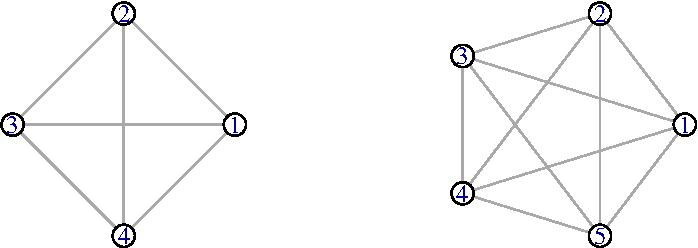
\includegraphics[width=\maxwidth]{figure/complete-graph-1} \caption[$K_4$ and $K_5$]{$K_4$ and $K_5$}\label{fig:complete-graph}
\end{figure}

\end{knitrout}

A *one-factor* $f_i$ is a set of edges in which each vertex
appears exactly once.

\begin{example}
Two possible one-factors of $K_4$ are:
$$f_1 = \{12,34\},\, f_2 = \{13,24\}$$
\end{example}

\begin{knitrout}
\definecolor{shadecolor}{rgb}{0.969, 0.969, 0.969}\color{fgcolor}\begin{kframe}
\begin{alltt}
\hlstd{targets}\hlopt{::}\hlkwd{tar_read}\hlstd{(}\hlstr{"two_one_factors_fig"}\hlstd{)}
\end{alltt}
\end{kframe}\begin{figure}
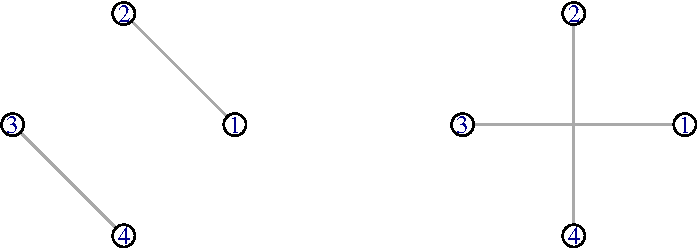
\includegraphics[width=\maxwidth]{figure/two-one-factors-1} \caption[Two one-factors of $K_{4}$]{Two one-factors of $K_{4}$}\label{fig:two-one-factors}
\end{figure}

\end{knitrout}

A *one-factorisation* of the complete graph is a set of
one-factors in which all possible edges (i.e. all unordered
pairs from the edge-set) appear exactly once.

\begin{knitrout}
\definecolor{shadecolor}{rgb}{0.969, 0.969, 0.969}\color{fgcolor}\begin{kframe}
\begin{alltt}
\hlstd{targets}\hlopt{::}\hlkwd{tar_read}\hlstd{(}\hlstr{"one_factorisation_fig"}\hlstd{)}
\end{alltt}
\end{kframe}\begin{figure}
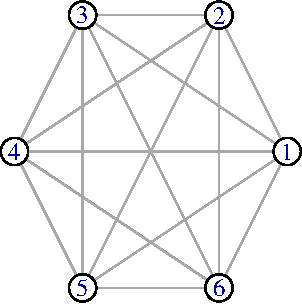
\includegraphics[width=\maxwidth]{figure/K6-1} \caption[$K_6$]{$K_6$}\label{fig:K6}
\end{figure}

\end{knitrout}

\begin{example}
Here
$G = K_6$
the complete graph on six vertices with
$$V = \{1, 2, 3, 4, 5, 6\}$$
$$E = \{12, 13, 14, 15, 16, 23, 24, 25, 26, 34, 35, 36, 45, 46, 56\}$$
The one-factors are

$$
f_1 = \{12, 35, 46\} \hspace{0.5cm}
f_2 = \{14, 23, 56\} \hspace{0.5cm}
f_3 = \{16, 25, 34\} \hspace{0.5cm}
f_4 = \{13, 26, 45\} \hspace{0.5cm} 
f_5 = \{15, 24, 36\}
$$
because
$f_1 \cup f_2 \cup f_3 \cup f_4 \cup f_5 = E$,
$F = \{f_1, f_2, f_3, f_4, f_5\}$
is a one-factorisation of
$G$,
shown in Figure~\ref{fig:one-factorisation}.
\end{example}

\begin{knitrout}
\definecolor{shadecolor}{rgb}{0.969, 0.969, 0.969}\color{fgcolor}\begin{kframe}
\begin{alltt}
\hlstd{targets}\hlopt{::}\hlkwd{tar_read}\hlstd{(}\hlstr{"orthogonal_one_factorisation_fig"}\hlstd{)}
\end{alltt}
\end{kframe}\begin{figure}
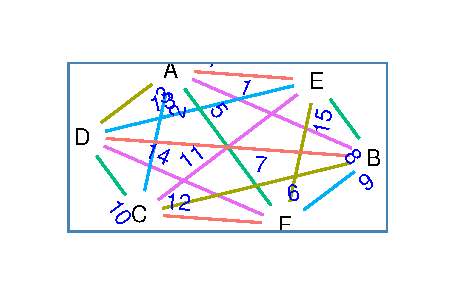
\includegraphics[width=\maxwidth]{figure/one-factorisation-1} \caption[One-factorisation of $K_6$]{One-factorisation of $K_6$}\label{fig:one-factorisation}
\end{figure}

\end{knitrout}

Two one factors $f$ and $l$ are said to be *orthogonal* if
$f \cap l$ contains at most one edge. Two one-factorisations
$F$ and $L$ are orthogonal if every one-factor in $F$ is
orthogonal to every one-factor in $L$.

Once again consider the square array in
\eqref{eq:roomsquare}.
If the individual elements within the array constituted the
vertex set of a graph (call it $R$) and the pairs within
each box of the array were edges, we know that each row is a
one-factor and each column is a one-factor (because each
member of $R$ occurs precisely once in each row and once in
each column). Further more, because all edges from the
edge-set of the complete graph (i.e. all unordered pairs
from $R$) appear once within the array, we know that the
rows together form a one-factorisation and the columns form
another, different, one-factorisation of $K_8$. Also,
because any row factor intersects any column factor in only
one pair (edge), all the row factors are orthogonal to all
the column factors and hence the two one-factorisations are
orthogonal. We have demonstrated the following theorem,
given in
\cite{dinitzContemporaryDesignTheory1992}
and proven in
\cite{nemethStudyRoomSquares1969}.

\begin{theorem}
The existence of a Room square of side $n$
is equivalent to the existence of two orthogonal
one-factorisations of the complete graph $K_{n+1}$.
\end{theorem}

An example is given in Figure 12 based on the Room square
in Table
\ref{tab:kirkman-curious}

XXX MISSING FIGURE XXX

\section{Hill-Climbing Algorithm for Room Squares}

The idea behind hill-climbing algorithms is to suppose
there exists a *neighbourhood* of feasible solutions to
some problem *instance*. With each *feasible* solution
there is an associated *cost* (or profit) and finding
an optimal solution becomes a matter of finding the solution
with minimum cost (or maximum profit).

A hill-climbing algorithm non-deterministically selects a
solution from the neighbourhood system such that the cost
is less than that of some initial solution until its
procedure fails, hence finding the locally optimal solution.

\subsection{An algorithm for one-factorisations}

Consider how to find a one-factorisation of the complete
graph. Here the problem instance is simply the even integer
$n$ and vertex set $V$.

Recall:

  - A one-factor of $K_n$ is a set of $n/2$ edges (hence
  $n$ is even) which partition $V$.

  - A one-factorisation of $K_n$ is a set of $n - 1$ one-factors
    which partitions the edge set of $K_n$.

Suppose we choose to represent a one-factorisation by a set
of $\frac{n}{2}(n - 1) = (n^2 - n)/2$ pairs each of the form
$(f_i, \{x, y\})$, where $x \neq y, i = 1 \ldots n - 1$,
and the following two conditions hold.

  1. Every $\{x, y\}$ occurs in a unique pair
  $(f_i, \{x, y\})$.

  2. For every one-factor $f_i$ and every vertex $x$,
  there is a unique pair of the form $(f_i, \{x, y\})$.

where $f_i$s are one-factors.

Then we consider a feasible solution to be a partial
one-factorisation, again represented by pairs having the
same form but this time,

  1. Every $\{x, y\}$ occurs in at most one pair
  $f_i, \{x, y\})$.

  2. For every one-factor $f_i$ and every vertex $x$ there
     is at most one pair of the form $(f_i, \{x, y\})$.

Where the $f_i$s are *partial one-factors*.

Which enables a definition for the cost of a feasible
solution $F$ to be given by:

$$c(F) = (n^2 - n)/2 - |F|$$

So that $F$ is a one-factorisation if and only if
$c(F) = 0$, i.e. $|F| = (n^2 - n)/2$

Now suppose that we can implement some procedure $X$, say,
which either reduces the cost or leaves it unaffected
(i.e. it never increases the cost) then the following
"hill-climbing" algorithm, provided it terminates,
will find a one-factorisation.

\begin{algorithm}[H]
  \While{$c(F) \neq 0$}{$X$}
\end{algorithm}

A procedure such as $X$ is called a heuristic.
The following two heuristics from
\cite{dinitzHillClimbingAlgorithmConstruction1987}
when used together are suitable for finding a
one-factorisation.

Let $F$ be a partial one-factorisation of $K_n$:

\begin{algorithm}[H]
\KwIn{any vertex $x$ such that $x$ does not occur in 
     every partial one-factor of $F$ (such a vertex is said
     to be a live point)}
\KwIn{any partial one-factor $f_i$ such that $x$ does
     not occur in $f_i$}
\KwIn{any $y \neq x$ such that there is no partial
     one-factor $f_j$ for which $(f_j,\{x,y\}) \in F$
     (we say that $x$ and $y$ do not occur together).}
\eIf{$y$ does not occur in $f_i$}{
  replace $F$ with $F \cup \{(f_i,\{x,y\})\}$
}{
  there is a pair in $F$ of the form $(f_i,\{z,y\}) (z \neq x)$.
  Replace $F$ with
    $F \cup \{(f_i,\{x,y\})\} \backslash \{(f_i,\{z,y\})\}$
}
\caption{$H_1$}
\end{algorithm}

\begin{algorithm}[H]
\KwIn{any partial one-factor $f_i$ which does not
     occur in exactly $n/2$ pairs in $F$ (such a partial
     one-factor is said to be live)}
\KwIn{any $x$ and $y$ such that $x$ and $y$ do not 
     occur together in $f_i$}
\eIf{$x$ and $y$ do not occur together}{
 Replace $F$ with $F \cup \{(f_i, \{x, y\})\}$
}{there is a pair in $F$ of the form $(f_j,\{x, y\}) (j \neq i)$.
  Replace $F$ with
    $F \cup \{(f_i,\{x,y\})\} \backslash \{(f_j,\{x,y\})\}$ }
\caption{$H_2$}
\end{algorithm}

Suppose we are in the process of trying to find a
one-factorisation for $K_6$, and have generated a partial
one-factorisation represented by the set $F$.

\begin{equation*}
F = \{(f_1,\{4,6\}),(f_1,\{3,5\}),(f_2,\{5,6\}),(f_3\{1,6\}), (f_3\{3,4\}),(f_4,\{2,3\}),(f_4,\{4,5\})\}
\end{equation*}

Now apply $H_1$.

  1. Choose $x = 2$. Live, because it doesn’t appear in
     $f_1, f_2, f_3$ or $f_5$.

  2. Of these four partial one factors, choose $f_1$.

  3. 2 only occurs together with 3 (in $f_4$),
     so pick $y = 5$.

  4. 5 already appears in $f_1$ so $\{z, y\} = \{3, 5\}$.
     So replace $F$ by
     $F \cup \{(f_1, \{2, 5\}) \backslash (f_1, \{3, 5\})\}$

So we have extracted one edge from the one-factorisation and
replaced it with another edge, leaving the cost unchanged.

If in 3. we had picked 1 then according to the heuristic we
should replace $F$ with $F \cup (f_1, \{2, 1\})$, increasing
$|F|$ by one, and so decreasing the cost by the same. Because
the cost cannot increase $H_1$ is a suitable heuristic for use
in a hill-climbing algorithm.

Now apply $H_2$ to the new one-factorisation
$F_1 = F \cup (f_1, \{2, 1\})$.

  1. We can pick any of $f_2, f_3, f_4, f_5$,
     because all are live. Choose $f_2$.

  2. Choose $x = 2, y = 3$,
     because neither appear in $f_2$.

  3. 2 and 3 occur together in $f_4$. So replace $F_1$
     with
     $F_1 \cup \{(f_2, \{2, 3\}) \backslash (f_4, \{2, 3\})\}$

Again the cost remains unchanged by this procedure,
and if in 2, we had chosen $x = 1, y = 4$ instead then
we would have replaced $F_1$ with
$F_1 \cup \{(f_2, \{1, 4\})\}$
decreasing the cost by one. As with $H_1$,
the cost cannot increase, which makes $H_2$ a suitable
heuristic.

The hill-climbing algorithm for constructing one-factorisations
which was first given in
\cite{dinitzHillClimbingAlgorithmConstruction1987}
has a very simple form.

\begin{algorithm}[H]
\While{$c(F) \neq 0$}{
  choose $r = 1$ or $r = 2$ with equal probability
  perform $H_r$}
\end{algorithm}

\subsection{An algorithm for Room squares}

To generate a Room square all that remains is to produce
another one-factorisation $G$, say, which is orthogonal to
$F$. This will inevitably require slight modifications to
be made to $H_1$ and $H_2$.

Now if an array $R$ is constructed in which the rows are
labelled with the one-factors of $F(f_1,f_2,...,f_{n-1})$,
and the columns are labelled with the partial one-factors
of $G(g_1,g_2,...,g_{n-1})$. Then $R$ will be a Room square
if the $(f_i,g_j)$ cell contains $\{x,y\}$, if and only if
$(f_i,\{x,y\}) \in F$ and $(g_j,\{x,y\}) \in G$ and is empty
otherwise.

Again these two heuristics are due to Dinitz and Stinson and
originally presented in
\cite{dinitzHillClimbingAlgorithmConstruction1987}.
Although a necessary correction has been made as will
become apparent.

\begin{algorithm}[H]
  1. Choose any live point $x$.

  2. Choose any partial one-factor $g_i$ such that $x$ does
     not occur in $g_i$.

  3. Choose any $y \neq x$ such that $x$ and $y$ do not occur
     together in $G$.

  4. Let $f_j$ be the one-factor of $F$ which contains the 
     edge $\{x, y\}$.
     
  \uIf{$R(f_j, g_i)$ is not empty}{
    $OH_1$ fails \;
  }
  \uElseIf{$y$ does not occur in $g_i$}{
    Replace $G$ by $G \cup (g_i, \{x, y\})$.

    Define $R(f_j, g_i)=\{x, y\}$.
  }
  \Else{
    there is a pair in $G$ of the form
     $(g_i, \{z, y\}) \hspace{0.5cm} z \neq x$.

    Replace $G$ by
    $G \cup (g_i, \{x, y\}) \backslash (g_i, \{z, y\})$.

    Define $R(f_k, g_i)$, to be empty$^i$,
    where $(f_k, \{z, y\}) \in F$.
  }
\caption{$OH_1$}
\end{algorithm}

\begin{algorithm}[H]
  1. Choose any live partial one-factor $g_i$.

  2. Choose any $x$ and $y \neq x$ such that $x$ and $y$
     do not occur together in $g_i$.

  3. Let $f_j$ be the one-factor of $F$ which contains
     the edge $\{x, y\}$.
  
  \uIf{$R(f_j, g_i)$ is not empty}{
    $OH_2$ fails
  }
  \uElseIf{$x$ and $y$ do not occur together}{
   Replace $G$ by $G \cup (g_i, \{x, y\})$.

   Define $R(f_j, g_i) = \{x, y\}$.
  }
  \Else{
    there is a pair in $G$ of the form
    $(g_k, \{x, y\}) \hspace{0.5cm} (k \neq i$)

       Replace $G$ by
       $G \cup (g_i, \{x, y\}) \backslash (g_k, \{x, y\})$

       Define $R(f_j, g_i) = \{x, y\}$.

       Define $R(f_j, g_k)$ to be empty.
  }
\caption{$OH_2$}
\end{algorithm}

\begin{example}
Suppose the factorisation $F$ from the earlier example has
been completed and is represented by the set:

\begin{equation}
  \begin{split}
    F = \{(f_1\{1,2\}),(f_1\{3,5\}),(f_1\{4,6\}),(f_2\{1,4\}),(f_2\{2,3\}),(f_2\{5,6\}), \\
    (f_3\{1,6\}),(f_3\{2,5\}),(f_3\{3,4\}),(f_4\{1,3\}),(f_4\{2,6\}),(f_4\{4,5\}),(f_5\{1,5\}),(f_5\{3,6\})\}
  \end{split}
\end{equation}

Notice that this is precisely the one-factorisation of $K_6$
given on page 9.

Now suppose we have established the following one-factors in
$G$:

\begin{equation}
  G = \{(g_1, \{1, 4\}), (g_2, \{1, 6\}), (g_3, \{3, 6\}), (g_5\{5, 6\}), (g_5\{1, 2\})\}
\end{equation}

At this state $R$ looks like 

\begin{equation}
  \begin{bmatrix}
     -  &   g_1    &    g_2    &    g_3   & g_4 &    g_5    \\
    f_1 &     -    &     -     &    -     &  -  & \{1, 2\}  \\
    f_2 & \{1, 4\} &     -     &    -     &  -  & \{5, 6\}  \\
    f_3 &     -    &  \{1, 6\} &    -     &  -  &     -     \\
    f_4 &     -    &     -     &    -     &  -  &     -     \\
    f_5 &     -    &     -     & \{3, 6\} &  -  &     -     \\
  \end{bmatrix}
\end{equation}

Now apply $OH_1$:

\begin{enumerate}
  \item{Choose $x = 5$, suitably live.}
  \item{Choose $g_3$, in which $5$ does not occur.}
  \item{$5$ does not occur together with $2$ in $G$, so we are
     free to choose $y = 2$.}
  \item{In $F$, $\{2, 5\} \in f_3$.}
  \item{
    $f_3, g_3$ is empty in $R$, also $y = 2 \notin g_3$.
    \begin{itemize}
       \item{Replace $G$ with $G \cup (g_3, \{5, 2\})$.}
       \item{Define $R(f_3, g_3) = \{5, 2\}$.}
    \end{itemize}
  }
\end{enumerate}

This decreases the cost by one, alternatively we might have
chosen, at stage 3. $y = 3$, in that case.

\begin{enumerate}
  \setcounter{enumi}{4}
  \item{$\{3, 5\} \in f_1$.}
  \item{
    $f_1, g_3$ is empty in $R$, also $y \in g_3$, occurring
      in the pair $(g_3, \{3, 6\}), z = 6$.
    \begin{itemize}
      \item{Replace $G$ with
        $G \cup (g_3, \{3, 5\}) \backslash (g_3, \{3,
        6\})$.}
      \item{Define $R(f_1, g_3) = \{3, 5\}$.}
      \item{Define $R(f_5, g_3)$ to be empty.}
    \end{itemize}
  }
\end{enumerate}

Which leaves the cost unaffected. Suppose now that $R$ is the
array after this second version of the application of $OH_1$:

\begin{equation}
  \begin{bmatrix}
     -  &   g_1    &    g_2    &    g_3   & g_4 &    g_5    \\
    f_1 &     -    &     -     & \{3, 5\} &  -  & \{1, 2\}  \\
    f_2 & \{1, 4\} &     -     &    -     &  -  & \{5, 6\}  \\
    f_3 &     -    &  \{1, 6\} &    -     &  -  &     -     \\
    f_4 &     -    &     -     &    -     &  -  &     -     \\
    f_5 &     -    &     -     &    -     &  -  &     -     \\
  \end{bmatrix}
\end{equation}

Now if we apply $OH_2$:

\begin{enumerate}
  \item{Choose $g_4$, a live partial one-factor.}
  \item{Choose $x = 1, y = 2$, neither of which occur in $g_4$.}
  \item{$(f_1, \{1, 2\}) \in F$.}
  \item{
    $f_1, g_4$ is empty in $R$, also $x$ and $y$ do occur
    together, $(g_5, \{1, 2\}) \in G$.
    \begin{itemize}
      \item{Replace $G$ with
       $G \cup (g_4, \{1, 2\}) \backslash (g_5, \{1, 2\})$}
      \item{Define $R(f_1, g_4) = \{1, 2\}$.}
      \item{Define $R(f_1, g_5)$ to be empty.}
    \end{itemize}
  }
\end{enumerate}

This procedure leaves the cost unaffected and if instead we had
chosen at $2$. $x = 3, y = 4$, then would have been required to
replace $G$ with $G \cup (g_4,\{3,4\})$, and put $\{3, 4\}$ in
cell $(f_3, g_4)$ of $R$, an action which reduces the cost by one.
However, we know that two orthogonal one-factorisations of $K_6$
are equivalent to a Room square of side 5, which has been shown
not to exist. Hence it would be futile to continue with this
method in this particular case. Nevertheless the example shows
how the heuristics work.
\end{example}

There is no guarantee of success with repeated use of these
heuristics, although Dinitz and Stinson are quick to point out that
the algorithm involving $H_1$ and $H_2$ has never
\footnote{In over ten-million attempts, they claim.}
failed to
produce the desired one-factorisation. If we hope to use the
$OH_1$ and $OH_2$ in a similar algorithm then the possibility of
failure becomes a real possibility.

Two possibilities exist, either both heuristics fail or
successive use of them leads to an infinite loop. In order to
avoid both we introduce a *threshold* function, which simply
arrests the progress of the algorithm after a certain number of
iterations of the heuristics. Dinitz and Stinson found after
experimentation that the following function is suitable.

\begin{equation}
T(n) = 100n
\end{equation}

Then the hill-climbing algorithm for finding a Room square is as
follows:

\begin{algorithm}[H]
\KwIn{Use the previous hill climbing algorithm to construct $F$,
     a one-factorisation of $K_n$.}
\KwIn{Number of iterations initialised to be $0$}
\While{(number of iterations $<T(n)$) and $c(G) \neq 0$}{
   Choose $r = 1$ or $r = 2$ at random with equal probability.
   Perform $OH_r$.
   Increment number of iterations.}
\end{algorithm}

\subsection{The Room Square Generator}

Dinitz and Stinson choose to implement the above algorithm in
Pascal, and ran in on an Amdahl 5850 workstation. It was very
successful, finding many Room squares with sides ranging from 11
to 101. For each successful trial they had 9 or 10 failures (the
program being stopped by the threshold function) and timings
ranged from 0.09 seconds for an 11x11 Room square, to 7.3 on
average for the 25 different 101x101 Room squares they found.

I chose to implement the hill-climbing algorithms in Visual Basic
6.0 on a Pentium III-450/Win 98 Desktop. Needless to say, it was
slightly less successful – exhibiting a similar probability of
success but unfortunately becoming very slow for Room squares
bigger than 21. It found square of side 21 after an all-night
search, but after 48 hours looking for one of 23x23 I decided to
call the search off.

Despite the failures at higher order, the Room square generator
was very successful in finding smaller squares. It found 7x7 Room
squares in as little as 4 seconds, and even 15x15 squares only
took a few minutes.

Annotated code for the Room square generator can be found along
with some of the larger squares in Appendix I and below is a
screen shot of the application having successfully located a 9x9
Room square in a little over one minute after 507 iterations of
the heuristics $OH_1$ and $OH_2$. The uppermost panel represents
some of the one-factorisation generated by the algorithm involving
$H_1$ and $H_2$, while the second panel shows part of the
orthogonal one-factorisation generated by $OH_1$ and $OH_2$. The
lower panel is a Room square of side 9.


\chapter{Proving the Existence of Room Squares}

\section{Introduction}

The theorem which will ultimately be established in section
4 relies upon a fundamental theorem in number theory – in
fact *the* fundamental theorem. The Fundamental Theorem of
Arithmetic states that every positive integer, except 1, can
be expressed uniquely as a product of primes. Proof of this
theorem can be found in
\cite{hardyIntroductionTheoryNumbers1979}.

The proof which established the existence of Room squares
will rely upon various other theorems which collectively
establish the existence of all Room squares with prime side,
except 3 and 5. Then multiplication theorems will be
developed to establish the existence of composite Room
squares (those whose side is the product of two or more
primes). Clearly if the prime Room squares can be proven to
exist, and hence composite Room squares, the fundamental
theorem will allow us to state that all Room squares exist
with odd positive integer side. Apart from a few exceptional
cases, this is basically what we wil be able to do.

\section{Starters, adders and cyclic Room squares}

\begin{equation}
  \begin{bmatrix}
    \infty 0 &     -    &     -    &     25     &     -    &     16     &    34    \\
      45     & \infty 1 &     -    &      -     &    36    &      -     &    20    \\
      31     &    56    & \infty 2 &      -     &     -    &     40     &     -    \\
       -     &    42    &    60    &  \infty 3  &     -    &      -     &    51    \\
      62     &     -    &    53    &     01     & \infty 4 &      -     &     -    \\
       -     &    03    &     -    &     64     &    12    &  \infty 5  &     -    \\
       -     &     -    &    14    &      -     &    05    &     23     & \infty 6 \\
  \end{bmatrix}
  \label{eq:cyclic}
\end{equation}

The Room square in \eqref{eq:cyclic} has a
special property. The pairs in any element of the array are
obtained by simply adding 1 (mod 7) to the pair in the
element immediately above and to the left; along with the
condition that

\begin{equation}
  \infty + 1 = \infty
\end{equation}

This special property means that the entire square can be
determined by the pairs in the first row, with successive
rows being developed in a cyclical manner according the
simple addition rule.  We call squares like \eqref{eq:cyclic} 
*cyclic* Room squares.

Also notice that $\{\infty,i\}$ occurs in position $(i,i)$.
A square with this property is said to be *standardised*. It
is important to realise that any Room square can be
standardised. As mentioned previously neither interchanging
the rows or columns nor permuting the symbol-set on which
the Room square is based has any effect of the
\`\`Room"-ness of that square.

The significance of cyclic Room squares is that the problem
of constructing a Room square is (potentially) reduced to
that of finding an appropriate first row. These rows cannot
be chosen arbitrarily, both the pairs used and the positions
in which they appear need to satisfy certain criteria, but
when they do exist a corresponding Room square always
exists. So proving the existence of this subclass of Room
squares is a matter only of proving the existence of these
special first rows.

\subsection{Finding a starter}

Suppose we wish to construct another Room square of the same
size as \eqref{eq:cyclic} based on the same
symbols. This new square will also be standardized so we
need only determine the three pairs that accompany
$\{0, \infty\}$ in the first row (the starter), and the
positions they occupy.

The set we will use to build our starter will be
${1, 2, \ldots, 6}$.

Each member of this set must occur exactly once in the pairs
of the starter – in order to satisfy the row condition for a
Room square.  Because of the cyclical construction the
condition is automatically true for successive rows if true
for the first.

Consider the existence in Table \ref{tab:cyclic-room} of an
arbitrary pair $\{a, b\}$. We know one of the following must be
true.

Either $\{2 + i, 5 + i\} = \{a, b\}$ or $\{1 + i, 6 + i\} = \{a, b\}$
or $\{3 + i, 4 + i\} = \{a, b\}$ for $i = 0, 1, 2, \ldots, 6$.
Say $a - b = 1$. Then $\{2 + i, 5 + i\} = \{a, b\}$ could never be
true because $(2 + i) - (5 + i) = -3\pmod 7 = 4$ and
$(5 + i) - (2 + i) = 3$. Similarly, the differences in $\{1, 6\}$
are $\pm 5$ so $\{a, b\}$ couldn’t be generated from $\{1, 6\}$.

However, $(4 + i) - (3 + i) = 1$ so $\{a, b\}$ will inevitably be
generated by $\{3, 4\}$ for some value of $i = 0, 1, \ldots, 6$.
e.g. $\{2, 3\} = \{3 + 6, 4 + 6\}$

Because $a$ and $b$ separately take on all values from
$\{0, 1, 2, \ldots, 6\}$, their differences will similarly take on
all these values (except 0 because there are no pairs of the form
$\{a, a\}$) and so an essential property for the starter must be
that the six differences generated by its three pairs contain all of
$\{1, 2, \ldots, 6\}$.

When a starter satisfies this property, and the condition
that the pairs contain in their union all of
$\{1, 2, \ldots, 6\}$, it is clear that it will inevitably generate
the correct pairs which populate a 7x7 Room square.  There
are three pairs in the starter, each generates seven unique
pairs under cyclical construction, which along with the
seven pairs generated by $\{0, \infty\}$ counts for all the
28 unordered pairs from $\{\infty, 0, 1, \ldots, 6\}$.

A starter for larger Room squares of course has to obey the same
criterion. We include a general definition based on
\cite{dinitzContemporaryDesignTheory1992}.

If $G$ is an additive Abelian group of order $g$, then a
*starter* in $G$ is a set of unordered pairs:
$$S = \{\{s_i, t_i\}:1 \leq i \leq (g - 1)/2\}$$
which satisfies these properties:

\begin{enumerate}
  \item{$\{s_i:1 \leq i \leq (g-1)/2\} \cup \{t_i : 1 \leq i \leq (g-1)/2\} = G \backslash \{0\}$}
  \item{$\{\pm (s_i - t_i ) : 1 \leq i \leq (g-1)/2 \} = G \backslash \{0\}$}
\end{enumerate}

Whenever we have any $t$ sets $D_1, \ldots, D_t$ each of
size $k$ in which each non-zero member of an additive
abelian group can be represented as a difference between
members of the $D_i \lambda$ times, we say those sets form a
*difference system*.

Much use will be made of difference systems throughout this
work. Notice that the definition of a starter presumes
standardization, and therefore that $\{\infty, i\}$ is in
position $(i, i)$. The following pairs form a starter in
$G = \{0, 1, 2, \ldots, 6\}$ (an additive abelian group with
order $g = 7$.)

\begin{equation}
\{1,3\} \{2,6\} \{4,5\}
\end{equation}

Property 1 is satisfied because
$\{1,3\} \cup \{2,6\} \cup \{4,5\} = G \backslash \{0\}$

Property 2 is also satisfied because

\begin{equation}
\begin{split}
\{1 - 3 = 5, 3 - 1 = 2, 2 - 6 = 3, 6 - 2 = 4, 4 - 5 = 6, 5 - 4 = 1\} &= \{1, 2, 3, 4, 5, 6\} \\
 &= G\backslash \{0\}
\end{split}
\end{equation}

Hence

\begin{equation}
  \begin{bmatrix}
    \infty 0 &  13 &  26 &  45 \\
    \infty 1 &  24 &  30 &  56 \\
    \infty 2 &  35 &  41 &  60 \\
    \infty 3 &  46 &  52 &  01 \\
    \infty 4 &  50 &  63 &  12 \\
    \infty 5 &  61 &  04 &  23 \\
    \infty 6 &  02 &  15 &  34
  \end{bmatrix}
  \label{eq:starter}
\end{equation}

are all the unordered pairs from $\{\infty, 0, 1, \ldots, 6\}$
sorted into seven rows that contain each of
$\{\infty, 0, 1, \ldots, 6\}$ exactly once. All that remains is to
determine the columns.

\subsection{Finding an adder}

In constructing the starter we made use of the fact that
each row has to contain each symbol exactly once and all
unordered pairs from the symbol set have to occur exactly
once in the whole array. The remaining condition – namely,
that each symbol must occur once in each column – is now
employed to finish the construction.

Again, because of the cyclical nature of Room squares
generated from starters we can be sure that if one column
contains each member of the symbol set, all columns will.

Also, because we have decided to construct a standardized
Room Square we know that column $i$ contains $\{\infty,i\}$.
So the final column (column 6) contains $\{\infty,6\}$, and
depending on where we place the starter pairs it will also
include: $$\{1,3\}+x \hspace{1cm} \{2,6\}+y \hspace{1cm}
\{4,5\}+z$$ For some distinct values of $x,y$ and $z$ (only
one pair allowed per box).\ Considering that the new pairs
to form column 6 must contain in their union each of
$\{0,1,2,...,5\}$ we build the following table.

\begin{equation}
  \begin{bmatrix}
    x &  13 + x & 26 + y & z & 45 + z \\
    0 &    13   &   26   & 0 &   45   \\
    1 &    24   &   30   & 1 &   56   \\
    2 &    35   &   41   & 2 &   60   \\
    3 &    46   &   52   & 3 &   01   \\
    4 &    50   &   63   & 4 &   12   \\
    5 &    61   &   04   & 5 &   23   \\
  \end{bmatrix}
  \label{eq:adder}
\end{equation}

Our task is simply to determine three unique values for $x,
y$ and $z$ such that $13 + x, 26 + y$ and $45 + z$ contain
in their union each of $\{0, 1, 2, \ldots, 5\}$. These
values will then determine the positions to place 13, 26 and
45 in row 1.

Choosing 4 from the first column corresponds to having 50
appear in the final column of the Room Square and forces the
selection of $y = 2$ from the next column of the table, (41
being the only pair not containing any of the already used
5, 6 or 0). 23 is the only possible choice from the final
column, accompanied by a value of $z = 5$. These three
numbers are known as an *adder* corresponding to the starter
13, 26, 45. This is not necessarily the only adder.

If 50 is to be generated in the final column of the Room
square by the pair 13 in the first row, then 13 must go in
column $7 - 4 = 3$. Similarly 26 has to be put in column
$7 - 2 = 5$ and 45 in $7 - 5 = 2$.  We can now construct our
cyclic room square.

\begin{equation}
  \begin{bmatrix}
    \infty 0 &  45 &  13 &   - &  26 &   - &   - \\
     - &  \infty 1 &  56 &  24 &   - &  30 &   - \\
     - &   - &  \infty 2 &  60 &  35 &   - &  41 \\
    52 &   - &   - &  \infty 3 &  01 &  46 &   - \\
     - &  63 &   - &   - &  \infty 4 &  12 &  50 \\
    61 &   - &  04 &   - &   - &  \infty 5 &  23 \\
    34 &  02 &   - &  15 &   - &   - &  \infty 6 
  \end{bmatrix}
  \label{eq:cyclic-room}
\end{equation}

In general, we define an adder by considering the elements
which must accompany $\{\infty, 0\}$ in column 0. Therefore
an adder is defined in the following way:

An *adder* for a starter
$S = \{\{s_i, t_i\}: 1 \leq i \leq (g - 1)/2 \}$
is a set of $(g - 1)/2$ distinct non-zero elements
$a_1, a_2, ..., a_{(g - 1)/2}$ of $G$ such that:
$s_1 + a_1, t_1 + a_1, s_2 + a_2, \ldots, s_{(g - 1)/2} + a_{(g - 1)/2}, t_{(g - 1)/2} + a_{(g - 1)/2}$
are precisely all the non-zero elements of $G$.

The *starter-adder* method employed in the above example was
introduced
\footnote{Both Howell and Whitfield had previously found starters and adders, but the precise method used here due to Stanton and Mullin.}
by
\cite{stantonConstructionRoomSquares1968},
who used it to construct Room squares of side 11.
They also went on to apply the method to larger squares and
gave the first real suggestions that the number of Room squares
is infinite.

Two simple lemmas given in
\cite{stantonConstructionRoomSquares1968}
demonstrated that the problem of finding starters for larger
Room squares was straightforward. In fact they can be
guaranteed always to exist, and the only difficulty comes
from finding a corresponding adder, which is not guaranteed
to exist.

\begin{lemma}
In an additive abelian group $G$ of order $g = 2n-1$,
then pairs
\begin{equation*}
  \{n - 1, n\}, \{n - 2, n + 1\}, \{n - 3, n + 2\}, \{n - 4, n + 3\}, \ldots\{1, 2n - 2\}
\end{equation*}
are a starter for a Room square of side $2n - 1$.
\end{lemma}

\begin{example}
A Room square of side $2n - 1 = 19$.

\begin{equation*}
S_{19} = \{\{9, 10\}, \{8, 11\}, \{7, 12\}, \{6, 13\}, \{5, 14\}, \{4, 15\}, \{3, 16\}, \{2, 17\}, \{1, 18\}\}
\end{equation*}
is a starter.

Indeed, the differences are
\begin{equation*}
\begin{split}
  & \{\pm(10 - 9), \pm(11 - 8), \pm(12 - 7), \pm(13 - 6), \pm(14 - 5), \pm(3 - 16), \pm(2 - 17), \pm(18 - 1)\} \\ 
  &= \{1, 18, 3, 16, 5, 14, 7, 12, 9, 10, 8, 11, 6, 13, 4, 15, 2, 17\} \\
  &= G \backslash \{0\}
\end{split}
\end{equation*}
\end{example}

\begin{lemma}
In the Galois field of order $k - 1$, with primitive root
$a$ the following pairs form a starter for a Room square of
side $k$.
\begin{equation}
  \{a, a^n\}, \{a^2, a^{n + 1}\}, \{a^3, a^{n + 2}\}, \ldots, \{a^{n - 1}, a^{2n - 2}\}
\end{equation}
\end{lemma}

\begin{example}
A Room square of side $2n - 1 = 23$. $n = 12$. $a = 5$.
The set of pairs
\begin{equation*}
\begin{split}
S_{23} &= \{\{5, 5^{12}\}, \{5^2, 5^{13}\}, \{5^3, 5^{14}\}, \ldots, \{5^{11}, 5^{22}\}\} \\
       &= \{\{5, 18\}, \{2, 21\}, \{10, 13\}, \{4, 19\}, \{20, 3\}, \{8, 15\}, \{17, 6\}, \{16, 7\}, \{11, 12\}, \{9, 14\}, \{22, 1\}\}
\end{split}
\end{equation*}
is a starter.
\end{example}

On closer inspection the two types of starters are
identical
\footnote{The starter in then first Lemma has pairs whose elements always
    sum to $2n-1$, while the second Lemma, because $a^{n-1}=-1$, has
    pairs which can be written in the form $(a^x,-a^x)$.},
with a general element being of the form
$$\{j,-j\}$$

Starters of this form are called *patterned* starters.

Stanton and Mullin went on to show that using the method
outlined in Example 2.1 they could find adders corresponding
to the patterned starters for $k = 7, 11, 13, 15, 17$. They had
problems with 9 (but were able to construct one using a
different method) and finding it too laborious for $k > 19$
they developed an algorithm which, when implemented in
Fortran, was able to find patterned starters with adders for
all odd $k$ up to 49, with no further gaps. Suggesting the
possibility (which they conjectured) that there are Room
squares for all odd side greater than 5.

They also found an interesting result regarding the number
of Room Squares which could be obtained from patterned
starters, summarised in table \ref{tab:patterned}. 

\begin{table}[h!]
  \begin{center}
    \caption{Number of patterned Room squares (PRS)}
    \label{tab:patterned}
    \begin{tabular}{c|c}
    Value of $k$ & Number of PRS \\ \hline
    7 & 2 \\
    9 & 0 \\
    11 & 4 \\
    13 & 8 \\
    15 & 44 \\
    17 & 416 \\
    19 & The program was turned off after the production of 967 PRS
    \end{tabular}
  \end{center}
\end{table}

Stanton and Mullin’s results suggest that the number of PRS
(patterned Room squares) increases very rapidly. Which,
bearing in mind that the PRS are a sub-class of CRS (cyclic
Room squares), which are in turn a sub-class of Room
squares, implies that there are vast numbers of Room squares
of large order.

Before introducing a class of starters for which the
existence of a corresponding adder is guaranteed we quickly
confirm that when a starter and adder exist then a Room
square will always result. This seems obvious from the
method outlined in the previous section, but now we prove it
explicitly.

\begin{theorem}
\label{thm:starter-adder}
If an Abelian group $G$ of odd order $2n - 1$ admits a starter
and an adder, then there exists a Room square of order $2n$.
\end{theorem}

\begin{proof}
A square is constructed on the set $G \cup \{\infty\}$, where $G$ is an
additive Abelian group of order $2n-1$.

\begin{equation}
G = \{g_0 = 0, g_1, g_2, \ldots, g_{2n-2}\}
\end{equation}

The columns and rows of the square are labelled as follows:

\begin{equation}
  \begin{bmatrix}
        -      & g_0  &  g_1  &  g_2  & \ldots &  g_{2n - 1} \\
       g_0     &   -  &   -   &   -   &    -   &     -       \\
       g_1     &   -  &   -   &   -   &    -   &     -       \\
       g_2     &   -  &   -   &   -   &    -   &     -       \\
     \vdots    &   -  &   -   &   -   &    -   &     -       \\
    g_{2n - 1} &   -  &   -   &   -   &    -   &     -       \\
  \end{bmatrix}
\end{equation}

If a starter
$\{\{s_1, t_1\}, \{s_2, t_2\} \ldots \{s_{n - 1}, t_{n - 1}\}\}$
and an
adder $\{a_1, a_2, \ldots, a_{n - 1}\}$ can be obtained from
$G$ and if the square is populated by pairs of elements from
$G$ according to the following rules:

\begin{enumerate}
  \item{$\{\infty, g_i\}$ goes in $(g_i, g_i)$}
  \item{While $\{s_i + g_i, t_i + g_i\}$ goes in $(g_i, g_i - a_i)$}
\end{enumerate}

for all $g_i \in G$. The resulting square will be a Room square on
$G \cup \{\infty\}$.

\begin{enumerate}
  \item{Row $g_0 = 0$, contains the pairs
      $\{s_i, t_i\}:1 \leq i \leq n-1$,
      which are the elements of the starter,
      hence all of $G \backslash \{0\}$. These pairs are
      accompanied by $\{\infty, 0\}$, so row 0 contains all
      of $G \cup \{\infty\}$. Subsequent rows simple
      contain a permutation of the same elements, hence
      the \emph{row property} of Room squares is satisfied for
      all rows.}
  \item{As mentioned before, the starter forms a difference
      system in $G \backslash \{0\}$, so all unordered
      pairs of this set occur along with all unordered
      pairs of the form
      $\{\infty, g_i\}: 1 \leq i \leq n - 1$,
      hence \emph{all unordered pairs from}
      $G \cup \{\infty\}$ \emph{occur} in the square exactly once.}
  \item{All pairs of the form $\{s_i + a_i, t_i + a_i\}$ go in
      $(a_i, 0)$, i.e. column 0. According to the
      definition of a starter these pairs are all of $G
      \backslash \{0\}$, and we know that $\{\infty,0\}$
      is also in column 0. So the first column, and hence
      all others, contains all of $G \cup \{\infty\}$,
      thus satisfying the \emph{column property} of Room
      squares.}
\end{enumerate}
\end{proof}

\section{Strong Starters}

The next state in proving the existence of Room squares came
about, not by continuing to try to find adders for starters
that were already known (the patterned starters, for
example), but when
\cite{mullinFurnishingRoomSquares1969},
discovered a
class of starters that generated their own adders.

\begin{theorem}
\label{thm:furnishing}
Suppose a starter
$\{\{s_1, t_1\}, \{s_2, t_2\}, \ldots, \{s_{(g - 1)/2}, t_{(g - 1)/2}\}\}$
exists, such that the sums of each pair
$(s_1 + t_1, s_2 + t_2, etc...)$
are all distinct and non-zero, then that starter is said
to be strong, and
\begin{equation}
 A(S) = \{a_i = -(s_i + t_i):1 \leq i \leq (g - 1)/2\}
\end{equation}
is an adder for a starter.
\end{theorem}

\begin{proof}
\begin{enumerate}
  \item{The $a_i$ are all distinct and non-zero
    All the $(s_i + t_i)$ are, by definition, distinct
    and non-zero. Therefore all the $a_i = -(s_i + t_i)$ are
    distinct and non-zero.}
  \item{$s_1 + a_1, t_1 + a_1, s_2 + a_2, \ldots, s_{(g - 1)/2}, t_{(g - 1)/2} + a_{(g - 1)/2}$
    are precisely all the non-zero elements of $G$.
    \begin{align*}
      s_1 + a_1 = s_1 - (s_1 + t_1) = -t_1 &= t_{(g - 1)/2}  \\
      t_1 + a_1 = t_1 - (s_1 + t_1) = -s_1 &= s_{(g - 1)/2}  \\
      s_{(g - 1)/2} + a_{(g - 1)/2} = -t_{(g - 1)/2} &= t_1  \\
      t_{(g - 1)/2} + a_{(g - 1)/2} = -s_{(g - 1)/2} &= s_1 
    \end{align*} }
      Are all the non-zero elements of $G$ in reverse order.
\end{enumerate}
(Notice that the patterned starter is not strong, on the
contrary, the sums of its pairs are all identical.)
\end{proof}

\begin{example}
The pairs $(5, 7)(11, 6)(2, 8)(9, 12)(10, 1)(3, 4)$,
constitute a strong starter for a Room square of side 13,
based on $G = Z_{13}$.

Firstly, the pairs satisfy the conditions for being a
starter, as the union of all pairs is equal to
$G \backslash \{0\}$, and similarly the differences are all of
$G\backslash \{0\}$.
Secondly the sums of the pairs,
respectively $12, 4, 10, 8, 11, 7$ are all distinct and
non-zero.
Therefore an adder is
$\{-12, -4, -10, -8, -11, -7\} = \{1, 9, 3, 5, 2, 6\}$
So the following is a legitimate first row for a cyclic
Room square of order 14.

\begin{equation}
  \begin{bmatrix}
    \infty, 0 & - & - & - & 11,6 & - & - & 3,4 & 9,12 & - & 2,8 & 1,10 & 5,7 \\
  \end{bmatrix}
\end{equation}

\end{example}

Mullin and Nemeth originally discovered strong starters for
Room squares embedded within another type of combinatorial
design, known as a Steiner triple system. With these they
were able to prove that Room squares exist for all sides
$v = 1\pmod 6$. Rather than examine this approach we move on to
a type of starter which provides its own adder.

\section{Mullin-Nemeth Starters}

If $x$ is a primitive element in $G = GF(p^n)$, then the elements
$x^1, x^2, \ldots, x^{p^n - 1} = 1$ are, by definition, all of
$G \backslash \{0\}$. Alternatively, we can write
$G \backslash \{0\} = \{x^0 = 1, x^1, \ldots, x^{p^n - 2}\}$.

\begin{example}
The field $GF(23)$ has a primitive root $x = 5$, because
$5^0 = 1$, $5^1 = 5$, $5^2 = 2$, $5^3 = 10$, $5^4 = 4$,
$5^5 = 20$, $5^6 = 8$, $5^7 = 17$, $5^8 = 16$, $5^9 = 11$,
$5^{10} = 9$ $5^{11} = 22$, $5^{12} = 18$, $5^{13} = 21$,
$5^{14}  =13$, $5^{15} = 19$, $5^{16} = 3$, $5^{17} = 15$,
$5^{18} = 6$, $5^{19} = 7$, $5^{20} = 12$, $5^{21} = 14$
are all the non-zero elements of $GF(23)$.
\end{example}

\cite{mullinFurnishingRoomSquares1969}
used the theory
of primitive elements to create strong starters in the
additive group of (nearly) any Galois field of prime-power
order. Which, because theorems
\ref{thm:starter-adder}
and
\ref{thm:furnishing}
were already
known, was equivalent to proving the existence of Room
squares for (nearly) all orders $p^n + 1$. Before
introducing the general construction for these starters, we
illustrate the basic method with a couple of examples of
particular cases.

\begin{example}
\label{ex:strong-starter}
We can create a strong starter from Example 2.5 simply by
pairing the elements in the order in which they were
generated.
\begin{equation}
S = \{\{1, 5\}, \{2, 10\}, \{4, 20\}, \{8, 17\}, \{16, 11\}, \{9, 22\}, \{18, 21\}, \{13, 19\}, \{3, 15\}, \{6, 7\}, \{12, 14\}\}
\end{equation}
is a strong starter.

Obviously each member of $GF(23)$ occurs once, because of
the definition of a primitive root.  The differences
\begin{equation}
  \{\pm 4, \pm 8, \pm 7, \pm 9, \pm 10, \pm 5, \pm 3, \pm 6, \pm 11, \pm 1, \pm 2\}
\end{equation}
are similarly all of $GF(23)$, so $S$ is a
starter. The sums
\begin{equation}
  \{6, 12, 1, 2, 4, 8, 16, 9, 18, 13, 3\}
\end{equation}
are all
unique, and therefore $S$ is strong and
\begin{equation}
  A = \{17, 11, 22, 21, 19, 15, 7, 14, 5, 10, 20\}
\end{equation}
is an adder for $S$. So, the following row will generate a
Room square of order 24 under cyclic construction.

\begin{equation}
  \begin{bmatrix}
    \infty, 0 & 4,20 & 8,17 & 12,14 & 16,11 & - & 1,5 & - & 9,22 & 13,19 & - & - & 2,10 & 6,7 & - & - & 18,21 & - & 3,15 & - & - & - & - \\
  \end{bmatrix}
\end{equation}

\end{example}

This is an example of the simplest case of the general
theorem of Mullith and Nemeth, where the Galois field is $Z_p$
(the integers mod $p$), with $p = 23 = 3\pmod 4$ a prime.

\begin{theorem}
\label{thm:strong-starter}
If $p = 4m + 3$ is prime, $m \geq 1$, then
\begin{equation}
S = \{\{x^0, x^1\}, \{x^2, x^3\}, \ldots, \{x^{4m}, x^{4m+1}\}\}
\end{equation}
is a strong starter in $Z_p$, and hence a Room square of
order $p + 1$ exists.
\end{theorem}

Example
\ref{ex:strong-starter}
took $m = 5$ and $x = 5$.

A slightly more general version of Theorem
\ref{thm:strong-starter},
which we
prove instead, involves any field of prime power order where
$p^n = 2t + 1$, with $t > 1$ and odd. Of course, when $p^n$ is not
prime, the field will no longer be the integers modulo $p$,
instead the primitive element will be an irreducible
polynomial whose coefficients belong to $Z_p$.

\begin{theorem}
\label{thm:strong-starter-2}
If $p^n = 2t + 1 = 3\pmod 4$ then
\begin{equation*}
S = \{\{x^0, x^1\}, \{x^2, x^3\}, \ldots, \{x^{2t - 2}, x^{2t - 1}\}\}
\end{equation*}
is a strong starter in $GF(p^n), (p^n \neq 3)$
\end{theorem}

\begin{proof}
$x$ is a primitive element, so the elements in the starter
are all the non-zero members of $GF(P^n)$.  The differences
are, respectively
\begin{equation*}
\pm x^0(1 - x), \pm x^2 (1 - x), \ldots, \pm x^{2t - 2}(1 - x)
\end{equation*}
$(1 - x)$ is a non-zero ($x = 1$ is not primitive) member of
$GF(p^n)$.

So in order to show that these differences are all the $2t$
non-zero members of $GF(p^n)$ we merely need to prove that
the $2t$ differences are all distinct and non-zero.

All the differences can be written
$\pm x^{2i}(1 - x)$, $0 \leq i \leq t - 1$

$(1 - x) \neq 0$

$x^{2i}(1 - x) = x^{2j}(1 - x)$

$\Rightarrow x^{2i} = x^{2j}$
$\Rightarrow i = j$,
because $0 \leq 2i, 2j \leq 2t - 2 < p^{n - 1}$,
and the primitive element, by definition,
produces each element of $GF(p^n)$ exactly once as the
indices range from 0 to $p^{n - 1}$.  Similarly
$-x^{2i}(1 - x) = -x^{2j}(1 - x)$ only when $i = j$.
So all the positive differences are unique, similarly the negative.
However, there remains a possibility for repetition when the
signs are opposite:

\begin{equation}
\label{eq:signs}
x^{2i}(1 - x) = -x^{2j}(1 - x)
\end{equation}

Either $i = j$ or $i \neq j$.

Let $i = j$,

\eqref{eq:signs} becomes
$x^{2i} + x^{2i} = 0, \Rightarrow 2x^{2i} = 0$,
but $i$ takes values $0 \ldots t - 1$, so $x^2 = 0$ when $i = 1$,
contradicting the order of the primitive element.  In the
$i \neq j$ case, we assume (without loss of generality) that
$i < j$ and write $x^{2i} = -x^{2j}$. As
$x^{2i}(1 + x^{2j - 2i}) = 0$ it follows that $x^{2j - 2i} = -1$

In $GF(2t + 1)$, $x^{\frac{1}{2}(q - 1)} = x^t = -1$

\begin{equation*}
2j - 2i = t
\end{equation*}

but this is a contradiction as we insisted that $t$ be odd.

So $S$ is a starter.

To prove that $S$ is strong we simply note that the sums can
be written:

\begin{equation*}
x^0(1 + x), x^2(1 + x), \ldots, x^{2t - 2}(1 + x)
\end{equation*}

$1 + x = 0 \Rightarrow x = -1$ is only true when $p^n = 3$.

So $(1 + x) \neq 0$.

So $x^{2i}(1 + x) = x^{2j}(1 + x) \Rightarrow x^{2i} = x^{2j}$.

We have already shown that $x^{2i} = x^{2j}$ is only true for
$i = j$.

So all the sums are unique, and the starter is strong.

Hence, by Theorems
\ref{XXX}
and
\ref{XXX},
Room squares exist for all
$p^n\equiv 3\pmod 4$, and in the case when
$p^n\equiv 3\pmod 4$ is
prime, these Room squares are based on $Z_p$.
\end{proof}

The most generalised case of Mullin and Nemeth’s theorem
proves the existence of Room squares for all prime powers
$p^n = 2^kt + 1$ where $k > 1$ and $t > 1$ is odd ($k$ and $t$,
both positive integers), and reduces to Theorem
\ref{thm:strong-starter}
when $k = 1$.

\begin{theorem}
\label{thm:strong-starter-3}
A strong starter exists in $GF(p^n)$, where $p^n = 2^kt + 1$
(with $k > 1$ and $t > 1$ is odd).
\end{theorem}

\begin{proof}
Let $d = 2^{k-1}$.

Then the strong starter in question looks like this:

\begin{equation*}
S = \left\{
  \begin{array}{cccc}
    (x^0,x^d) & (x^{2d},x^{3d}) & \ldots & (x^{(2t - 2)d},x^{(2t - 1)d}) \\
    (x^1,x^{d + 1}) & (x^{2d + 1},x^{3d + 1}) & \ldots & (x^{(2t - 2){d + 1}},x^{(2t - 1){d + 1}}) \\
    \vdots & \vdots & \ldots & \vdots \\
    (x^{d - 1},x^{2d - 1}) & (x^{3d - 1},x^{4d - 1}) & \ldots & (x^{(2t - 2){d - 1}},x^{2td - 1})
  \end{array}
\right\}
\end{equation*}

Where the pairs have been placed in an array to emphasise
that, when read vertically, this is an exhaustive list of
all the non-zero elements of $GH(p^n)$, ordered according to
powers. Of course, in the $k = 1, d = 1$ case this starter
reduces to the one quoted in Theorem
\ref{thm:strong-starter-2}.

To prove that $S$ is a starter we need also to show, as
usual, that the differences between pairs are all of
$GF(p^n)$, and to show that the starter is strong we need to
show that the sums of pairs are all distinct and non-zero.

The differences can be written in the following scheme:

\begin{equation*}
  \begin{array}{cccc}
    x^0(1 - x^d), & x^{2d}(1 - x^d), & \ldots, & x^{(2t - 2)d}(1 - x^d) \\
    x^1(1 - x^d), & x^{2d + 1}(1 - x^d), & \ldots, & x^{(2t - 2)d + 1}(1 - x^d) \\
    \vdots & \vdots & \ldots & \vdots \\
    x^{d - 1}(1 - x^d), & x^{3d - 1}(1 - x^d), & \ldots, & x^{(2t - 1)d - 1}(1 - x^d)
  \end{array}
\end{equation*}

The order of $x$ is $p^n-1 = 2^kt = 2^{k-1}2t = 2td > d$,
(meaning $x^{2td} = 1$ and $x^\alpha \neq 1$ when
$1 \leq \alpha < 2dt$) and so $x^d \neq 1$, so $(1 - x^d) \neq 0$.
We can write the differences in a general form:

\begin{equation}
\pm x^{2id + j}(1 - x^d), 0 \leq i \leq t-1, 0 \leq j \leq d-1
\end{equation}

If there were repetition, either of the
form $D = D$ or $-D = -D$, where $D = x^{2id + j}(1 - x^d)$,
then the following must hold:

\begin{equation}
\pm x^{2id + j}(1 - x^d) = \pm x^{2Id + J}(1 - x^d)
\end{equation}

Cancelling by $(1 - x^d)$, legitimate because $(1 - x^d) \neq 0$,
gives:

\begin{equation}
x^{2id + j} = -x^{2ID + J}
\end{equation}

dividing through by $x^{2Id + j}$ leaves

\begin{align*}
  x^{2id - 2Id} &= x^{J = j} \\
  x^{2d(i - I)} &= x^{J - j}
\end{align*}

But if $i \neq I$, then the LHS has an index which is an
integer multiple of $d$. The index in the RHS, however, can
never be an integer multiple of $d$ because $J$ and $j$
range over the integers $0 \ldots d - 1$.  So the only possibility
for equality is when both indices are zero, i.e. $i = I$ and
$j = J$.

As in the previous proof we have to deal with the
possibility of repetition for differences of opposite sign.

For coincidence we require:

\begin{align*}
  x^{2id + j} &= -x^{2ID + J} \\
  x^{2id + j} + x^{2Id + J} &= 0
\end{align*}

We assume that $2id + j < 2Id + J$ and rewrite this expression
as:

\begin{equation}
x^{2id + j}(1 + x^{(2I - 2i)d + (J - j)}) = 0
\end{equation}

Which implies that $x^{(2I - 2i)d + (J - j)} = -1$.

But in $GF(q)$, $x^{\frac{1}{2}(q - 1)} = -1$. Where, in this
case $q - 1 = 2^kt$, so $\frac{1}{2}(q - 1) = 2^{k - 1}t = dt$.

Therefore, $x^{dt} = -1$ and so $(2I - 2i)d + (J - j) = dt$.

Thus, $(J - j)$ is an integer multiple of $d$ or zero.

But $J$ and $j$ both take only the values $0 \ldots d-1$, so
$(J - j)$ is in the interval $[1 - d, d - 1]$ and hence must
be zero, leaving

\begin{eqnarray*}
  (2I - 2i)d &= dt \\
  2I - 2i &= t
\end{eqnarray*}

But $t$ is strictly odd, and so we have reached a
contradiction, hence the differences are all unique, belong
to $GF(p^n)$ and there are $2td$ of them, hence each member
of $GF(p^n)$ occurs exactly once as a difference. So $S$ is
a starter. To prove that the starter is strong we write the
sums as

\begin{equation*}
  \begin{array}{cccc}
    x^0(1 + x^d), & x^{2d}(1 + x^d), & \ldots, & x^{(2t - 2)d}(1 + x^d) \\
    x^1(1 + x^d), & x^{2d + 1}(1 + x^d), & \ldots, & x^{(2t - 2)d + 1}(1 + x^d) \\
    \vdots & \vdots & \ldots & \vdots \\
    x^{d - 1}(1 + x^d), & x^{3d - 1}(1 + x^d), & \ldots, & x^{(2t - 1)d - 1}(1 + x^d)
  \end{array}
\end{equation*}

and notice that $x^d = -1 \Rightarrow d = dt$ (because
$x^{dt} = -1) \Rightarrow t = 1$, but instead we insisted that
$t$ be strictly greater than one (this being the reason
why). So $(1 + x^d) \neq 0$ and the above argument
involving $(1 - x^d)$ can be invoked, replacing
$(1 - x^d)$ by $(1 + x^d)$.

So $S$ is a strong starter, and the general theorem of
Mullin and Nemeth is proven, guaranteeing the existence of a
vast class of Room Squares.
\end{proof}

\section{The Trouble with Fermat Numbers}

Unfortunately, in establishing the Mullin-Nemeth starters
we were forced to exclude a similarly vast, potentially
infinite, class of Room squares by insisting that $t$ be
strictly greater than one. These exceptional Room squares
have side $2^k + 1$.

Rectifying this problem is essential if we are to prove the
existence of Room squares. As mentioned previously, the
proof relies on a multiplication theorem, so proving that
all the prime Room squares exist is vital. Although the
theorem of Mullin-Nemeth will take care of all squares
with prime power side, the multiplication theorem is
necessary for proving the existence of those whose side can
be decomposed into prime factors different from each other.
In fact, the multiplication theorem means that we can ignore
the Mullin-Nemeth construction except in the prime case,
resorting to multiplication to recover the prime power
squares. Similarly we are only concerned with recovering the
exceptional squares with side $2^k + 1$, when $2^k + 1$ is
prime.

Primes of this form are known as *Fermat numbers* or
*Fermat primes*, after Pierre de Fermat who, 360 years ago
conjectured that numbers of the form $2^k + 1$ are always
prime when $k$ is a power of two.

\begin{align*}
  F_0 = 2^1 + 1 &= 3 \\
  F_1 = 2^2 + 1 &= 5 \\
  F_2 = 2^4 + 1 &= 17 \\
  F_3 = 2^8 + 1 &= 257 \\
  F_4 = 2^{16} + 1 &= 65537
\end{align*}

After the first four of Fermat’s numbers, all of which were
known to him to be prime. Nearly one hundred years later
Euler calculated the following,

\begin{equation}
F_5 = 2^{32}+1 = 4294967297 = 641\times 6700417
\end{equation}

and in doing so disproved Fermat’s conjecture.

Since Euler’s time, $F_6$, $F_7$ and $F_8$ have all been
factorised
\footnote{In 1880 F.Landry showed
    $F_6=2^{64}+1=274177 \times 67280421310721$. In 1975 Brillhart and
    Morrison showed
    $F_7=2^{128}+1=59649589127497217 \times 5704689200685129054721$. In
    1981, Brent and Pollard found that\
    $2^{256}+1=1238926361552897 \times
    93461639715357977769163558199606896584051237541638188580280321$}.
It is also known, although most of the
factorisations remain unknown, that $F_m$ is composite for
$m = [9...23]$. $F_{24}$, a number with over 5 million digits,
remains in doubt.

Whether there be an infinite number of Fermat primes or
whether, as empirically seems to be the case, there are only
finitely many (possibly just five) such primes, in order for
the proof of the existence of Room squares for all odd side
greater than 7 to be complete these Fermat prime Room
squares must be included.

When the problem of Fermat Room squares was tackled first in
the early 1970s, W. D. Wallis used a Theorem of J. D. Horton
which adapted a famous result of E. H. Moore from the theory
of Steiner triple systems.

Moore, in 1893, was able to prove that if Steiner triple
systems of orders $v_1$, $v_2$ and $v_3$ exist, where the
$v_2$ system is a sub-system of the $v_3$ system, then an
STS of order $v_1(v_2 - v_3) + v_3$ also exists.
\cite{hortonVariationsThemeMoore1970}
adapted this result to other combinatorial objects including
Room squares and
\cite{wallisCombinatoricsRoomSquares2006}
was able
to use this Moore-type construction method to include all
of the Fermat primes, except $F_3 = 257$
\footnote{Wallis presented a Room square of side 257 a conference in 1973,
    completing his proof (different from the one presented here) of the
    existence of Room squares.}.

\begin{example}
If Room squares with side $v_1$, $v_2$ and $v_3$ exist,
where the square of side $v_2$ is a subsquare of the square
with side $v_3$, then a Room square of side $F_4 = 65537$
exists. Room squares of side 7 and 11 exist, according to
the theory of Mullin-Nemeth. Applying Horton’s theorem
once, with $v_3 = 0$ gives a new square of side $v_1v_2 = 77$
(note that Horton’s theorem reduces to the multiplication
theorem when $v_3 = 0$).

The trivial Room square of side one exists, and the Mullin
Nemeth starters will provide a Room square of size 13. So we
can apply Horton’s theorem once again to gain a Room square
of side 989 because:

\begin{equation}
989 = 13(77 - 1) + 1
\end{equation}

Finally we can use Mullin-Nemeth to produce a Room square of
side 67, and a final application of Horton’s theorem gives:

\begin{equation}
65537 = 67(989 - 11) + 11
\end{equation}

\end{example}

The proof of Horton’s theorem and also an explanation of
Wallis’s application of that theorem to solving the Fermat
prime problem is excluded because another solution was
subsequently found. A year after Wallis had published his
solution to the Fermat problem, Chong and Chan published
their (independent) discovery of the strong starters which
are known as the Mullin-Nemeth starters.  Also included in
their paper was an alternative solution to the same problem,
but their solution continued to involve the starter-adder
method. This theorem we prove instead.

\begin{theorem}
\label{thm:chong-chan}
For every Galois field of order $2^{2^m} + 1$, where
$m \geq 2$, there exists a Room square of order
$2^{2^m} + 2$.
\end{theorem}

\begin{proof}
The following pairs in $Z_p$ (where $p = 2^{2^d} + 1$ and
$d = 2^{m - 1})$ constitute a strong starter.

\begin{enumerate}
  \item{$\{i + (r - 1)2^d, i2^d - (r - 1\}$}
  \item{$\{(2^d - i)2^d + r, (2^{d - 1} - r)2^d + 2^{d - 1} - i + 1\}$}
  \item{$\{2^{d-1} + r - 1)2^d + 2^{d - 1} + i, (2^{d - 1} + i - 1)2^d + 2^{d - 1} - (r - 1)\}$}
  \item{$\{(2^{d-1}-i)2^d+2^{d-1}+r,(2^d-r+1)2^d-i+1\}$}
\end{enumerate}

Where $1 \leq r \leq 2^{d - 2}$ and $1 \leq i \leq 2^{d-1}$, so rather
than just 4 pairs there are
$4 \cdot 2^{d - 2} \cdot 2^{d - 1} = 2^{2d - 1}$
pairs arranged in four different classes. Before completing
the proof we pause for an example just to illustrate the
real simplicity of these apparently complicated pairs.
\end{proof}

\begin{example}
Suppose $p = 2^{2\cdot 2} + 1 = 17 = F_2$, then
$d = 2^1 \Rightarrow m = 2$
$r = 1, 1 \leq i \leq 2$ and the following pairs should be a strong
starter.

\begin{tabular}{ccc}
     &             $i=1,r=1$                                     &        $i=2,r=1$ \\
  1  & $\{1+0 \cdot 2^2,1 \cdot 2^2 - 0\} = \{1,4\}$             &   $\{2+0 \cdot 2^2,2 \cdot 2^2 -0\} = \{2,8\}$ \\
  2  & $\{(2^2-1)2^2+1,(2^1-1)2^2+2^1-1+1\}=\{13,6\}$            &   $\{(2^2-2)2^2+1,(2^1-1)2^2+2^1-2+1\}=\{9,5\}$ \\
  3  & $\{(2^1+1-1)2^2+2^1+1,(2^1+1-1)2^2+2^1-(1-1)\}=\{11,10\}$ &  $\{(2^1+1-1)2^2+2^1+2,(2^1+2-1)2^2+2^1-(1-1)\}=\{12,14\}$ \\
  4  & $\{(2^1-1)2^2+2^1+1,(2^2-1+1)2^2-1+1\}=\{7,16\}$          &   $\{(2^1-2)2^2+2^1+1,(2^2-1+1)2^2-2+1\}=\{3,15\}$
\end{tabular}

The pairs generated by this method contain each non-zero
member of $Z_{17}$ exactly once in their union satisfying
the first property of a starter.

The differences are
$\{\pm 3, \pm 7, \pm 1, \pm 8, \pm 6, \pm 4, \pm 2, \pm 5\} = Z_{17} \backslash \{0\}$,
satisfying the other necessary property of a starter.
The sums $5, 2, 4, 6, 10, 14, 9, 1$ are all unique, hence
the starter is strong and the set
$\{-5, -2, -4, -6, -10, -14, -9, -1\} = \{12, 15, 13, 11, 3, 8, 16\}$
is an adder. So the following first row will generate a
Room square under cyclic construction:

\begin{equation*}
  \begin{bmatrix}
    \infty, 0 & 3,15 & 13,6 & - & 11,10 & 1,4 & 7,16 & - & - & 12,14 & 2,8 & - & - & - & 9,5 & - & -
  \end{bmatrix}
\end{equation*}
\end{example}

\begin{proof}
In order to prove that the pairs $1 \ldots 4$ are a strong
starter from any $Z_p$ we need to prove the following:

\begin{enumerate}
  \item{The union of all the pairs contains each non-zero
     member of $Z_p$ exactly once.}
  \item{The differences are all the non-zero members of $Z_p$
     exactly once.}
  \item{The sums are all distinct and non-zero.}
\end{enumerate}

This is a formidable task, one that would take many pages to
prove in full detail. So instead we sketch an outline of the
proof, explicitly proving a few specific cases.

First we prove (a) completely.

The non-zero members of $Z_P$, namely $\{1, \ldots, 2^{2d}\}$,
can be represented uniquely by:

\begin{equation}
C(u, v) = u2^d + v
\end{equation}

where $1 \leq v \leq 2^d$ and $0 \leq u \leq 2^d-1$.

Indeed if $u_12^d + v_1 = u_22^d + v_2$ then
$(u_1 - u_2)2^d = (v_2 - v_1)$.

The RHS takes integer values in
the interval $[-(2^d - 1), 2^d - 1]$, which is symmetric about
the origin and smaller than $2^d$ on both sides. Whereas the
LHS takes integer multiple steps of size $2^d$, so the
equality can only hold in the case when both sides equal
zero. Which implies $u_1 = u_2$, $v_1 = v_2$ and $C(u, v)$ is
unique representation the non-zero members of $Z_p$. $u$
takes $2^d$ values and $v$ takes $2^d$ values so there are
$2^{2d}$ unique non-zero members of $Z_p$ represented in
this way, so each member of $Z_p$ is represented.

The left and right hand members of each pair can be
characterised by a range of values of $u$ and $v$ in the
following manner.

Take, for instance, the left hand member of pair 1,
$i + (r - 1)2^d$. Here $v = i$ and so $1 \leq v \leq 2^{d - 1}$,
while $u = (r - 1)$, so $0 \leq u \leq 2^{d - 2} - 1$. The full
list of intervals for each member of each pair is tabulated
below.

\begin{table}[h!]
  \begin{center}
    \caption{Intervals}
    \label{tab:intervals}
    \begin{tabular}{cccc}
     Pair & Member &                u                  &           V                  \\ \hline
        1 &   L    &   $[0,2^{d-2}-1]$                 &  $[1,2^{d-1}]$               \\
          &   R    &   $[0,2^{d-1}-1]$                 &  $[3 \cdot 2^{d-2}+1,2^{d}]$ \\
        2 &   L    &   $[2^{d-1},2^{d}-1]$             &  $[1,2^{d-2}]$               \\
          &   R    &   $[2^{d-2},2^{d-1}-1]$           &  $[1,2^{d-1}]$               \\
        3 &   L    &   $[2^{d-1},3 \cdot 2^{d-2}-1]$   &  $[1+2^{d-1},2^{d}]$         \\
          &   R    &   $[2^{d-1},2^{d}-1]$             &  $[1+ 2^{d-2},2^{d-1}]$      \\
        4 &   L    &   $[0,2^{d-1}-1]$, $[1+ 2^{d-1}]$ &  $3 \cdot 2^{d-2}]$          \\
          &   R    &   $[3 \cdot 2^{d-2},2^{d}-1]$     &  $[1+2^{d-1},2^{d}]$ 
    \end{tabular}
  \end{center}
\end{table}

It was mentioned earlier that there were $2^{2d - 1}$ pairs,
each of which has two members, so there are $2^{2d}$
elements altogether in the pairs of the starter, which is
the same as the number of elements in $Z_p$.  Because
$C(u, v)$ is a unique representation for each member of
$Z_p$, for an element of $Z_p$ to occur more than once in
the starter requires repetition of both $u$ and $v$. This
cannot happen because when two intervals overlap (as they do
in the values of $v$ for 1L and 2R).

To prove (b) we need to show that the differences between
two pairs of type 1 are all unique, similarly between two
pairs of types 2,3 and 4.  Moreover we need to show that
there can be no repetition in differences between a pair of
type 1 and a pair of type 2, also type 1 with types 3 in 4.
Similarly for 2,3 and 4. All together there are ten cases to
prove, tabulated below, where a pair of numbers represents
the two types of pairs from the starter.

\begin{table}[h!]
  \begin{center}
    \caption{Cases}
    \label{tab:cases}
    \begin{tabular}{cccccccc}
      (i)    & 11 & (ii) & 12 & (iii) & 13 & (iv) & 14 \\
      (v)    & 22 & (vi) & 23 & (vii) & 24 &      &    \\
      (viii) & 33 & (ix) & 34 &       &    &      &    \\
      (x)    & 44 &      &    &       &    &      &    
    \end{tabular}
  \end{center}
\end{table}

To illustrate, we prove (v), in other words that differences
ebtween two different pairs, both of type 2 are always
unique.

Type 2 have the form:
$\{(2^d - i)2^d + r, (2^{d - 1} - r)2^d + 2^{d - 1} - i + 1\}$.

Therefore, a difference
between the elements of a pair of type 2 has the form:

\begin{equation}
  \pm \{(2^d - i)2^d + r - (2^{d - 1} - r)2^d - 2^{d - 1} + i - 1\}
\end{equation}

If two different pairs had the same difference we could
write:

\begin{equation}
(2^d - i)2^d + r - (2^{d - 1} - r)2^d - 2^{d - 1} + i - 1 \equiv \pm \{(2^d - j)2^d + s - (2^{d - 1} - s)2^d - 2^{d - 1} + j - 1\}\pmod p
\end{equation}

for some $i \neq j, r \neq s$.

There are two cases to prove, firstly consider the one
involving the + sign.

\begin{equation}
(2^d - i)2^d + r - (2^{d - 1} - r)2^d - 2^{d - 1} + i - 1 \equiv (2^d - j)2^d + s -(2^{d - 1} - s)2^d - 2^{d - 1} + j -1\pmod p
\end{equation}

In this case we have been helped out with some very convenient
cancelling, leaving just:

\begin{align*}
  -i2^d + r + r \cdot 2^d + i &\equiv -j \cdot 2^d + s + s \cdot 2^d + j \pmod p \\
          (-i + j)2^d + i - j &\equiv (s - r)(1 + 2^d) \pmod p \\ 
             (j - i)(2^d - 1) &\equiv (s - r)(1 + 2^d) \pmod p \\
          (j - i)(2^{2d} - 1) &\equiv (s - r)(1 + 2 \cdot 2^d + 2^{2d}) \pmod p \\
                    -2(j - i) &\equiv (s - r) 2 \cdot 2^d \pmod p \\
                      (i - j) &\equiv (s - r) 2^d \pmod p
\end{align*}

for all 1 $\leq i, j \leq 2^{d-1}$.

Therefore $(i - j)$ lies in the interval
$[-(2^{d - 1} - 1), 2^{d - 1} - 1]$,
which is symmetric about the origin, with length
$2 \cdot 2^{d - 1} - 2 = 2^d - 2 < p = 2^{2d} + 1$.
$1 \leq s,r \leq 2^{d-2}$

Therefore, $(s - r)2^d$ lies in the interval
$[-(2^{d - 2} - 1)2^d, (2^{d - 2} - 1)2^d]$,
again symmetric about the origin with length
$2^{2d} - 2^{d + 1} < p$.

So for A to hold requires that $(i - j) = (s - r)2^d$. But
the LHS has an interval with length $2^d - 2 < 2^d$ whereas
the RHS is some positive or negative integer multiple of
$2^d$, so the two could only be equal when $i = j, r = s$
contradicting the original hypothesis.

There is still the negative case to deal with:

\begin{align*}
(2^d - i)2^d + r - (2^{d - 1} - r)2^d - 2^{d - 1} + i - 1 &\equiv -(2^d - j)2^d - s + (2^{d - 1} - s)2^d + 2^{d - 1} - j + 1\pmod p \\
(2^d - i)2^d - (2^{d} - j)2^d + i + j &\equiv -s + (2^{d - 1}  -s)2^d + (2^{d - 1} - r)2^d - r + 2 \cdot 2^{d - 1} + 2\pmod p \\
2 \cdot 2^{2d} + (1 - 2^{d})(i + j) &\equiv -(s + r)(1 + 2^d) + 2^{2d} + 1 + 2^d + 1\pmod p
\end{align*}

Now $2^{2d} + 1 = p$.
Therefore, $2^{2d} \equiv -1\pmod p$, and so

\begin{align*}
-2 + (1 - 2^d)(i + j) &\equiv -(s + r)(1 + 2^d) + 1 + 2^d\pmod p \\
(1 - 2^d)(i + j) &\equiv -(s + r)(1 + 2^d) + 3 + 2^d\pmod p
\end{align*}

Now multiply throughout by $(1 + 2^d)$, noting that:

$(1 + 2^d)(1 - 2^d) \equiv 2\pmod p$,
$(1 + 2^d)(1 + 2^d) = 1 + 2 \cdot 2^d + 2^{2d} \equiv 2^{d + 1}\pmod p$
and
$(1 + 2^d)(3 + 2^d) = 3 + 4 \cdot 2^d + 2^{2d} \equiv 2^{d + 2} + 2 \pmod p$

\begin{align*}
  2(i + j)   &\equiv -2^{d + 1}(s + r) + 2^{d + 2} + 2 \pmod p \\
  (i + j)    &\equiv -2^{d}(s + r) + 2^{d + 1} + 1 \pmod p \\
  2^d(s + r) &\equiv 2 \cdot 2^{d} - (i + j) + 1 \pmod p
\end{align*}

for all $1 \leq s, r \leq 2^{d-2}$.

Therefore, $2 \cdot 2^d \leq 2^d(s+r) \leq 2^d2^{d-1}$.

The LHS lies in the interval $[2^{d + 1}, 2^{2d - 1}]$, which
itself is located somewhere in the interval $[0, p]$.

Now
$1 \leq i, j \leq 2^{d - 1}$.
Therefore
$2 \leq i + j \leq 2^d$
and thus
$2^d \leq 2 \cdot 2^d -(i+j) \leq 2^{d+1} - 2$.

So the RHS lies in the interval $[2^d + 1, 2^{d + 1} - 1]$.
Again this is located with $[0, p]$.

So for B to be satisfied requires that
$2^d(s + r) = 2 \cdot 2^d - (i + j) + 1$
But the RHS and LHS intervals are disjoint so this can never
happen. So the absence of repetition in the differences of
two different pairs both of type 2 is proven. All cases
involving different pairs of the same type are proven in
this way (cases (i),(v),(viii),(x)).

Finally we demonstrate how the other six cases are proven,
those involving pairs of different types. Inevitably the
approach is very similar.

Consider a pair of type 1 and another pair of type 4 (case
iv). If there were a repetition of differences between pairs
of this type we could write:

\begin{equation*}
  i + (r - 1)2^d - i2^d + (r - 1) \equiv \pm \{(2^{d - 1} - j)2^d + 2^{d - 1} + s - (2^d - s + 1)2^d + j - 1\}\pmod p
\end{equation*}

Consider the + sign,

\begin{align*}
i-i2^d-(2^{d-1}-j)2^d-j &\equiv -(r-1)2^d-(r-1)+s-(2^d-s+1)2^d+2^{d-1}-1\pmod p \\
  (1-2^d)(i-j)-2^{2d-1} &\equiv -(2^d+1)(r-s)-2^{2d}+2^{d-1}\pmod p
\end{align*}

As $2^{2d} \equiv -1\pmod p$, it follows that

\begin{align*}
  (1-2d)(i-j) &\equiv -(2^d+1)(r-s)+2^{d-1} + 2^{2d-1} + 1\pmod p \\
  2(1-2d)(i-j) &\equiv -2(2^d+1)(r-s)+2^{d} + 2^{2d} + 2\pmod p \\
  2(1-2d)(i-j) &\equiv -2(2^d+1)(r-s)+2^{d}+1\pmod p \\
  4(i-j) &\equiv -2 \cdot 2^{d+1}(r-s)+2^{d+1}\pmod p \\
  (i-j) &\equiv -2^{d}(r-s)+2^{d-1}\pmod p \\
  2^d(r-s) &\equiv 2^{d-1}-(i-j)\pmod p
\end{align*}

In this instance the LHS has interval
$[2^d - 2^{2d - 2}, 2^{2d - 2} - 2^d]$. while the interval
of the RHS is $[1, 2^d - 1]$. Both are smaller than $p$ in
length, so for equality requires
$$2^d(r  -s) = 2^{d - 1} - (i - j)$$

But this can never be true because the left side is always
either zero or an integer multiple of $2^d$, whereas the
interval of the right is $[1, 2^d - 1]$.

All other cases are dealt with in a very similar manner, and
the proof of (c), namely that all sums are unique, is not
very different.
\end{proof}

\section{A Multiplication Theorem}

Having a theorem which enables new Room squares to be
composed from old Room squares is of vital importance to the
proof of the existence of Room squares. With such a theorem,
in conjunction with the Mullin-Nemeth starters, we will be
able to construct Room squares of almost any order.  The
exceptions will be due to the non-existence of orders 4 and
6. The multiplication theorem that will be proven is:

This theorem was proposed initially in
\cite{bruckWhatLoop1963}
but later a
counter-example to this method was found
\cite{mullinCounterexampleDirectProduct1969}
The proof
here is based upon
\cite{andersonCombinatorialDesignsConstruction1990},
which in turn is based upon the proof in
\cite{stantonMultiplicationTheoremRoom1972a}.

\begin{theorem}
\label{thm:multiply}
If Room squares of side m and side n exist then a Room
square of side mn also exists.
\end{theorem}

\begin{proof}
$M$ and $N$ are two Room squares. $M$ is of side $m$ and
based on $\{0, 1, 2, \ldots, m\}$, while $N$ is of side $n$ and
based on $\{0, 1, 2, \ldots, n\}$.

The join of two Latin squares $A$ and $B$ is the array whose
$(i, j)$ entry contains the ordered pair formed
from the $(i, j)$ entry of $A$ taking the left
position and the $(i, j)$ entry of $B$ taking
the right. If the join of two Latin squares contains $n^2$
unique ordered pairs, the two Latin squares $A$ and $B$ are
said to be orthogonal.

$L_1$ and $L_2$ are two mutually Latin squares (MOLS) based
on $\{1, 2, 3, \ldots, n\}$.

We construct the new Room square $R = MN$ by replacing each
element of $M$ by an $n \times n$ array according to the
following flow diagram where $(i, j)$ is a pair from $M$.

This procedure has replaced each pair in $m$ by an
$n \times n$ array, resulting in an $mn \times mn$ array.
This array is based upon
$\{0, n + 1, n + 2, \ldots, n + mn\}$,
and we
now prove that it has the properties of a Room square,
namely:

\begin{enumerate}
  \item{Each element of the array is either empty or contains an
    unordered pair.}
  \item{Each row and column contains each of
    $\{0, n + 1, n + 2, \ldots, n + mn\}$ exactly once.}
  \item{Each pair from $\{0, n + 1, n + 2, \ldots, n + mn\}$ occurs
    exactly once in the array.}
\end{enumerate}

The first property is easily satisfied. The procedure
followed did nothing but replace empty elements and
unordered pairs with arrays containing nothing more than
empty elements or pairs.

The second is similarly straightforward. Consider an
arbitrary row of the new square $R$, call it $i$. This row
arose from applying prescriptions (i),(ii), and (iii) to
some row of $M$. This row of $M$ contained the elements
$0 \ldots m$ exactly once. One of these elements, call it $a$,
was paired with 0. So in $i$ from (ii) occur the numbers
$(0;1 + an, \ldots, m + an)$ exactly once.

In the join of
two MOLS the numbers $1, \ldots, n$ occur twice per row,
once in $L_1$ once in $L_2$. These are replaced by
$(1 + un, \ldots, n + un)$ and
$(1 + vn, \ldots, n + vn)$ as $u$ and $v$ take on all values
$1, 2, \ldots, m$ excluding a.

Together these two prescriptions
produce the elements $\{0;1 + n, 2 + n, \ldots, n + mn\}$
exactly once per row and column.

To prove condition 3 is true we show that $R$ contains the
correct number of pairs and that these pairs are distinct.
Because we have shown 2 to be correct these pairs must be
the right ones.

Any Room square, of side $n$, contains
$\frac{1}{2}(n + 1)$ pairs per row, therefore
$\frac{1}{2}n(n + 1)$ pairs over Room square of side $mn$
ought to contain $\frac{1}{2}mn(mn + 1)$ pairs.

In $M$ there
were $m$ instances of $\{0, k\}$, each of these was replaced
by a Room square of side $\frac{1}{2}n(n + 1) \cdot m$ pairs
were contributed by (ii) to $R$.

In $M$ there were
$\frac{1}{2}(m + 1) - 1 = \frac{1}{2} (m  -1)$ pairs per
row of the form $\{u, v\}$, therefore $\frac{1}{2}m(m - 1)$
of these pairs throughout $M$. These were replaced by MOLS
of side $n$, containing $n^2$ pairs each. So
$\frac{1}{2}m(m - 1) \cdot n^2$ pairs were contributed to
$R$ from (iii). 

(i) contributed no pairs to $R$.

\begin{align*}
  \frac{1}{2} mn(n + 1) + \frac{1}{2}m(m - 1)n^2 &= \frac{1}{2}mn\{(n + 1) + n(m - 1)\} \\
  &= \frac{1}{2}mn(mn + 1)
\end{align*}

So the number of pairs in $R$ is correct.

To show that all the pairs are distinct consider $P(i,j)$
which represents those pairs generated from the element
$(i,j)$ of $M$. The pairs within $P(i,j)$ are always
distinct because they are the pairs in a Room square or a
join of two MOLS.

However we also need to show that $P(i,j)$ and $P(h,k)$ have
no pairs in common when $i,j \neq h,k$. There are three cases to
consider. Both sets of pairs are chosen from the join of two MOLS,
both sets are from Room squares, or one set from each.

If both sets of pairs were generated from the join of two
MOLS then the pairs have the form $\{un + l_1, vn + l_2\}$.
If this pair occurs in both $P(i, j)$ and $P(h, k)$ then
$(l_1, l_2)$ occurs in two different places in joins of two
MOLS which is a contradiction.

The case where both sets of pairs are generated by Room
squares is easily dealt with, because the Room squares used
to construct $R$ are based on different sets, so two could
never contain same pair.

In the case where one set of pairs belongs to a Room square
and the other to a join of two MOLS, consider differences.
The greatest difference in pairs from a Room square of side
$n$ based on $\{1, \ldots, n\}$ is $n - 1$ and (ii)
maintains differences. While the smallest difference in a
pair from the join of two MOLS occurs when $l_1 = l_2$.
Then,
\begin{equation}
  (un + l_1) - (vn + l_2) = (u - v)n
\end{equation}
and so the smallest difference is $n$. So these pairs can
be equal.
\end{proof}

\section{Summary}

So far we have shown that all Room squares whose side can be
expressed as a prime power $p^n = 2^kt + 1$ can be constructed
by using the Mullin-Nemeth starters. The Fermat primes shown
to be an exception to the Mullin-Nemeth construction, but
this was overcome by introducing the theorem of Chong and
Chan which provides a strong starter form all Room squares
of side $(2^{2^m} + 1)$, encompassing the Fermat primes. So we
have proven that all Room squares exist whose side is a
prime number, other than 3 or 5. The multiplication theorem
enables us to state that all Room squares exist whose side
can be factored as $p_1p_2p_3...p_n$ with $p_i \geq 7$.

The non-existence of Room squares with sides 3 and 5,
prevents us from constructing those squares whose sides have
a factor of 3 or 5. Within this class of exempt Room squares
the Mullin-Nemeth starters will take care of the prime
power sides. But for those whose side is not a prime power a
final theorem, due to W.D. Wallis is needed to complete the
proof.

\section{$n$-tuplication of Room Squares}

Before proving the main theorem, we look at an example of
triplication in order to introduce this fairly complicated
construction.

The approach taken is to take a Room square
of side 7, create 9 arrays very similar in structure to this
Room square, and then arrange these 9 arrays into a 21x21
side array which is very Room square.  

\begin{example}
Suppose we wished to triplicate the following Room square.

\begin{equation}
  \begin{bmatrix}
    \infty 0 &   - &     &  25 &   - &  16 &  34 \\
    45 &  \infty 1 &     &   - &  36 &   - &  20 \\
    31 &  56 &  \infty 2 &   - &   - &  40 &   - \\
     - &  42 &  60 &  \infty 3 &   - &   - &  51 \\
    62 &   - &  53 &  01 &  \infty 4 &   - &   - \\
     - &  03 &   - &  64 &  12 &  \infty 5 &   - \\
     - &   - &  14 &   - &  05 &  23 &  \infty 6 
  \end{bmatrix}
  \label{eq:triple-room}
\end{equation}

Of course, assembling nine of these into an array is
pointless, because the new square will have little in common
with a $21 x 21$ Room square.

Suppose we just triplicate the first row. We have,

\begin{equation*}
  \begin{bmatrix}
    \infty 0 & - & - & 25 & - & 16 & 34 & \infty 0 & - & - & 25 & - & 16 & 34 & \infty 0 & - & - & 25 & - & 16 & 34 \\
  \end{bmatrix}
\end{equation*}

An obvious step to correct this is to triple the size of the
set on which the square is based. Suppose we do that in the
following way.

\begin{equation*}
  \begin{bmatrix}
    \infty_{1} 0_{1} & - & - & 2_{1}5_{1} & - & 1_{1}6_{2} & 3_{2}4_{1} & \infty_{2} 0_{2} & - & - & 2_{2}5_{2} & - & 1_{2}6_{2} & 3_{2}4_{2} & \infty_{3} 0_{3} & - & - & 2_{3}5_{3} & - & 1_{3}6_{3} & 3_{3}4_{3} \\
  \end{bmatrix}
\end{equation*}

Unfortunately, this row has simply too many elements. There
should be only eleven pairs, not twelve, and the new
Room-ish square would be based on a set of 24 elements not
22 as we require. Wallis’s original idea had been to somehow
merge the three $\infty _\mathrm{i}$ into one element, but
he eventually decided instead to go back to the original
square and strip out the diagonal elements.Building a Room
square is then a matter of arranging the following arrays,
sometimes called frames.

\begin{equation}
  R_{ij} = \begin{bmatrix}
             - &           - &           - &  2_{1}5_{1} &           - &  1_{1}6_{1} &  3_{1}4_{1} \\
    4_{1}5_{1} &           - &           - &           - &  3_{1}6_{1} &           - &  2_{1}0_{1} \\
    3_{1}1_{1} &  5_{1}6_{1} &           - &           - &           - &  4_{1}0_{1} &   - \\
             - &  4_{1}2_{1} &  6_{1}0_{1} &           - &           - &           - &  5_{1}1_{1} \\
    6_{1}2_{1} &           - &  5_{1}3_{1} &  0_{1}1_{1} &           - &           - &   - \\
             - &  0_{1}3_{1} &           - &  6_{1}4_{1} &  1_{1}2_{1} &           - &   - \\
             - &           - &  1_{1}4_{1} &           - &  0_{1}5_{1} &  2_{1}3_{1} &   - 
  \end{bmatrix}
  \label{eq:triple-room-frame}
\end{equation}

into a $21 \times 21$ array, and subsequently finding some way to
fill in the missing two pairs from row of the new square,
with the aim of producing a Room square based on

\begin{equation}
S = \{\infty, 0_1, 1_1, \ldots, 6_1, 0_2, 1_2, \ldots, 6_2, 0_3, 1_3, \ldots, 6_3\}
\end{equation}

Inevitably this approach leads to new problems.

Firstly consider how to arrange the frames appropriately.
Suppose we put $R_{12}$ next to $R_{13}$. The left hand
members of pairs in each row of $R_{12}$ will be repeated in
the same row of the $21 \times 21$ square due to the placing of
$R_{13}$. The same would be true for any $R_{ij}$ next to
any $R_{ik}$, next to $R_{kj}$. So for that reason, in the
super-array of $R_{ij}$s we require in each super-row that
each value 1,2 and 3 and similarly that $j$ takes on all
these values.  To satisfy the column for our new Room square
we also require that no $R_{ij}$ occurs above or below an
$R_{ik}$ or $R_{kj}$, and that reason we must also insist
that for any super-column of $R_{ij}$s, $i$ and $j$
independently values $1, 2, 3$, so that each member of
$S \backslash \{\infty\}$ occurs once in the corresponding 7
columns of finished Room square – (except for the missing
$\{x_i: 0 \leq x \leq 6\}$ from all columns $x_i$).

Furthermore, as we are aiming for an array in which all the
unordered pairs from $S$ occur once if we also insist that
each value of $i$ is paired with each value of $j$ exactly
once in super-array then we should obtain most of these
pairs.

In fact, because $R_{ij} \cup R_{ji}$ contains
unordered pairs from $\{0_i,0_j,1_i,1_j,...,6_i,6_j\}$,
except those of the form $\{x_i,x_j\}$ $1 \leq i,j \leq 3$
shall obtain all the unordered pairs of $S$ except those of
the form

\begin{equation}
\{\infty, x_1\}, \{\infty, x_2\}, \{\infty, x_3\}, \{x_1, x_2\}, \{x_1, x_3\}, \{x_2, x_3\}
\end{equation}

for all $0 \leq x \leq 6$.

The following arrangement of frames satisifies all the
conditions we require, as well as a further condition which
shall be explained later.

\begin{equation}
  \begin{bmatrix}
    R_{11} & R_{22} & R_{33} \\
    R_{32} & R_{13} & R_{21} \\
    R_{23} & R_{31} & R_{12} \\
  \end{bmatrix}
\end{equation}

Now when we assemble the $R_{ij}$, something quite close to
a Room square of side 21, based on $S$, is constructed.

FIGURE 23 HERE

\end{example}

The ideal solution to this problem
(because it solves the problem of missing pairs as well as
completing rows/columns) would be to place pairs of the form
$\{\infty, x_j\}$ and $\{x_i, x_j\}$ at the intersection of
rows $x_j$ and column $x_j$, but of course this intersection
is a single box, and we don’t want two pairs in one box.

Wallis’s solution to this problem was to permute the columns
of some of the $R_{ij}$s from one super-column of the array
of frames with the intention of arranging it so that the
elements $x_i x_j$ would be vacant from some column
$y \neq x_j$. This enables us to put the $\{\infty, x_j\}$ in
column $x_j$ and the $\{x_i,x_j\}$ in column $y$.

The elements missing from row $0_1$ ($\infty, 0_1, 0_2, 0_3$),
are also missing from column $0_1$ (due to the removal
of the pair $\{\infty,0\}$ from the original Room square to
create the frame). There is no problem in putting
$\{\infty,0_1\}$ in position $(0_1,0_1)$, but if we want to
put $\{0_2,0_3\}$ in row $0_1$ it must go in some other
column of block $R_{11}$, while remaining in column $1_1$ of
blocks $R_{23}$ and $R_{32}$. This can be achieved through a
column permutation applied only to $R_{23}$ and $R_{32}$.

Notice that it would be of little use to swap columns $0_1$
and $4_1$ of blocks $R_{23}$ and $R_{32}$, as the fourth
column is occupied already in the first row of block
$R_{11}$. But we could swap $0_1$ with any of $1_1,2_1,3_1$
or $5_1$ because all these columns are empty in row $0_1$.
Clearly the essential property we require of any column
permutation that we decide to use, call it $\theta$, is that
$(x,x\theta)$ is unoccupied in the original Room square.

\begin{lemma}
\label{lem:permute}
Given a Room square $R$ of side $r$, where $r=2s+1$, there
are $s$ permutations $\phi_1,\phi_2,...,\phi_s$ of
$\{1,2,...,r\}$ with the properties that $k\phi_i=k\phi_j$
never occurs unless $i=j$, and that cell $(k,k\phi_i)$ is
empty for $1 \leq k \leq r, 1 \leq i\leq s$.
\end{lemma}

\begin{proof}
We define a matrix $M$ in the following manner: If position
$(k,l)$ is *empty* in $R$ then the $(k,l)$ position of $M$
is 1, otherwise it is 0.

Because $M$ is a matrix of zeros and ones, whose every row and
column sum is equal to $s$, it can be decomposed into $s$
matrices, each of which having exactly one $1$ in each row
and column.

\begin{equation}
M = P_1 + P_2 + \ldots + P_s
\end{equation}
\end{proof}

These matrices, when interpreted in the following or similar
manner, are known as *permutation matrices*.

Define $\phi_i$ as the permutation corresponding to matrix
$P_i$ such that if $(k,l) = 1$ in $P_i$ then $k\phi _i = l$.

The definition of $M$ ensures that the $(k, k\phi _i)$
position is empty in $R$, while if $k\phi_{i} = k\phi_{j}$
was true for some $i \neq j$ then $P_i$ and $P_j$ both have
a 1 in position $(k, k\phi_i)$, so $M$ would have an entry
equal to 2 or more, contradicting the definition.

\begin{example}
The matrix $M$ associated with the square from Figure 19 is:

\begin{equation}
 M = \begin{bmatrix}
    0 & 1 & 1 & 0 & 1 & 0 & 0 \\
    0 & 0 & 1 & 1 & 0 & 1 & 0 \\
    0 & 0 & 0 & 1 & 1 & 0 & 1 \\
    1 & 0 & 0 & 0 & 1 & 1 & 0 \\
    0 & 1 & 0 & 0 & 0 & 1 & 1 \\
    1 & 0 & 1 & 0 & 0 & 0 & 1 \\
    1 & 1 & 0 & 1 & 0 & 0 & 0 \\
  \end{bmatrix}
\end{equation}

Which can be decomposed (not uniquely) into these
permutation matrices:

\begin{equation}
 M = P_1 + P_2 + P_3 = 
  \begin{bmatrix}
    0 & 1 & 0 & 0 & 0 & 0 & 0 \\
    0 & 0 & 1 & 0 & 0 & 0 & 0 \\
    0 & 0 & 0 & 0 & 1 & 0 & 0 \\
    1 & 0 & 0 & 0 & 0 & 0 & 0 \\
    0 & 0 & 0 & 0 & 0 & 1 & 0 \\
    0 & 0 & 0 & 0 & 0 & 0 & 1 \\
    0 & 0 & 0 & 1 & 0 & 0 & 0 \\
  \end{bmatrix}
  +
  \begin{bmatrix}
    0 & 0 & 0 & 0 & 1 & 0 & 0 \\
    0 & 0 & 0 & 1 & 0 & 0 & 0 \\
    0 & 0 & 0 & 0 & 0 & 0 & 1 \\
    0 & 0 & 0 & 0 & 0 & 1 & 0 \\
    0 & 1 & 0 & 0 & 0 & 0 & 0 \\
    0 & 0 & 1 & 0 & 0 & 0 & 0 \\
    1 & 0 & 0 & 0 & 0 & 0 & 0 \\
  \end{bmatrix}
  +
  \begin{bmatrix}
    0 & 0 & 1 & 0 & 0 & 0 & 0 \\
    0 & 0 & 0 & 0 & 0 & 1 & 0 \\
    0 & 0 & 0 & 1 & 0 & 0 & 0 \\
    0 & 0 & 0 & 0 & 1 & 0 & 0 \\
    0 & 0 & 0 & 0 & 0 & 0 & 1 \\
    1 & 0 & 0 & 0 & 0 & 0 & 0 \\
    0 & 1 & 0 & 0 & 0 & 0 & 0 \\
  \end{bmatrix}
\end{equation}

The permutations associated with these matrices are, in
cycle notation:

\begin{equation}
\phi _1 = (1235674), \phi _2 = (1524637), \phi _3 = (1345726)
\end{equation}

If we choose to apply $\phi _1$ to the columns of blocks
$R_{23}$ and $R{32}$ we get:

\begin{equation}
  \begin{bmatrix}
         &      0_{1} &   1_{1}    &    2_{1}    &    3_{1}   &    4_{1}    &    5_{1}   &    6_{1}   \\
   0_{1} &            &            &             & 2_{1}5_{1} &             & 1_{1}6_{1} & 3_{1}4_{1} \\
   1_{1} & 4_{1}5_{1} &            &             &            & 3_{1}6_{1}  &            & 2_{1}0_{1} \\
   2_{1} & 3_{1}1_{1} & 5_{1}6_{1} &             &            &             & 4_{1}0_{1} &            \\
   3_{1} &            & 4_{1}2_{1} &  6_{1}0_{1} &            &             &            & 5_{1}1_{1} \\ 
   4_{1} & 6_{1}2_{1} &            &  5_{1}3_{1} & 0_{1}1_{1} &             &            &            \\
   5_{1} &            & 0_{1}3_{1} &             & 6_{1}4_{1} & 1_{1}2_{1}  &            &            \\
   6_{1} &            &            &  1_{1}4_{1} &            & 0_{1}5_{1}  & 2_{1}3_{1} &            \\
   0_{1} & 2_{3}5_{2} &            &             & 3_{3}4_{2} &             &            & 1_{3}6_{2} \\
   1_{1} &            & 4_{3}5_{2} &             & 2_{3}0_{2} &             & 3_{3}6_{2} &            \\
   2_{1} &            & 3_{3}1_{2} &  5_{3}6_{2} &            &             &            & 4_{3}0_{2} \\
   3_{1} &            &            &  4_{3}2_{2} & 5_{3}1_{2} & 6_{3}0_{2}  &            &            \\
   4_{1} & 0_{3}1_{2} & 6_{3}2_{2} &             &            & 5_{3}3_{2}  &            &            \\
   5_{1} & 6_{3}4_{2} &            &  0_{3}3_{2} &            &             & 1_{3}2_{2} &            \\
   6_{1} &            &            &             &            & 1_{3}4_{2}  & 0_{3}5_{2} & 2_{3}3_{2} \\
   0_{1} & 2_{2}5_{3} &            &             & 3_{2}4_{3} &             &            & 1_{2}6_{3} \\
   1_{1} &            & 4_{2}5_{3} &             & 2_{2}0_{3} &             & 3_{2}6_{3} &            \\
   2_{1} &            & 3_{2}1_{3} &  5_{2}6_{3} &            &             &            & 4_{2}0_{3} \\
   3_{1} &            &            &  4_{2}2_{3} & 5_{2}1_{3} & 6_{2}0_{3}  &            &            \\
   4_{1} & 0_{2}1_{3} & 6_{2}2_{3} &             &            & 5_{2}3_{3}  &            &            \\
   5_{1} & 6_{2}4_{3} &            &  0_{2}3_{3} &            &             & 1_{2}2_{3} &            \\
   6_{1} &            &            &             &            & 1_{2}4_{3}  & 0_{2}5_{3} & 2_{2}3_{3} \\
  \end{bmatrix}
\end{equation}

Which leaves us free to put $\{\infty, x_1\}$ into
$(x_1, x_1)$ and $\{x_2, x_3\}$ into $(x_1, (x\phi _1)_1)$
e.g. $\{1_2, 1_3\}$ can go into
$(2_1, (2\phi _1)_1) = (2_1,3_1)$.
The permutation chosen ensures that cell $(2, 3)$ of the
original square is empty.

Filling in the rest of block $R11$ gives:

\begin{equation}
  \begin{bmatrix}
         &      0_{1} &   1_{1}    &    2_{1}    &    3_{1}   &    4_{1}    &    5_{1}   &    6_{1}   \\
   0_{1} & \infty     0_{1} & 0_{2}0_{3} &             & 2_{1}5_{1} &             & 1_{1}6_{1} & 3_{1}4_{1} \\
   1_{1} & 4_{1}5_{1} & \infty     1_{1} &  1_{2}1_{3} &            & 3_{1}6_{1}  &            & 2_{1}0_{1} \\
   2_{1} & 3_{1}1_{1} & 5_{1}6_{1} &  \infty     2_{1} &            & 2_{2}2_{3}  & 4_{1}0_{1} &            \\
   3_{1} & 3_{2}3_{3} & 4_{1}2_{1} &  6_{1}0_{1} & \infty     3_{1} &             &            & 5_{1}1_{1} \\ 
   4_{1} & 6_{1}2_{1} &            &  5_{1}3_{1} & 0_{1}1_{1} & \infty     4_{1}  & 4_{2}4_{3} &            \\
   5_{1} &            & 0_{1}3_{1} &             & 6_{1}4_{1} & 1_{1}2_{1}  & \infty     5_{1} & 5_{2}5_{3} \\
   6_{1} &            &            &  1_{1}4_{1} & 6_{2}6_{3} & 0_{1}5_{1}  & 2_{1}3_{1} & \infty     6_{1} \\
  \end{bmatrix}
\end{equation}

Notice that this satisfies the row and column properties of
a Room square for the first seven rows and columns.

Next we move onto the second diagonal block, because missing
from row and column $x_2$ are the elements
$\infty, x_1, x_2, x_3$. However this time we try to find
a home for pairs of the form $\{\infty, x_2\}$ and
$\{x_1, x_3\}$.

We can put pairs of the form $\{x_1, x_3\}$ down the diagonal
and permute the columns of block $R_{22}$ with a permutation
from Lemma \ref{lem:permute} to ensure that column
$(x\phi _2)_2$ has no $x_2$, allowing us to put $\{\infty, x_2\}$
in that column.

For instance, using $\phi _2$ we can complete block
$R_{13}$, and the corresponding seven rows and columns, by
putting:

$\{x_1, x_3\}$ in $x_2, x_2$ and $\{\infty, x_2\}$ in
$x_2,(x \phi _2)_2$.

Taking the same approach with the third diagonal block we
permute columns in $R_{33}$ using $\phi _3$ and fill-in by
putting:

$\{x_1, x_2\}$ in $x_3, x_3$ and $\{\infty, x_3\}$ in
$x_3, (x \phi _3)_3$

Which results in a Room square of side 21 based on:
$$S = \{\infty, 0_1, 1_1, \ldots, 6_1, 0_2, 1_2, \ldots, 6_2, 0_3, 1_3, \ldots, 6_3\}$$

This square is straightforwardly transformed to a Room
square
\eqref{eq:roomtwentyone}
based on $\{\infty, 0, 1, \ldots, 20\}$
by using: $x_i = x + 7(i - 1)$

\begin{equation}
  \label{eq:roomtwentyone}
  \begin{bmatrix}
    \infty,0 &   7,14   &      & 2,5 &     & 1,6 & 3,4 & 10,11 &       & 8,13 & &       & 9,12 & & 15,20 & 17,18 &       & & 16,19 & &       \\
      4,5    & \infty,1 & 8,15 &     & 3,6 &     & 2,0 &  9,7  & 10,13 &      & & 11,12 &      & &       & 16,14 & 18,19 & &       & & 17,20 \\
  \end{bmatrix}
\end{equation}

We could have done this from the beginning, but it is
perhaps simpler to keep track of the missing elements by
maintaining the subscript notation.
\end{example}

The preceding triplication was slightly contrived because
the arrangement of frames at the beginning was so chosen
because it satisfied a property as yet unexplained. This
property being that the $R_{ij}$ and $R_{ji}$ occur in the
same super-column of the array as frames. Clearly this must
be so in order that permutations, when applied to both or
neither of $R_{ij}$ and $R_{ji}$, preserve the contents of
the columns as far as is required.

That an arrangement of frames with this property can be
guaranteed to exist for any odd integer is fundamental to
the generalised theorem.

\begin{lemma}
For all odd $n$ there exists an array with these properties:
\begin{enumerate}
  \item{the entries of the array consist of all the ordered
     pairs of the set $N = \{1, 2, \ldots, n\}$ once each.}
  \item{the entries of a given row or column contain between
     them every member of $N$ once as a left member and
     once as a right member.}
  \item{if $(x,y)$ occurs in a given column of the array
     $(y,x)$ also occurs in that column.}
\end{enumerate}
\end{lemma}

\begin{proof}
$A_n$ is an $n \times n$ array whose $(i, j)$ entry is the
ordered pair $(j - i + 1, i + j - 1)$ with both elements being
reduced modulo $n$ to lie on the interval $[1, n]$.
\begin{enumerate}
  \item{There are clearly $n^2$ ordered pairs obtainable from
     $N$. $A_n$ has $n^2$ cells, so it is only necessary to
     show that each cell contains a unique pair. For that
     reason consider any two pairs from different cells,
     $(x_1, y_1)$ and $(x_2, y_2)$, for these to be equal
     requires both $x_1 = x_2$ and $y_1 = y_2$.

     Now, $x_1 = x_2$ implies $j_1-i_1 + 1 = j_2-i_2+1$
     While, $y_1 = y_2$ implies $i_1 + j_1 - 1 = i_2 + j_2 - 1$.

     Together these imply,
     \begin{align}
       j_1 - i_1 &= j_2 - i_2 \label{eq:eq1} \\
       i_1 + j_1 &= i_2 + j_2 \label{eq:eq2}
     \end{align}

     \eqref{eq:eq2} gives, $j_2 = i_1 + j_1 - i_2$,
     which on substitution in \eqref{eq:eq1} gives,
     $j_1 - i_1 = i_1 + j_1 - 2i_2$ which implies
     $2i_1 - 2i_2 = 0$.
     
     Therefore $i_1 = i_2$.
     Substituting this into either expression gives
     $j_1 = j_2$.
     Thereby
     contradicting the assumption that the pairs occurred
     in different cells. Hence every cell contains a unique
     pair, so all the ordered pairs from $N$ occur exactly
     once in $A_n$.}
  \item{Consider row $i$ of $A_n$:

    \begin{tabular}{ccccc}
          $j = 1$   &     $j = 2$      & \ldots & $j = - 1$     &     $j = 0$      \\ \hline
       $(2 - i, i)$ & $(3 - i, i + 1)$ & \ldots & $(-i, i - 2)$ & $(1 - i, i - 1)$ 
    \end{tabular}

     Left hand members are $\{2-i, 3-i, \ldots, 1-i\}$, while
     the right hand members are $\{i, i + 1, \ldots, i - 1\}$.
     Both sets
     contain $n$ unique integers on the interval $[1,n]$
     and hence both sets must be $N$, Similarly, consider
     column $j$, the left hand positions are occupied by
     $\{j, j - 1, \ldots, j + 2, j + 1\}$, while the right
     contain $\{j, j + 1, \ldots, j - 2, j - 1\}$.
     For the same reasons both these sets are equal to $N$.}
  \item{Consider a pair $(x,y)$. From the definition of $A_n$,
     $x = j-i + 1$, $y = i + j - 1$. So
     $x + y = j - i + 1 + i + j - 1 = 2j$.
     Therefore $j = \frac{1}{2}(x + y)$. So if $(x, y)$ is in
     column $j$ of $A_n$ then so is $(y, x)$, since
     $\frac{1}{2}(x + y) = \frac{1}{2}(y + x)$.}
\end{enumerate}
\end{proof}

We can now present the general result.

\begin{theorem}
\label{thm:wallis}
If $r$ and $n$ are odd integers such that $r \geq n$, and if
there is a Room square $R$ of side $r$, then there is a Room
square of side $rn$.
\end{theorem}

\begin{proof}
Let $r = 2d + 1$ and $n = 2t + 1$.

For a given $i$ select $n$ permutations as follows:

\begin{enumerate}
  \item{$\phi _{jk} = \phi _{jl}$ if, and only if, $(k, l)$, and $(l, k)$
      appear in column $j$ of $A_n$.}
  \item{If cell $(j, j)$ of $A_n$ contains $(x, y)$ then
      $\phi _{jx} = \phi _{jy} = id$ (the identity permutation).}
  \item{All the $\phi _{jk} (\neq id)$ are selected from the permutations
      associated with $R$, according to Lemma \ref{lem:permute}.}
\end{enumerate}

Now a Room square of side $rn$ is constructed by replacing
each entry $(k, l)$ of $A_n$ by $R_{kl} \phi _{jk}$ (the
array $R_{kl}$ under the column permutation $\phi _{jk}$),
where $(k, l)$ is in column $j$ of $A_n$.

The resulting array has each element of
\begin{equation}
S = \{0_1,1_1,...,(r-1)_1,0_2,1_2,...,(r-1)_2,0_n,1_n,...,(r-1)_n\}
\end{equation}
appearing exactly once in each row and column, except that
$x_j$ is missing from row and column
$x_j,$ $1 \leq j \leq n 0 \leq x \leq (r-1)$, and $x_k$ and
$x_l$ are missing from column $(x \phi _{jk})_j$ for each
entry $(k,l)$ in column $j$ of $A_n$.

The array also contains every unordered pair from $S$
exactly once, except those of the form $\{x_k,x_l\}$.  Now,
for each $k$, if $(k, l)$ is an entry of column $j$ of $A_n$
put $\{x_k, x_l\}$ in $(x_j, (x \phi _{jk})_j)$, using
$\{\infty, x_j\}$ instead of $\{x_j, x_j\}$ in every case.

The completed array contains each of $\{\infty\} \cup S$
exactly once per row and column and every unordered pair
from the same set exactly once.

Finally, map $\{\infty\} \cup S$ onto
$\{\infty \} \cup Z_{rn}$ by replacing every $x_i$ by
$x + r(i - 1)$. The finished array is a Room square
of side $rn$.
\end{proof}

\begin{example}
Looking back at the previous example of triplication.

\begin{equation}
 A = \begin{bmatrix}
  1,1 & 2,2 & 3,3 \\
  3,2 & 1,3 & 2,1 \\
  2,3 & 3,1 & 1,2 \\
 \end{bmatrix}
\end{equation}

Now, in column 1 $(3, 2)$ and $(2, 3)$ both appear, so
$\phi _{13} = \phi _{12}$.
While in column 2 occur both (1,3) and
(3,1), so $\phi _{21} = \phi _{23}$.
Furthermore, both $(2, 1)$ and $(1, 2)$ appear in the third
column, so $\phi _{32} = \phi _{31}$.
The diagonal pairs are $(1, 1)$, $(1, 3)$, $(1, 2)$ so
\begin{equation}
\phi _{11} = \phi _{21} = \phi _{23} = \phi _{31} = \phi _{32} = id
\end{equation}

The remaining permutations,
$\phi _{12}, \phi _{13}, \phi _{22}, \phi _{33}$ are chosen
according to the Lemma \ref{lem:permute}
and the following array is the Room square in \ref{eq:roomtwentyone} once
the missing pairs have been placed and the transformation to
$\{\infty, 0, 1, ..., 20\}$ made.

\begin{equation}
  \begin{bmatrix}
   R_{11}\phi_{11} & R_{22}\phi_{22} & R_{33}\phi_{33} \\
   R_{32}\phi_{13} & R_{13}\phi_{21} & R_{21}\phi_{32} \\
   R_{23}\phi_{12} & R_{31}\phi_{23} & R_{12}\phi_{31} \\
  \end{bmatrix}
  =
  \begin{bmatrix}
      R_{11}id    & R_{22}\phi_{2} & R_{33}\phi_{3} \\
   R_{32}\phi_{1} &   R_{13}id     &    R_{21}id    \\
   R_{23}\phi_{1} &   R_{31}id     &    R_{12}id    \\
  \end{bmatrix}
\end{equation}

\end{example}
    

\chapter{An Existence Theorem for Room Squares}

\begin{theorem}
There exists a Room square of side $v$, where $v$
is a positive integer different from 3 or 5.
\end{theorem}

A Room square of side one exists trivially.

Any positive integer can be rewritten in the form:

\begin{equation}
v = 3^{a}5^{b}n
\end{equation}

where $n$ is relatively prime to fifteen, i.e.
$(15, n) = 1$.

Suppose that $a + b = 0$, then a Room square exists
due to Theorems
\ref{thm:starter-adder},
\ref{thm:furnishing},
\ref{thm:strong-starter-3},
\ref{thm:chong-chan},
\ref{thm:multiply},
and
\ref{thm:wallis}.

For $a + b = 1$, then either $v = 3n$ or $v = 5n$.

In both cases, provided $v > 5$, Theorem \ref{thm:wallis} guarantees the
existence of a Room square of side $v$.

Now consider $a + b = 2$. There are three cases.

\begin{enumerate}
  \item{$v = 3\cdot 5\cdot n$}
  \item{$v = 3^{2}n$}
  \item{$v = 5^{2}n$}
\end{enumerate}

In all cases, a Room square exists by Theorem \ref{thm:wallis}, provided
that Room squares of side nine, fifteen and twenty-five all exist.

A Room square of side twenty-five exists by
Theorem \ref{thm:strong-starter-3}
and Room squares of side nine
and fifteen were constructed in
\cite{mullinFurnishingRoomSquares1969}

For examples of Room squares of orders ten and sixteen see,
respectively, XXXX and XXX.

Greater values of $a + b$ follow by induction since if
$a + b \geq 3$, where $t = 3^{c}5^{d}n$ and
$c + d \geq 2$. In both cases applying Theorem \ref{thm:wallis} will
provide a square of side $v$ given one of side $t$.

      

\chapter{Balanced Room Squares}

\section{BIBDs and BRSs}

A *balanced incomplete block design* (BIBD) is an
arrangement of elements (varieties) from a set $S$ of size
$v$, into $b$ subsets (blocks) each of size $k$ such that
each variety occurs in $r$ blocks and any particular pair of
distinct varieties occurs in $\lambda$ blocks.

\begin{example}
\begin{equation}
\label{eq:bibd}
\{a,b,c\},\{a,b,d\},\{a,c,e\},\{a,d,f\},\{a,e,f\},\{b,c,f\},\{b,d,e\},\{b,e,f\},\{c,d,e\},\{c,d,f\}
\end{equation}
\eqref{eq:bibd} is a BIBD with parameters $v = 6$, $b = 10$, $k = 3$,
$r = 5$, $\lambda = 2$.
\end{example}

In any $BIBD(v, b, r, k, \lambda)$ there are $b$ blocks each
containing $k$ elements, so $bk$ elements in total. Also,
each of the $v$ elements occurs $r$ times, so there are $rv$
elements in total. Therefore

\begin{equation}
bk = vr
\end{equation}

Also in a
particular block, any element makes a pair with $k - 1$
other elements, and each element occurs in $r$ blocks, so
there are $r(k - 1)$ pairs involving that element. Also, by
definition, that element is paired with each of the other
$v - 1$ members of $S$ $\lambda$ times, so:

\begin{equation}
\lambda (v - 1) = r(k - 1)
\end{equation}

The second expression rearranges to give
$r = \lambda (v - 1)/(k - 1)$, which can be substituted
into the first expression to give
$b = v\lambda (v - 1)/k(k - 1)$. So $b$ amd $r$ are
both determined by the values of $v$, $k$ and $\lambda$. For
this reason we need only quote those three parameters when
referring to a particular block design. The example was a
$BIBD(6, 3, 2)$ (or $(6, 3, 2)$design).

In any Room square, the pairs $\{x, y\}$ are unordered. If we
replace these pairs by one of the ordered pairs $(x, y)$ or
$(y, x)$ we call the resulting array an
*ordered Room square* (ORS).

Consider the following ordered Room square:

\begin{equation}
  \begin{bmatrix}
    \infty 0 &    62    &    54    &            &    31    &            &          \\
             & \infty 1 &    03    &     65     &          &     42     &          \\
             &          & \infty 2 &     14     &    06    &            &    53    \\
      64     &          &          &  \infty 3  &    25    &     10     &          \\
             &    05    &          &            & \infty 4 &     36     &    21    \\
      32     &          &          &            &          &  \infty 5  &    40    \\
      51     &    43    &    20    &     20     &          &            & \infty 6 \\
  \end{bmatrix}
\end{equation}

Suppose we extract the blocks of a design (not necessarily a
BIBD) from this square in one of the two following ways:

\begin{enumerate}
 \item{As \emph{half-columns}. This means taking all left hand
    members of pairs from a particular column as the members
    of one block, and all right hand members as another
    block.}
 \item{By \emph{half-rows}. Take all left members from a particular
    row as one block, and all right members as another
    block.}
\end{enumerate}

Notice that for this example, both methods generate exactly
the same blocks.

\begin{equation}
\begin{split}
\{\infty,6,5,3\},\{0,2,4,1\},\{\infty,0,6,4\},\{1,3,5,2\},\{\infty,1,0,5\},\{2,4,6,3\},\{6, \infty,2,1\}, \\
\{4,3,5,0\},\{0,\infty,3,2\},\{5,4,6,1\},\{3,1,\infty,4\},\{2,6,5,0\},\{5,4,2,\infty\},\{1, 3,0,6\}
\end{split}
\end{equation}

Certainly this design seems to have the appropriate
parameters to qualify as a BIBD. The original Room square
was based on eight elements, hence $v = 8$. Also, the Room
square’s seven rows each produced two blocks of four elements,
hence $b = 14$ and $k = 4$.

Finally, each element occurred
once in each row of the Room square, therefore in half the
total number of blocks, hence $r = 7$.

\begin{equation}
bk = 4\cdot 14 = 7 \cdot 8 = vr
\end{equation}

So this design is a BIBD, provided:

\begin{equation}
\lambda = \frac{r(k - 1)}{v - 1} = \frac{7(3)}{7} = 3
\end{equation}

In other words, provided each pair of elements occurs in
precisely three blocks.

By definition a *balanced Room square* $BRS(n)$ is an
ordered Room square based on $n$ elements whose
corresponding block design, derived as above, is a BIBD.

\section{Complete Balanced Howell Rotations}

Edwin C. Howell is an enigmatic figure in the history of
mathematics.  The rotations named after him are designs for
the scheduling of Bridge tournaments.

In a duplicate bridge tournament players compete in
partnerships, two partnerships at a table. At the beginning
of a round each table is given one from a certain number of
duplicate boards each of which contains a pack of cards
dealt evenly into four pockets. The boards are labelled
north-south-east-west, and are aligned on the table so that
one partnership plays north-south and the other east-west.
After the game is finished the cards are returned to the
pockets as they were dealt and the duplicate board is
returned, to be used again in subsequent matches.

If one partnership plays directly against another at the
same table, the two partnerships are said to *oppose* each
other. If two partnerships play in the same direction on the
same board in different rounds, they are said to *compete*.

In scoring, not only is the performance of teams in
opposition considered, but also the performance of
partnerships which compete.

A good tournament design would have the properties that each
partnership opposed each other partnership at the same table
exactly once and also that each partnership competed against
each other partnership at the same number of times.

A *complete balanced Howell rotation* [$CBHR(n)$]
\footnote{This definition is extracted in its entirety from [8]}
is an
array (based on $n$ elements) of side $s$, where $s = n$ for
$n$ odd, and $s = n-1$ for $n$ even, which satisfies the
following properties
\footnote{Where the blocks are derived in the same way as for a BRS.}

\begin{enumerate}
  \item{Each of the $s^2$ cells is empty or contains an ordered
    pair of distinct elements.}
  \item{Each of the $n$ elements appears exactly once in each
    row and each column. (If $n$ is odd, then one row and
    one column is excepted)}
  \item{Each unordered pair of distinct elements occurs in
    exactly one cell of the array.}
  \item{Each pair of distinct elements appears together in a
    block exactly $\left \lfloor{n/2}\right \rfloor -1$
    times, where $\left \lfloor{x}\right \rfloor$ means the
    integral part of $x$.}
\end{enumerate}

To interpret a CBHR as a duplicate bridge tournament
schedule, we represent the partnerships by elements, the
boards ny rows and the rounds of the tournament by columns.

Then an ordered pair $(x, y)$ in position $(i, j)$ of the
array corresponds to partnership $x$ opposing partnership
$y$ on board $i$ in round $j$. We adopt the convention that
$x$ plays NS, $y$ EW. The third property in the definition
of a CBHR ensures that all partnerships are in opposition
exactly once, while the fourth (with blocks of the
associated BIBD representing partnerships in competition)
ensures that each partnership competes against each other
partnership the same number of times.

Notice that when $n$ is even the definition of a CBHR is
precisely that of a balanced Room square. So the BRS above
is also a $CBHR(8)$. The reason for maintaining both
definitions is that a CBHR is, according to conditions 2 and
4, allowed to have odd order. Also, an important
construction for $BRS(4n)$, which will be introduced,
involves two $CBHR(2n - 1)$s.

Unlike Room squares the question of the existence of
balanced Room squares is far from resolved, but various
proofs have shown there to be many infinite classes of these
designs. The details of some of these proofs are given
below.

Interestingly the existence problem for balanced Room
squares (then known exclusively as CBHR) was brought to the
attention of mathematicians, in
\cite{parkerBalancedHowellRotations1955},
the
very same year as T.G. Room published his original article.
Either this problem has proved to be very much more
difficult, or has aroused significantly less interest.  The
first general result, that of
\cite{hwangMoreContributionsConstructing1970},
coming only a
few years before the corresponding problem for Room squares
was settled
\cite{wallisExistenceRoomSquares1973}.

In order to discuss these results the first step is to make
the necessary adaptation of the starter-adder approach.

\section{Starters and Adders for BRS and CBHR}

In deriving the definitions of a starter and adder for a
Room square, the terminology of difference systems was
introduced. We saw that a requirement of the starter was
that each non-zero member of the relevant Galois field
occurred exactly once as a difference between the members of
some pair. This was so that each pair occurred exactly once
in the Room square.

BIBDs can be constructed from difference systems in much the
same way, but with the difference that each element in the
BIBD occurs occurs with each other element $\lambda$ times,
not necessarily just once.

\begin{example}
A BIBD on $GF(7)$ can be constructed from the sets
$\{6, 5, 3\}, \{2, 4, 1\}$.

\begin{equation}
\label{eq:left}
\{0, 6, 4\}, \{1, 0, 5\}, \{2, 1, 6\}, \{3, 2, 0\}, \{4, 3, 1\}, \{5, 4, 2\}
\end{equation}

are the blocks obtained from the left hand set.

\begin{equation}
\label{eq:right}
\{3, 5, 2\}, \{4, 6, 3\}, \{5, 0, 4\}, \{6, 1, 5\}, \{0, 2, 6\}, \{1, 3, 0\}
\end{equation}

are the blocks obtained from the right hand set.

Because the two sets are both triples, under cyclic
construction the block design obtained will necessarily have
$k = r = 3$.

The left hand set \eqref{eq:left} has each non-zero member
of $GF(7)$ occurring exactly once as a difference between its members.
So, taken with its translates (those blocks obtained from it under
cyclic development), this set should form a BIBD with $r = 3$ and
$\lambda = 1$.

Similarly the right hand block \eqref{eq:right} forms
a BIBD with $r = 3$ and $\lambda = 1$, and the two sets taken
together as difference system therefore generate a BIBD with
$r = 6$ and $\lambda = 2$.

If we add the ideal element $\infty$ to the left hand set
and all its translates, and 0 to the right hand set
(developing it cyclically along with the other members) then
we obtain a new BIBD with $r = 7$ and $\lambda = 3$, whose
blocks are:

\begin{equation*}
  \begin{split}
  \{\infty,6,5,3\},\{\infty,0,6,4\},\{\infty,1,0,5\},\{\infty,2,1,6\},\{\infty,3,2,0\},\{\infty,4,3,1\},\{\infty,5,4,2\} \\
  \{0,2,4,1\},\{1,3,5,2\},\{2,4,6,3\},\{3,5,0,4\},\{4,6,1,5\},\{5,0,2,6\},\{6,1,3,0\}
  \end{split}
\end{equation*}

Which is precisely the BIBD obtained from the Room square at the
beginning of this chapter.
\end{example}

If the block design associated with a BRS, or a CBHR, is obtained by
taking the left hand member of the pairs in the first row as one block
and the left hand members in subsequent rows as the translates, and
all right members of pairs as the remaining blocks of a BIBD, then
clearly those two blocks, the left hand and the right hand, which
belong to the starter must form a difference system.

The set of pairs
$(x_1, y_1), (x_2, y_2), \ldots, (x_{n - 1}, y_{n - 1})$
is a *balanced starter* in $G = GF(2n - 1)$ if

\begin{enumerate}
  \item{the unordered pairs $\{x_i, y_i\}$ form a starter in
    $G$, and} \label{cond1}
  \item{the blocks $\{x_1, x_2, \ldots, x_{n - 1}\}$ and
    $\{y_1, y_2, \ldots, y_{n - 1}\}$ form a difference system.} \label{cond2}
\end{enumerate}

A balanced starter is *strong* if
$x_1 + y_1, x_2 + y_2, \ldots, x_{n - 1} + y_{n - 1}$ are
all distinct modulo $(2n - 1)$.

\begin{theorem}
Given a strong balanced starter on $G = GF(2n - 1)$, then
a $CBHR(2n - 1)$ exists.
\end{theorem}

\begin{proof}
Assign the pair $(x_i + g, y_i + g)$ to cell
$(g, x_i + y_i + g)$ for all $g \in G$.

Condition \ref{cond1} along with the strong-ness of
the starter ensures that every $g \in G$ occurs in every row
and column exactly once except $g$ does not occur in row or
column $g$ for all $g \in G$ [due to the absence in cell
$(0, 0)$ of the pair $\{\infty, 0\}$].

Condition \ref{cond1} also ensures that each unordered pair of $G$
occurs exactly once in the array, replace the unordered
pairs with ordered pairs.

That the block design obtained is balanced follows
from condition \ref{cond2}.

Notice that each of the two blocks
generates $(n - 1)(n - 2)$ differences and these represent each
of $2n - 2$ members of $G \backslash \{0\}$, $\lambda$ times.
Therefore $2(n - 1)(n - 2) = \lambda (2n - 2)$ which implies
$\lambda = n - 2$.
\end{proof}

\begin{theorem}
Given a strong balanced starter on $G = GF(2n - 1)$, then a
$BRS(2n)$ exists.
\end{theorem}

\begin{proof}
Assign the pair $(x_i + g, y_i + g)$ to cell
$(g, x_i + y_i + g)$ for all $g \in G$, and (provided $n$ is
even), also assign the pair $(\infty, g)$ to cell $(g, g)$
for all $g \in G$.

Again, condition \ref{cond1} and the strong-ness of the starte
r ensure that an ORS based on $G \cup \{\infty\}$ is obtained.
The block design associated with this array has initial blocks,
$\{\infty\} \cup \{x_1, x_2, \ldots, x_{n - 1}\}$
and
$\{0\} \cup \{y_1, y_2, \ldots, y_{n - 1}\}$.

Adjoining 0 to $\{y_1, y_2, \ldots, y_{n - 1}\}$
creates each non-zero member of $G$ as a difference once
more, either as $y_i - 0$ or $0 - y_i$.

Adjoining $\infty$ to $\{x_1, x_2, \ldots, x_{n - 1}\}$
creates $n - 1$ pairs involving $\infty$ in this block,
hence $\infty$ makes a pair with each member of $G$ $n - 1$
times. So the design is balanced with a concurrence number
of $n - 1$.

It is a simple matter to derive the remaining parameters of the BIBD
associated with either array.

\begin{tabular}{cccccc}
                   &    $v$   &     $b$     &    $r$     &   $k$   & $\lambda$  \\ \hline
      $CBHR(2n-1)$ & $2n - 1$ & $2(2n - 1)$ & $2(n - 1)$ & $n - 1$ &  $n - 2$   \\
$CBHR(2n)/BRS(2n)$ &   $2n$   & $2(2n - 1)$ &  $2n - 1$  &   $n$   &  $n - 1$
\end{tabular}

The block design of a balanced Room square is
\emph{self-complementary}.
This means that if a block $D$ belongs to the design, then
its complement $\overline{D}$ also appears. If the left hand
pairs in row $x$ form one block then the right hand pairs in
the same row are also a block, and the two blocks are
complementary. Alternatively we can say that, in a
self-complementary BIBD, the complementary design (obtained
by replacing all blocks with their complements) is identical
to the design itself.
\end{proof}

\cite{schellenbergBalancedRoomSquares1972}
proved an interesting result regarding
self-complementary BIBDs.

\begin{theorem}
In a self-complementary BIBD with parameters of the form,
$(2n, 2(2n - 1)t, (2n - 1)t, n, (n - 1)t)$, every triple of
elements is contained in $t(n - 2)/2$ blocks.
\end{theorem}

\begin{proof}
Suppose $B$ is a self-complementary BIBD with parameters
of the form above, based on a set of elements $V$. Denote
by $S_{i\ldots j}$ the set of blocks which contain $u$ but
not $v$ or $w$. Because the design is self-complementary to
each block of this set there corresponds a unique block
which contains $v$ and $w$ but not $u$. The set of these
blocks is $S_{vw} - S_u$ and clearly
\begin{equation}
|S_u - \{S_v \cup S_w\}| = |S_{vw} - S_u|
\end{equation}

Now,
\begin{equation}
|S_u-\{S_v \cup S_w\}| = |S_u| - |S_{uv}| -|S_{uw}| + |S_{uvw}|
\end{equation}
and,
\begin{equation}
|S_{vw} - S_u| = |S_{vw}| - |S_{uvw}|
\end{equation}

Therefore
\begin{equation}
|S_u| - |S_{uv}| -|S_{uw}| + |S_{uvw}| = |S_{vw}| - |S_{uvw}|
\end{equation}
and so
\begin{equation}
2|S_{uvw}| = |S_{vw}| + |S_{uv}| + |S_{uw}| - |S_{U}|
\end{equation}

Because $B$ is a $BIBD$, each pair of elements occur
together in $\lambda = (n - 1)t$ blocks and each element
occurs in $r  =(2n - 1)t$ blocks. So,
\begin{equation}
|S_{vw}| = |S_{uv}| = |S_{uw}| = (n - 1)t
\end{equation}
and
\begin{equation}
|S_u| = (2n - 1)t
\end{equation}

Therefore,
\begin{equation}
2|S_{uvw}| = 3(n - 1)t - (2n  -1)t = (n - 2)t
\end{equation}
and so,
\begin{equation}
|S_{uvw}| = \frac{(n - 2)t}{2}
\end{equation}

Since $u$, $v$ and $w$ are arbitrary this implies that each
triple occurs in $(n - 2)t/2$ blocks.
\end{proof}

The implication of this result for balanced Room squares is
that, because $t = 1$ for a $BRS$
\footnote{The $t=1$ case was proven by Stanton and Sprott (1964) and Parker
    (1963) prior to Schellenberg.}
and we require the LHS
of this expression to be an integer, $n$ is necessarily
even. So writing $n = 2m$, we know the order of a $BRS$ is
always of the form $4m$.

\begin{corollary}
A $BRS(n)$ can only exist for $n \equiv 0$ mod 4.
\end{corollary}

We now present Hwang’s starter-adder construction for
balanced Room squares.

\begin{theorem}
\label{thm:hwang}
There exists a $BRS$ of order $q+1$, where
$q = p^r \equiv 3\pmod 4$ is a prime power strictly greater
than 3.
\end{theorem}

\begin{proof}
We show that the pairs
\begin{equation}
X = \left\{(x^{2i + 1}, x^{2i}): 0 \leq i \leq \frac{q - 3}{2} \right\}
\end{equation}
form a balanced starter, where $x$ is a primitive element in
$GF(q)$, and the set
\begin{equation}
A(X) = \left\{-x^{2i}(1 + x): 0 \leq i \leq \frac{q - 3}{2} \right\}
\end{equation}
is a corresponding adder.

Looking back at Theorem XXX, we have already shown that
the unordered pairs
\begin{equation}
\left\{\{x^{2i}, x^{2i + 1}\}: 0 \leq i \leq \frac{q - 3}{2} \right\}
\end{equation}
are those of a starter with adder $A(X)$. So it remains to
show that the starter is balanced which involves proving
that the two blocks
\begin{equation}
B_1 = \{0, x, x^3, \ldots, x^{q - 2}\} \mathrm{and} B_2 = \{\infty, x^0, x^2, \ldots, x^{q - 3}\}
\end{equation}
generate a $BIBD$. This result is due to R.C. Bose and makes
use of the properties of the squares and non-squares of
$GF(q)$ where $q$ is an odd prime.

Let $R$ and $N$ denote the sets of non-zero square and
non-squares in $GF(q)$, respectively.

\begin{equation}
R = \{x^2, x^4, \ldots, x^{q - 1}\}
\end{equation}

\begin{equation}
N = \{x^1, x^3, \ldots, x^{q - 2}\}
\end{equation}

These sets both contain precisely $\frac{1}{2}(q - 1)$
elements.

So, $B_1 = \{0\} \cup N$ and because $x^{q - 1} = 1 = x^0$,
$B_2 = \{\infty\} \cup R$. Also, if $a$ is square then $-a$
is a non-square, which implies that $R = -N$.

To show that the blocks with their translates form a $BIBD$
it is necessary to show that the differences between members
of $B_1$ and $R$ generate all the non-zero members of
$GF(q)$ some number of times, then by adjoining the element
$\infty$ to $R$ and its translates will generate a $BIBD$.

Firstly, suppose that 1, which belongs to $R$, can be
expressed as a difference between members of $R$ in a
certain number of different ways,
\begin{equation}
1 = x^{2a_1} - x^{2b_1} = \ldots = x^{2a_r} - x^{2b_r}
\end{equation}

Were this true, any member of $R$ could be written as a
difference in the same number of ways.

Multiply through by any $x^{2s} \in R$
\begin{equation}
x^{2s} = x^{2(a_1 + s)} - x^{2(b_1 + s)} = \ldots = x^{2(a_r + s)} - x^{2(b_r + s)}
\end{equation}

But now suppose that any element of $R$ can be expressed as
a difference between members of $R$ in a certain number of
ways, i.e. assume this second expression holds. Then by
dividing through by $x^{2s}$, we recover the first
expression and hence for each representation of 1 there is a
corresponding representation of $x^{2s}$, and vice versa. So
there are an equal number of representations of every member
of $R$ as a difference of members of $R$. The remaining
non-zero members of $GF(q)$, are all those $q \notin R$
where $-q \in R$, but each representation of $-r$ gives a
corresponding representation of $r$:
\begin{equation}
-r = x^{2a} - x^{2b}
\end{equation}
\begin{equation}
r = x^{2b} - x^{2a}
\end{equation}

So every element of $-r$ has the same number of
representations as a difference between members of $R$ as
$R$ does.

We know that $R$ has $\frac{1}{2}(q-1)$ elements, therefore
there are
\begin{equation}
\frac{1}{2}(q-1) \cdot \frac{1}{2} (q-3) = \frac{1}{4}(q-1)(q-3)
\end{equation}
differences between those elements,
and if each of these differences generates each of the $q-1$
non-zero members of $GF(q)$ $\lambda$ times then:
\begin{equation}
\lambda(q - 1) = \frac{1}{4}(q - 1)(q - 3)
\end{equation}
and
\begin{equation}
\lambda = \frac{1}{4}(q - 3)
\end{equation}

Also, because $N = -R$, we can say that all the non-zero
members of $GF(q)$ arise as differences between members of
$N$. Further, $B_1$ also gives the differences
$0 - n, n - 0$ for all $n\in N$, which are all the non-zero
members
of $GF(q)$, once again. So in total every non-zero member of
$GF(q)$ occurs as a difference between elements of $B_1$ and
$R$, $2 \cdot \frac{1}{4}(q - 3) + 1 = \frac{1}{2} (q - 1)$
times.  Because $R$ and its translates each contain
$\frac{1}{2}(q - 1)$ elements, each member of $GF(q)$ occurs
$\frac{1}{2}(q - 1)$ times in all those blocks. Therefore,
adjoining $\infty$ to each block generates blocks of size
$\frac{1}{2}(q - 1)$, with $\infty$ making a pair with each
member of $GF(q)$, $\frac{1}{2}(q - 1)$ times.  So we can say
that $B_1$, $B_2$ and their translates for a
$BIBD(q  +1, \frac{1}{2}(q + 1), \frac{1}{2}(q - 1))$.
Therefore Hwang’s starter is balanced. 
\end{proof}

The $BRS$ in XXX was obtained from Hwang’s starter,
hence its block design was a $BIBD$.

\begin{example}
A balanced starter in $GF(19)$ is
\begin{equation}
X = \{(2,1),(8,4),(13,16),(14,7),(18,9),(15,17),(3,11),(12,6),(10,5)\}
\end{equation}

Which has a corresponding adder:
\begin{equation}
A(X) = \{16,7,9,17,11,6,5,1,4\}
\end{equation}

So the following row is an appropriate choice for a
$BRS(20)$:
\begin{equation}
 \begin{bmatrix}
   0 & - & 14,7 & 2,1 & 15,7 & - & - & - & 18,9 & - & 13,16 & - & 8,4 & - & 3,11 & 10,5 & - & - & 12,6
 \end{bmatrix}
\end{equation}

\end{example}

\section{A Multiplicative Construction for BRS}

Although the Hwang starter-adder construction establishes
the existence of an infinite class of $BRS$, like the
Mullin-Nemeth construction for Room squares, exceptions still
remain.

Particularly all those $BRS$ of order $q + 1$ where $q$ is not a
prime power, yet is congruent 3 modulo 4. For example, the
existence of $BRS(16)$ is not established yet, because 15 is
not a prime power.

One approach to resolving this problem
would be to establish a multiplication theorem like those
established for Room squares. The following doubling
construction for $BRS$ (due to Schellenberg), for example,
enables to construction of a $BRS(16)$ from two $BRS(8)$.

Significantly, used along with Hwang’s starter-adder
construction, it establishes the existence of another
infinite class of $BRS$, those of order $2(q + 1)$, where $q$
is subject to the conditions of Theorem \ref{thm:hwang}.

Before presenting the doubling construction a few
definitions need to be made, and another result regarding
self-complementary block designs established.

The *reduced* Room square $\hat{R}$, is obtained by taking a
standardised Room square $R$ and removing the pairs
involving $\infty$, i.e. the diagonal pairs.

Two $ORS$, $R$ and $S$ (both of side $a$) are said to be a
*Latin pair* if on forming the join of $\hat{R}$ and
$\hat{S}$, and placing the pair $(i, i)$ in cell $(i, i)$ for
$0 \leq i \leq q - 1$ the join of two $MOLS$ is obtained,
denoted by $R \odot S$.

A *common traversal* of $R \odot S$ is a set of $q$ cells,
one from each row and each column, whose $n$ ordered pairs
have $n$ distinct first elements and $n$ distinct second
elements.

Suppose we have a set of varieties $V = \{1, 2, 3, \ldots\}$, then
by a set $V'$, we mean $V'=\{1', 2', 3', \ldots\}$.

\begin{lemma}
If
\begin{equation}
  \bigcup\limits_{i=1}^{2k-1} \left \{C_i,\bar{C_i} \right \} 
  \qquad \bigcup\limits_{i=1}^{2k-1} \left \{D_i,\bar{D_i} \right \}
\end{equation}
are the blocks of two self-complementary $BIBD$s, both
defined on a set of elements $V$, where $\bar{C}$ denotes
the complement of $C$, with parameters
$(2k, 2(2k - 1), 2k - 1, k, k-1)$ then.

\begin{equation}
\bigcup\limits_{i=1}^{2k-1} \left \{C_i \cup D'_i, \bar{C_i} \cup \bar{D'_i}, C_i \cup \bar{D'_i}, \bar{C_i} \cup D'_i  \right \} \cup \{V,V'\}
\end{equation}
is the set of blocks of a self-complementary $BIBD$, defined
on the set of elements $V \cup V'$, with parameters
$(4k, 2(4k - 1), 4k - 1, 2k, 2k - 1)$.
\end{lemma}

\begin{proof}
Consider an arbitrary pair $\{a, b\}$ in the new $BIBD$ where
$a, b \in V$. The concurrence number of the original $BIBD$
was $k - 1$, so this pair occurred $k - 1$ times in the blocks
\begin{equation}
\bigcup\limits_{i = 1}^{2k - 1} \left\{C_i, \bar{C_i} \right\}
\end{equation}
but these blocks clearly appear twice each in the new
$BIBD$. Also the pair $\{a, b\}$ occurs once in the block
$V$, so the pair $\{a, b\}$ occurs $2(k - 1) + 1 = 2k - 1$ times.
The same would be true for any pair $\{a, b\}$ when $a, b \in V'$.

Now consider an arbitrary pair $\{a, b\}$ when $a \in V$, and
$b \in V'$.  From the definition of complementary blocks $a$
occurs either $C$ or $\bar{C}$ and $b$ in either $D'$ or
$\bar{D'}$, for some value of $i$, and because all pair
combinations between $C$-blocks and $D'$-blocks are formed
in the new design and because $i$ takes $2k - 1$ values in the
new design so the pair makes $2k - 1$ appearances.

Hence the new block design is a $BIBD$ with $\lambda = 2k - 1$.
\end{proof}

\begin{theorem}
\label{thm:schellenberg}
Suppose we have two $BRS(q+1)$, $R$ and $S$ based on
$G = GF(q)$, with the following properties:
\begin{enumerate}
  \item{$R$ and $S$ are a \emph{latin pair} such that}
  \item{$R \odot S$ has a pair of disjoint \emph{common transversals}
    $T_1$ and $T_2$ (with $T_2$ in $R$), which do not
    intersect the main diagonal, and}
  \item{the block designs obtained from $R$ and $S$, call them
    $D(R)$ and $D(S)$ respectively, have the property that
    if $\{\infty\} \cup B_i$ and $\{i\} \cup C_i$ are the
    blocks of $D(R)$ obtained from row $i$, then $\{i\} \cup
    B_i$ and $\{\infty\} \cup C_i$ are the blocks of $D(S)$
    obtained from row $i$.}
\end{enumerate}

Then a $BRS(2(q + 1))$ exists.
\end{theorem}

\begin{proof}
Define $A$ to be the array obtained from the superposition of $\hat{R}$
and $\hat{S'}$. Where $\hat{S'}$ is obtained by replacing the elements
of $G$ in $\hat{S}$ (the reduced RS) by the corresponding elements of
$G'$ and replacing $\infty$ by $\infty'$. $R$ and $S$ were $BRS$ so each
column and row of $A$ contains each member of
$G \cup G' \cup \{\infty, \infty'\}$, except those elements $i,i',\infty$
and $\infty'$ which are missing from row and column $i$ due to the
reduction process. Further, $A$ contains every pair
$\{i,j\},\{i',j'\} i,j \in G,i \neq j$ exactly once.
Define $B$ as the array obtained from $R \odot S$ when each pair $(i,j)$
is replaced by $(i, j')$.

Now, $D$ is defined as the array obtained from $B$ according to this
procedure.

If cell $(m, n), m\neq n$ of $R$ is not empty, replace
$(i, j')$ in cell $(m, n)$ of $B$ by $(j', i)$. Because
$R \odot S$ is a pair of superposed orthogonal latin squares
$D$ contains each member of $G \cup G'$ exactly once in each
row and column. Also, the way in which we have repalced
elements ensures that every unordered pair $\{i, j'\}$ for
all $i, j \in G$ occurs exactly once in $D$.

Next, construct $C$ by arranging the arrays $A$ and $D$ according to the
following layout, in which $\phi$ is the $q \times q$ array with every
cell empty, $\theta$ the $1 \times q$ array of empty cells and
$\theta ^T$ the transpose of $\theta$
\begin{equation}
  C =
  \begin{bmatrix}
    A & \phi & \theta^T \\
    \phi & D & \theta^T \\
    \theta & \theta & (\infty',\infty)
  \end{bmatrix}
\end{equation}

The rows and columns of this new array are labelled
$0, 1, 2, \ldots, q - 1, 0', 1', 2', \ldots, (q - 1)',l$.
So that the pair $(\infty ', \infty)$ is in cell $(l, l)$.

Let
\begin{equation}
 T'_p = \{ (i'_m,j'_m) | (i_m,j_m) \text{ is a cell transversal } T_p \}
\end{equation}
be the set of cells of $C$, corresponding to transversal
$T_p (p=1,2)$ of $R \odot S$.

Construct a new array $F$, based on $C$ according to the
following prescription:

Consider cell $(i'_m, j'_m) \in T'_1$. If cell $(i_m, j_m)$ is
not empty in $R$ then $(i'_m, j'_m)$ of $C$ contains a pair
$(k', n)$, otherwise it contains a pair $(n, k')$. [In either
case $k, nm \in G k \neq n$ (the transversal
does not intersect the diagonal)]. Remove whichever pair
appears in cell $(i'_m, j'_m)$ and put it in cell $(i'_m, l)$.
Also place $(\infty', k')$, $(\infty, n)$ in cells
$(k, j'_m), (n, j'_m)$ respectively.

If $(i'_m, j'_m) \in T'_2$ then a pair $(k', n)$ appears in
cell $(i'_m, j'_m)$. Again remove it, but this time put it in
$(l, j'_m)$. In addition pairs $(k', \infty), (\infty ', n)$ go
in cells $(i'_m, k), (i'_m, n)$ respectively.

$F$ is a $BRS$ because,
\begin{itemize}
  \item{$A$ and $D$ between them intially contain all the
    unordered pairs $\{i, j\}, \{i', j'\}$
    $i, j \in G, i\neq j$ and
    $\{i,j'\}$ for all $i,j \in G$. So $F$ has an
    ordered pair corresponding to each of these.}
  \item{The procedure in the preceding paragraph contributes
    the remaining ordered pairs
    $(\infty', k'),(\infty,n),(k',\infty),(\infty ',n)$ for all $k,n \in G k \neq n$
    in such a way that the
    elements missing from the first $q$ rows and columns are
    suitably placed, and $\infty$ and $\infty '$ are placed
    in each row and column of $F$.  Hence each row and
    column of $F$ contains every member of
    $\{\infty, \infty '\} \cup G \cup G'$
    exactly once.}
\end{itemize}

The block design obtained from the rows of $F$ has blocks
\begin{equation}
\left.
\begin{split}
\{\infty\} \cup B_i \cup \{\infty'\} \cup C'_i \\
\{i\} \cup C_i \cup \{i'\} \cup B'_i
\end{split}
\right \}
0 \leq i \leq q-1
\end{equation}
from rows $0, 1, \ldots, q - 1$ blocks
\begin{equation}
\left.
\begin{split}
\{\infty\} \cup B_i \cup \{i'\} \cup B'_i \\
\{i\} \cup C_i \cup \{\infty\} \cup C'_i
\end{split}
\right \}
0 \leq i \leq q-1
\end{equation}
from rows $0', 1', \ldots, (q - 1)'$, and the blocks
\begin{equation}
\{\infty\} \cup G, \{\infty '\} \cup G'
\end{equation}
obtained from row $l$.

According to condition X of Theorem XXX and Lemma XXX, these
blocks for a $BIBD$.
\end{proof}

\begin{example}
Consider the following $BRS(8)$.
\begin{equation}
  \begin{bmatrix}
    \infty 0 &    26    &    45    &            &    13    &            &          \\
             & \infty 1 &    30    &     56     &          &     24     &          \\
             &          & \infty 2 &     41     &    60    &            &    35    \\
      46     &          &          &  \infty 3  &    52    &     01     &          \\
             &    50    &          &            & \infty 4 &     63     &    12    \\
      23     &          &    61    &            &          &  \infty 5  &    04    \\
      15     &    34    &          &     02     &          &            & \infty 6 \\
  \end{bmatrix}
\end{equation}

\begin{equation}
  \begin{bmatrix}
    \infty 0 &          &          &     64     &          &     32     &    51    \\
      62     & \infty 1 &          &            &    05    &            &    43    \\
      54     &    03    & \infty 2 &            &          &     16     &          \\
             &    65    &    14    &  \infty 3  &          &            &    20    \\
      31     &          &    06    &     25     & \infty 4 &            &          \\
             &    42    &          &     10     &    36    &  \infty 5  &          \\
             &          &    53    &            &    21    &     40     & \infty 6 \\
  \end{bmatrix}
\end{equation}

These BRS satisfy all three properties required by Theorem
XXX (We shall see why later).  Suppose we take the
following two disjoint common transversals as $T_1$ (lighter
grey shading) and $T_2$ (darker grey shading).
\begin{equation}
  R \odot S = \begin{bmatrix}
      00 & 26 & 45 & 64 & 13 & 32 & 51 \\
      62 & 11 & 30 & 56 & 05 & 24 & 43 \\
      54 & 03 & 22 & 41 & 60 & 16 & 35 \\
      46 & 65 & 14 & 33 & 42 & 01 & 20 \\
      31 & 50 & 06 & 25 & 44 & 63 & 12 \\
      23 & 42 & 61 & 10 & 36 & 55 & 04 \\
      15 & 34 & 53 & 02 & 21 & 40 & 66 \\
  \end{bmatrix}
\end{equation}

Next we obtain $A$ from the superposition of $\hat{R}$ and
$\hat{S'}$.
\begin{equation}
  A = \begin{bmatrix}
           & 26   & 45   & 6'4' & 13   & 3'2' & 5'1' \\
      6'2' &      & 30   & 56   & 0'5' & 24   & 4'3' \\
      5'4' & 0'3' &      & 41   & 60   & 1'6' & 35   \\
      46   & 6'5' & 1'4' &      & 42   & 01   & 2'0' \\
      3'1' & 50   & 0'6' & 2'5' &      & 63   & 12   \\
      23   & 4'2' & 61   & 1'0' & 3'6' &      & 04   \\
      15   & 34   & 5'3' & 02   & 2'1' & 4'0' &      \\
  \end{bmatrix}
\end{equation}

Then we construct $B$, and after swapping the order of
certain pairs, obtain $D$.
\begin{equation}
  B = \begin{bmatrix}
      0'0 & 26' & 45' & 64' & 13' & 32' & 51'  \\
      62' & 11' & 30' & 56' & 05' & 24' & 43'  \\
      54' & 03' & 22' & 41' & 60' & 16' & 35'  \\
      46' & 65' & 14' & 33' & 52' & 01' & 20'  \\
      31' & 50' & 06' & 25' & 44' & 63' & 12'  \\
      23' & 42' & 61' & 10' & 36' & 55' & 04'  \\
      15' & 34' & 53' & 02' & 21' & 40' & 66'  \\
  \end{bmatrix}
\end{equation}

\begin{equation}
  D = \begin{bmatrix}
      0'0 & 6'2 & 5'4 & 64' & 3'1 & 32' & 51'  \\
      62' & 11' & 0'3 & 6'5 & 05' & 4'2 & 43'  \\
      54' & 03' & 22' & 1'4 & 0'6 & 16' & 5'3  \\
      6'4 & 65' & 14' & 33' & 2'5 & 1'0 & 20'  \\
      31' & 0'5 & 06' & 25' & 44' & 3'6 & 2'1  \\
      3'2 & 42' & 1'6 & 10' & 36' & 55' & 4'0  \\
      5'1 & 4'3 & 53' & 2'0 & 21' & 40' & 66'  \\
  \end{bmatrix}
\end{equation}

$C$ is obtained by arranging $A$ and $D$ thus.
\begin{equation}
  B = \left[\begin{array}{c|*{15}c}
 0  &  0   &   1  &   2  &  3  &  4   &   5  &   6  &  0' &  1' &  2' &  3' &  4' &  5' &  6' & l \\ \hline
 1  &      &  26  &  45  & 64' & 13   & 3'2' & 5'1' &     &     &     &     &     &     &     & \\
 2  & 6'2' &      &  30  & 56' & 0'5' & 24   & 4'3' &     &     &     &     &     &     &     & \\
 3  & 5'4' & 0'3' &      & 41' & 60   & 1'6' &  35  &     &     &     &     &     &     &     & \\
 4  &  46  & 6'5' & 1'4' &     & 52   & 01   & 2'0' &     &     &     &     &     &     &     & \\
 5  & 3'1' &  50  & 0'6' & 25' &      & 63   & 12   &     &     &     &     &     &     &     & \\
 6  &  23  & 4'2' &  61  & 10' & 3'6' &      & 04   &     &     &     &     &     &     &     & \\
 0' &  15  &  34  & 5'3' & 02' & 2'1' & 4'0' &      &     &     &     &     &     &     &     & \\
 1' &      &      &      &     &      &      &      & 0'0 & 6'2 & 5'4 & 64' & 3'1 & 32' & 51' & \\
 2' &      &      &      &     &      &      &      & 62' & 11' & 0'3 & 6'5 & 05' & 4'2 & 43' & \\
 3' &      &      &      &     &      &      &      & 54' & 03' & 22' & 1'4 & 0'6 & 16' & 5'3 & \\
 4' &      &      &      &     &      &      &      & 6'4 & 65' & 14' & 33' & 2'5 & 1'0 & 20' & \\
 5' &      &      &      &     &      &      &      & 31' & 0'5 & 06' & 25' & 44' & 3'6 & 2'1 & \\
 6' &      &      &      &     &      &      &      & 3'2 & 42' & 1'6 & 10' & 36' & 55' & 4'0 & \\
 7' &      &      &      &     &      &      &      & 5'1 & 4'3 & 53' & 2'0 & 21' & 40' & 66' & \\
 8' &      &      &      &     &      &      &      &     &     &     &     &     &     &     & \infty'\infty \\
  \end{array}\right]
\end{equation}

Finally, we construct $F$ according to the two presciptions
in the final part of the construction. Which involves first
replacing some of the pairs in those cells of $C$
corresponding to $D$.

Consider
\begin{equation}
T'_1 = \{(2',6'),(3',0'),(4',1'),(5',2'),(6',3'),(0',4'),(1',5')\}
\end{equation}
In $R$, the cells
$(2, 6), (3, 0), (4, 1), (5, 2), (6, 3), (0, 4)$ and
$(1, 5)$ were all non-empty, so $C$ contains pairs of the
form $(k', n)$ in all cells $(2', 6'), (3', 0'), \ldots$
All of these are removed and replaced in the final column of
the same row. And, for each pair $(k', n)$, corresponding
pairs of the form $(\infty ', k'), (\infty,n)$ are put in
cells $(k, j'_m), (n, j'_m)$, respectively.

For example,
$(5',3)$ appears in position $(2', 6')$ of $C$. So in $F$,
$(5', 3)$ appears in $(2', l)$ and the additional pairs
$(\infty, 3)$ and $(\infty ', 5')$ appear in column $6'$, in
rows 3 and 5 respectively.

All of which makes the final columns appear like so:

\begin{equation}
  \left[\begin{array}{c|*{8}c}
       &        0'      &       1'       &      2'       &      3'      &        4'       &       5'       &       6'       &         l  \\ \hline
    0  &                &   \infty ' 0'  &               &   \infty 0   &                 &                &                &            \\ 
    1  &                &                &  \infty ' 1'  &              &     \infty 1    &                &                &            \\
    2  &                &                &               &  \infty ' 2' &                 &    \infty 2    &                &            \\
    3  &                &                &               &              &   \infty ' 3 '  &                &    \infty 3    &            \\ 
    4  &    \infty  4   &                &               &              &                 &  \infty ' 4 '  &                &            \\
    5  &                &   \infty  5    &               &              &                 &                &  \infty ' 5 '  &            \\
    6  &   \infty ' 6 ' &                &   \infty 6    &              &                 &                &                &            \\
    0' &       00'      &       6'2      &      5'4      &      64'     &                 &      32'       &      51'        &       3'1 \\
    1' &       62'      &       11'      &      0'3      &      6'5     &       05'       &                &      43'        &       4'2 \\
    2' &       54'      &       03'      &      22'      &      1'4     &       0'6       &      16'       &                 &       5'3 \\
    3' &                &       65'      &      14'      &      33'     &       2'5       &      1'0       &      20'        &       6'4 \\
    4' &       31'      &                &      06'      &      25'     &       44'       &      3'6       &      2'1        &       0'5 \\
    5' &       3'2      &       42'      &               &      10'     &       36'       &      55'       &      4'0        &       1'6 \\
    6' &       5'1      &       4'3      &      53'      &              &       21'       &      40'       &      66'        &    2'0     \\
    l  &                &                &               &              &                 &                &                 & \infty ' \infty \\ 
  \end{array}\right]
\end{equation}

Now consider:
\begin{equation}
T'_2 = \{(4', 5'), (5', 6'), (6', 0'), (0', 1'), (1', 2'), (2', 3'), (3', 4')\}
\end{equation}

In each cell $(i'_m, j'_m)$ of $C$, where
$(i'_m,j'_m) \in T'_2$, occurs a pair $(k', n)$.
We remove this and place it in cell $(l, j'_m)$,
also putting pairs $(k', \infty), (\infty ', n)$ in cells
$(i'_m, k), (i'_m, n)$.

For example,
$(3', 6)$ appears in $(4', 5')$, so $(3', 6)$ goes in
$(l, 5')$ and $(3', \infty), (\infty ', 6)$ go in
$(4', 3), (4', 6)$ respectively.
\begin{equation}
  \left[\begin{array}{c|*{15}c}
        &      0       &      1       &      2       &      3       &      4       &      5       &      6       &  0'   &  1'   &  2'   &  3'   &  4'   &  5'   &  6'    &        l         \\ \hline
    0'  &              &              &  \infty ' 2  &              &              &              &  6' \infty   &  00'  &       &  5'4  &  64'  &       &  32'  &  51'   &       3'1        \\
    1'  &  0' \infty   &              &              &  \infty ' 3  &              &              &              &  62'  &  11'  &       &  6'5  &  05'  &       &  43'   &       4'2        \\
    2'  &              &  1' \infty   &              &              &  \infty ' 4  &              &              &  54'  &  03'  &  22'  &       &  0'6  &  16'  &        &       5'3        \\
    3'  &              &              &  2' \infty   &              &              &  \infty ' 5  &              &       &  65'  &  14'  &  33'  &       &  1'0  &  20'   &       6'4        \\
    4'  &              &              &              &  3' \infty   &              &              &  \infty ' 6  &  31'  &       &  06'  &  25'  &  44'  &       &  2'1   &       0'5        \\
    5'  &  \infty ' 0  &              &              &              &  4' \infty   &              &              &  3'2  &  42'  &       &  10'  &  36'  &  55'  &        &       1'6        \\
    6'  &              &  \infty ' 1  &              &              &              &  5' \infty   &              &       &  4'3  &  53'  &       &  21'  &  40'  &  66'   &       2'0        \\
    l   &              &              &              &              &              &              &              &  5'1  &  6'2  &  0'3  &  1'4  &  2'5  &  3'6  &  4'0   & \infty ' \infty  \\
  \end{array}\right]
\end{equation}

So the following array, the completed $F$, is a $BRS(16)$:

\begin{equation}
  \left[\begin{array}{*{16}c}
               &       26      &      45      &    6'4'      &    13         &  3'2'      &    5'1'       &             & \infty ' 0'   &                & \infty 0      &               &               &               &    \\
       6'2'    &               &      30      &      56      &     0'5'      &     24     &      4'3'     &             &               &   \infty ' 1'  &               &   \infty 1    &               &               &    \\
       5'4'    &      0'3'     &              &      41      &      60       &    1'6'    &       35      &             &               &                &  \infty ' 2'  &               &   \infty 2    &               &    \\
        46     &      6'5'     &     1'4'     &              &      52       &     01     &      2'0'     &             &               &                &               &  \infty ' 3'  &               &   \infty 3    &    \\
       3'1'    &       50      &     0'6'     &     2'5'     &               &     63     &       12      &   \infty 4  &               &                &               &               &  \infty ' 4'  &               &    \\
        23     &      4'2'     &      61      &     1'0'     &     3'6'      &            &       04      &             &    \infty 5   &                &               &               &               &  \infty ' 5'  &    \\
        15     &       34      &     5'3'     &      02      &     2'1'      &    4'0'    &               &  \infty' 6' &               &    \infty 6    &               &               &               &               &    \\ 
               &               &  \infty ' 2  &              &               &            &   6' \infty   &     00'     &               &       5'4      &      64'      &               &      32'      &      51'      &        3'1  \\
    0' \infty  &               &              &  \infty ' 3  &               &            &               &     62'     &       11'     &                &      6'5      &      05'      &               &      43'      &        4'2  \\
               &   1' \infty   &              &              &  \infty ' 4   &            &               &     54'     &       03'     &       22'      &               &      0'6      &      16'      &               &        5'3  \\
               &               &  2' \infty   &              &               & \infty ' 5 &               &             &       65'     &       14'      &      33'      &               &      1'0      &      20'      &        6'4  \\
               &               &              &  3' \infty   &               &            &   \infty ' 6  &     31'     &               &       06'      &      25'      &      44'      &               &      2'1      &        0'5  \\
    \infty ' 0 &               &              &              &  4' \infty    &            &               &     3'2     &       42'     &                &      10'      &      36'      &      55'      &               &        1'6  \\
               &   \infty ' 1  &              &              &               & 5' \infty  &               &             &       4'3     &       53'      &               &      21'      &      40'      &      66'      &        2'0  \\
               &               &              &              &               &            &               &     5'1     &       6'2     &       0'3      &      1'4      &      2'5      &      3'6      &      4'0      &  \infty ' \infty \\ 
  \end{array}\right]
\end{equation}
\end{example}

Schellenberg applied his multiplicative construction to the
$BRS$ generated by Hwang’s starter-adder construction, and
in doing so was able to establish the following.

\begin{theorem}
For $q \equiv 3\pmod 4$, with $q$ a prime power strictly
greater than 3, there exists a $BRS(2(q+1))$.
\end{theorem}

\begin{proof}
Construct $R$ from the following balanced starter,
\begin{equation}
X = \left \{ (x^{2i},x^{2i+1}):0 \leq i \leq \frac{q-3}{2} \right \}
\end{equation}
with adder,
\begin{equation}
A(X) = \left \{ -x^{2i}(1+x):0 \leq i \leq \frac{q-3}{2} \right \}
\end{equation}

Clearly this is just the Hwang starter-adder of Theorem
\ref{thm:hwang}, although the elements in the starter pairs have
swapped order.

Now, construct $S$ from the balanced starter,
\begin{equation}
Y = \left \{ (x^{2i-1},x^{2i}):0 \leq i \leq \frac{q-3}{2} \right \}
\end{equation}
\begin{equation}
A(Y) = \left \{ -x^{2i-1}(1+x):0 \leq i \leq \frac{q-3}{2} \right \}
\end{equation}
$Y$ has been obtained simply by swapping the pairs of $X$
and multiplying them by $x^{-1}$. Therefore, that $Y$ is a
balanced starter follows from the fact that $X$ is balanced,
as was established in Theorem \ref{thm:hwang}.

It remains to show that $R$ and $S$ satisfy conditions 1, 2
and 3 of Theorem \ref{thm:schellenberg}.
\begin{enumerate}
  \item{$R$ and $S$ are a Latin pair. The positions of the
      starter pairs in the first row of each square are
      determined by the adder, so
      $A(X) \cap A(Y) = \varnothing$ ensures that each
      cell of the first row, hence subsequent rows, of
      $R \odot S$ contains only one pair.
      
      That $R \odot S$ is a pair of superposed Latin squares
      requires that for the pairs in any row, the left hand
      members take all values $0,\ldots, q - 1$, and the right
      members also take values $0,\ldots, q - 1$.  Clearly this
      property holds for all rows if it holds for the first.
      The pairs in the first row of $R \odot S$ are
      \begin{equation}
        \{(0, 0)\} \cup \left \{ (x^{2i - 1}, x^{2i}), (x^{2i}, x^{2i + 1}) \,|\, 0 \leq i \leq \frac{q - 3}{2} \right \}
      \end{equation}
      
      So all $(q - 1)/2$ non-squares and all $(q - 1)/2$
      squares occur as left hand members of pairs, and
      similarly as right hand members. So $R \odot S$ is a
      pair of superposed Latin squares.
      
      For these Latin
      squares to be orthogonal requires that there is no
      repetition of ordered pairs.  For a repetition to
      occur would require some repetition of ordered
      differences among the starter pairs.  Either:
      \begin{equation}
        x^{2i - 1} - x^{2i} = x^{2i} - x^{2i + 1}
      \end{equation}
      or
      \begin{equation}
        x^{2i} - x^{2i-1} = x^{2i+1} - x^{2i}
      \end{equation}
      In other words,
      \begin{equation}
       \pm (x^{2i - 1} + x^{2i + 1}) = \pm (x^{2i} + x^{2i})
      \end{equation}
      Therefore,
      \begin{equation}
        x^{-1} + x = 2
      \end{equation}
      and so $x = 1$.

      Clearly false, so ordered differences are unique.}
  \item{$R \odot S$ has a pair of disjoint \emph{common transversals}.
      For any fixed non-zero $j$ the cells
      $(i, i + j)$, $0 \leq i \leq q - 1$ form a common
      transversal which does not intersect the diagonal.}
  \item{The block designs for $R$ and $S$ are balanced. The
      starters $X$ and $Y$ are balanced starters hence the
      block designs for $R$ and $S$ are $BIBD$s.}
  \end{enumerate}
\end{proof}

So the Schellenberg multiplication construction establishes
the existence of some new orders $q + 1$ where $q$ is not
necessarily a prime power.  e.g.  the orders in bold are now
established which had not been under Hwang’s construction:

\begin{center}
  \begin{tabular}{|c|c|c|c|c|c|c|c|c|c|c|c|}
  \hline
     Hwang     &  8 & 12 &    & 20 & 24 & 28 & 32 &    &    & 44 & 48 \\ \hline
  Schellenberg & \textbf{16} & 24 & 32 & \textbf{40} & 48 & \textbf{56} & \textbf{64} & 72 & 80 & \textbf{88} & \textbf{96} \\ \hline
  \end{tabular}
\end{center}

Even with both these theorems, there are obviously missing
orders. The first exception, 36 occurs, for example, because
35 is not a prime power and because 17 is not congruent to
3 modulo 4.

Schellenberg applied the multiplicative construction to the
case when $p^r \equiv 1\pmod 4$ [then, of course,
$2(p^r + 1) \equiv 0\pmod 4$ as is required] and was able to
obtain further results. Although, as an interesting parallel
to the Mullin-Nemeth construction, he also had problems with
the Fermat primes and again they were treated separately.
Rather than look at his approach we consider the later
approach by Du, Yu, Hwang and Kang amongst others.

\subsection{Symmetric Skew Balanced Starters}

If $(x_1, y_1), (x_2, y_2),\ldots, (x_{(q - 1)/2}, y_{(q - 1)/2})$
are the pairs of a balanced starter in $GF(q)$ then we say
that starter is *skew* if
$\pm(x_1 + y_1), \pm(x_2 + y_2),\ldots, \pm(x_{(q - 1)/2}, y_{(q - 1)/2})$
are all distinct mod $q$.

Notice that a skew starter is necessarily a strong starter
(all sums are distinct).  A balanced starter is *symmetric* if
$\{x_1, x_2,\ldots, x_{(q - 1)/2}\} = \{-x_1, -x_2,\ldots, x_{(q - 1)/2}\}$

\cite{hwangCompleteBalancedHowell1984}
claimed that Schellenberg’s multiplication
theorem could be applied to two $CBHR(2n - 1)$s, both obtained
from $SSBS$, to construct a $BRS(4n)$. It was then shown
that $SSBS$ exist for all prime powers $2n - 1 = 8k + 5 > 5$,
and so the existence of $BRS(4n)$ for these values was
believed to be established.

\begin{center}
\begin{tabular}{|c|c|c|c|c|c|c|c|c|c|c|}
\hline
  k  &  1 &  3 &  4 &   6 &   7 &  12 &  13 &  16 &  18 & 19 \\ \hline
$4n$ & 28 & 60 & 76 & 108 & 124 & 204 & 220 & 268 & 300 & 316 \\ \hline
\end{tabular}
\end{center}

\cite{andersonConstructionBalancedRoom1999}
noticed a flaw in this approach and corrected it.

Suppose we wished to apply Schellenberg’s
construction to two $CBHR(2n - 1)$s, call them $P$ and $Q$.
Then it would be necessary to make a slight alteration to
Theorem \ref{thm:schellenberg} to accomodate the missing
diagonal pairs, i.e. $\{\infty, i\}$ from row $i$.

\begin{theorem}
Suppose we have two $CBHR(2n - 1)$, $P$ and $Q$ based on
$G = GF(2n - 1)$, with the following properties:
\begin{enumerate}
  \item{$P$ and $Q$ are a latin pair such that,}
  \item{$P \odot Q$ has a pair of disjoint
    \emph{common transversals} $T_1$ and $T_2$
    (with $T_2$ in $P$), which do not intersect that main
    diagonal, and}
  \item{the block designs obtained from $P$ and $Q$, call
    them $D(P)$ and $D(Q)$ respectively, have the property
    that if $B_i$ and $C_i$ are the blocks from $D(P)$
    obtained from row $i$, then $B_i$ and $C_i$
    are also the blocks of $D(Q)$ obtained from row $i$.}
\end{enumerate}

Then a $BRS(4n)$ exists.
\end{theorem}

\begin{proof}
As for Theorem \ref{thm:schellenberg}.
\end{proof}

It was then claimed that the two $CBHR(2n - 1)$s obtained from
a $SSBS$ and its transpose satisfy the three conditions of
Theorem XXX. Hence implying the existence of a $BRS(4n)$.

However, a counter-example was found.
\begin{lemma}
If $p = 8k + 5$ is a prime, $p > 5$, then the pairs
\begin{equation}
(x^{4i}, -x{4i + 1}), (x^{4i + 2}, x^{4i + 1}) \qquad 0 \leq i \leq 2k
\end{equation}
form a $SSBS$ in $GF(p)$, provided $x^2 - 1$ is a square mod
$p$.
\end{lemma}
\begin{proof}
\begin{enumerate}
\item{The elements in the starter pairs are a complete
    replication of $GF(p) \backslash \{0\}$.
    $x^{\frac{1}{2} (q - 1)} = x^{4k + 2} = -1$, therefore we
    can write the pairs as,
    $$(X^{4i}, x^{4(k + i) + 3}), (x^{4i + 2}, x^{4i + 1}) 0 \leq i \leq 2k$$
    All the members of these pairs are clearly unique and
    there are $4(2k + 1) = 8k + 4$ of them, hence they must all of
    $(GF(p) \backslash \{0\}$.}
\item{The differences are similarly a complete replication of
    $GF(p) \backslash \{0\}$. The differences are
    $\pm x^{4i}(x + 1), \pm x^{4i + 1}(x - 1)$, which can be written
    as
    $$x^{4i}(x + 1), x^{4(i + k) + 2}(x + 1), x^{4i + 1}(x - 1), x^{4(i + k) + 3}(x-1)$$
    Which are all unique provided $(x + 1)$ and $(x - 1)$ have
    the same quadratic character (meaning either both of
    neither are squares).  This is true because
    $(x + 1)(1 - x) = x^2 - 1$ is a square.}
\item{The starter is \emph{skew}, (the positive and negative sums
    are all distinct).  The sums are
    $\pm x^{4i}(1 - x), \pm x^{4i + 1}(x + 1)$
    which again are all unique, provided
    $(1 - x)$ and $(x + 1)$ have the same quadratic
    character.  True, because
    $(1 - x)(x  +1) = -(x^2 - 1) = x^{4k + 2}(x^2  -1)$, is a square.}
\item{The starter is \emph{symmetric}.
    Indeed, $-x^{4i} = x^{4(i + k) + 2}$, generates the
    same elements as $x^{4i + 2}$ shifted by $k$ places.}
\item{The associated block design is balanced.  The blocks in
    the first row are, $\{\infty\} \cup R$, due to the left
    hand members (where $R$ is the set of squares).
    $\{0\} \cup N$, due to the right hand members (where
    $N$ is the set of non-squares).
    We can show that these blocks along with their translates
    form a $BIBD$.
    
    Using an argument from Theorem XXX, we can say that
    all elements of $R$ are generated as differences of $R$
    from the same number of times (say $\lambda _1$ times).
    Also, a similar argument allows us to say that all the
    elements of $N$ are generated as differences of $R$ the
    same number of times (say $\lambda _2$). Now, of course
    $N = xR$. So we can say that to each difference of
    members of $R$ which generates a square there is a
    difference of $N$ which generates a non-square.
    Therefore every $r \in R$ occurs as a difference in
    $N, \lambda _1$ times. For the same reason every
    $n \in N$ occurs as a difference between members of
    $N, \lambda _2$ times. Therefore, each element of
    $GF(p) \backslash \{0\}$ occurs $\lambda _1 + \lambda _2$
    times as a difference in $R$ or $N$.
    
    Now, $|R| = |N| = 4k + 2$. So each of the two sets, $R$
    and $N$, gives $(4k + 2)(4k + 1)$ differences. Furthermore
    there are $8k + 4$ elements of $GF(p) \backslash \{0\}$,
    and each occurs as a difference
    $\lambda _1 + \lambda _2$ times. So,
    \begin{equation}
    2(4k + 2)(4k + 1) = (\lambda _1 + \lambda _2)(8k + 4)
    \end{equation}
    Therefore, $\lambda _1 + \lambda _2 = 4k + 1$.
    Adjoining 0 to $N$ creates each member of
    $GF(p) \backslash \{0\}$ once again, as either $0-n$ or
    $n-0$.
    Adjoining $\infty$ to $R$, makes $|R| = 4k + 2$ pairs
    involving $\infty$. Therefore, $\{\infty\} \cup R$ and
    $\{0\} \cup N$ and their translates have between them
    each pair from $\{\infty\{ \cup GF(p)$ occurring $4k + 2$
    times. Hence the block design is balanced.}
\end{enumerate}
\end{proof}

\begin{example}
Let $P$ be the $CBHR(2n - 1)$ obtained from the $SSBS$ in
Lemma 3.2 when $p = 13$
\begin{equation}
  (1, 11), (3, 7), (4, 2), (9, 8), (10, 5), (12, 6)
\end{equation}
\end{example}

By the *transpose* $X^T$ of a starter $X$ we mean those
pairs in the first column of the square generated by $X$.

In this case, for example, $(1, 11)$ goes in cell $(0, 12)$
therefore will be a pair in the first column
$(1 + i, 11 + i)$ in position $(0 + i, 12 + i)$, such that
$12 + i = 0\pmod{13}$. $(2, 12)$ goes in $(1, 0)$ hence
belongs to the transpose of this starter

In general a starter-pair $(a, b)$ goes in $(0, a  +b)$,
so the corresponding transpose-pair will be
$(a - a - b, b - a - b) = (-b, -a)$. So the transpose of
the above starter is:
$$(2, 12), (6, 10), (11, 9), (5, 4), (8, 3), (7, 1)$$

If we now apply the Schellenberg construction as suggested
in
\cite{hwangCompleteBalancedHowell1984}
we obtain $P \odot Q$:

\begin{equation}
  P \odot Q = \left[\begin{array}{*{13}c}
   0,0  & 2,12  & 10,5  & 6,10  & 9,8  & 12,6 &  4,2  & 11,9  &  7,1  & 5,4  &  3,7  &  8,3  & 1,11 \\
   2,12 &  1,1  &  3,0  & 11,6  & 7,11 & 10,9 &  0,7  &  5,3  & 12,10 & 8,2  &  6,5  &  4,8  &  9,4 \\
   10,5 &  3,0  &  2,2  &  4,1  & 12,7 & 8,12 & 11,10 &  1,8  &  6,4  & 0,11 &  9,3  &  7,6  &  5,9 \\
   6,10 & 11,6  &  4,1  &  3,3  & 5,2  & 0,8  &  9,0  & 12,11 &  2,9  & 7,5  & 1,12  & 10,4  &  8,7 \\
   9,8  & 7,11  & 12,7  &  5,2  & 4,4  & 6,3  &  1,9  & 10,1  & 0,12  & 3,10 &  8,6  &  2,0  & 11,5 \\
   12,6 & 10,9  & 8,12  &  0,8  & 6,3  & 5,5  &  7,4  & 2,10  & 11,2  & 1,0  & 4,11  &  9,7  &  3,1 \\
   4,2  &  0,7  & 11,10 &  9,0  & 1,9  & 7,4  &  6,6  &  8,5  & 3,11  & 12,3 &  2,1  & 5,12  & 10,8 \\
   11,9 &  5,3  &  1,8  & 12,11 & 10,1 & 2,10 &  8,5  &  7,7  &  9,6  & 4,12 &  0,4  &  3,2  &  6,0 \\
   7,1  & 12,10 &  6,4  &  2,9  & 0,12 & 11,2 & 3,11  &  9,6  &  8,8  & 10,7 &  5,0  &  1,5  &  4,3 \\
   5,4  &  8,2  & 0,11  &  7,5  & 3,10 & 1,0  & 12,3  & 4,12  & 10,7  & 9,9  & 11,8  &  6,1  &  2,6 \\
   3,7  &  6,5  &  9,3  & 1,12  & 8,6  & 4,11 &  2,1  &  0,4  &  5,0  & 11,8 & 10,10 & 12,9  &  7,2 \\
   8,3  &  4,8  &  7,6  & 10,4  & 2,0  & 9,7  & 5,12  &  3,2  &  1,5  & 6,1  & 12,9  & 11,11 & 0,10 \\
   1,11 &  9,4  &  5,9  &  8,7  & 11,5 & 3,1  & 10,8  &  6,0  &  4,3  & 2,6  &  7,2  & 0,10  & 12,12 \\
  \end{array}\right]
\end{equation}

Although this is the join of two Latin squares, the
repetition of ordered pairs means that they are not
orthogonal. An immediate solution might be to reverse the
order of half the repeated pairs, but this approach ruins
the join of Latin squares property.
\cite{andersonConstructionBalancedRoom1999}
developed a theorem to overcome this property. We present a
slight adaptation of this theorem.
\begin{theorem}
Let $p = 8k + 5$ be a prime, $p > 5$. Then a $BRS$ of side
$2p + 1$ exists.
\end{theorem}
\begin{proof}
Suppose we take $P \odot Q$, and label elements of the pairs
from $P$ with subscript 1 and all those from $Q$ with
subscript 2. Then remove the diagonal pairs $(a, a)$, and
call this new array $A$. $A$ contains all the unordered
pairs $\{a_1, b_1\},\{a_2, b_2\}$ exactly once. The first row
of $A$ contains the ordered pairs,
$(x_1^{4i}, -x_1^{4i + 1}), (x_1^{4i + 2}, -x_1^{4i + 1})$
due to $P$, and
$(x_2^{4i + 1}, -x_2^{4i}), (x_2^{4i + 1}, -x_2^{4i  +2})$
due to $Q$.

So all the squares subscript 1 appear as left hand members
of pairs as do all the non-squares subscript 2. Also, all
the non-squares appear with subscript 1 in the right hand
positions and all the squares with
subscript 2.

If we denote the set of squares with subscript 1 by $R_1$,
and with subscript 2 by $R_2$. And similarly denote the sets
of non-squares as $N_1$ and $N_2$. Then in $A$,

$R_1 \cup N_2$ occupies the left hand positions
while $N_1 \cup R_2$ occupies the right

Now define $B$ as the array of side $p$ whose first row
contains the pairs:
\begin{equation}
(x_2^{4i}, -x_1^{4i + 1}), (x_1^{4i + 2}, x_2^{4i + 1}), (-x_2^{4i}, x_1^{4i + 1}), (-x_1^{4i + 2}, -x_2^{4i + 1})
\end{equation}

So in $B$ the left hand positions are occupied by
$R_2 \cup R_1$, while the right are occupied by
$N_1 \cup N_2$.  In order that all unordered pairs
$\{a_1, b_2\}$ occur once in $B$ requires that in the first
row all the members of $GF(p)$ occur once as a difference
in one of two ways:

Either as $a_1 - b_2$ which are called $(1, 2)$
*mixed differences* Or as $b_2 - a_1$, called $(2, 1)$
mixed differences.

Consider $(2, 1)$ mixed differences in the first row, they
are:
\begin{align*}
       x^{4i} + x^{4i + 1} &= x^{4i}(1 + x)      \\
      -x^{4i} - x^{4i + 1} &=-x^{4i}(1 + x)      \\
   x^{4i + 1} - x^{4i + 2} &= x^{4i + 1}(1 - x)  \\
  -x^{4i + 1} + x^{4i + 2} &= -x^{4i + 1}(1 - x)
\end{align*}
i.e. $\pm x^{4i}(1 + x), \pm x^{4i + 1}(1 - x)$

Again, these are all of $GF(p)$ provided that $x^2- 1$ is a
square.

Now arrange $A$ and $B$ in the following familiar manner to
construct an array of side $2p + 1$:
\begin{equation}
\begin{array}{c|c|c}
\hline
      A     &   \phi   &       \theta ^T   \\ \hline
     \phi   &    B     &       \theta ^T   \\ \hline
    \theta  &  \theta  &  \infty _1, \infty _2  \\ \hline
\end{array}
\end{equation}

Next place the missing pairs in a manner similar to the
original construction of Schellenberg. Take a pair
$(a_1, b_2)$ from the first row of $B$ in position $(0_2, h_2)$
and consider the cells in transversal $T_1$ of $B$, where
$$T_1 = \left \{((0 + g)_2,(h + g)_2) \middle| g \in Z_p \right \}$$
If cell $(i_2, j_2)$ in $T_1$ contains $(n_1, k_2)$,
\begin{itemize}
  \item{put $(n_1, k_2)$ in cell $(i_2, \infty)$}
  \item{also put $(\infty _1, k_2)$ in $(k_1, j_2)$ and
    $(\infty _2, n_1)$ in $(n_1, j_2)$}
\end{itemize}

Now consider the transversal $T_2$ of $B$, where $(u_1, v_2)$
is a pair in $(0_2, l_2)$ and,
\begin{equation}
T_2 = \left \{((0 + g)_2, (l + g)_2) \middle| g \in Z_p \right \}
\end{equation}
If cell $(i_2, j_2)$ in $T_2$ contains $(h_1, m_2)$,
\begin{itemize}
  \item{put $(h_1, m_2)$ in cell $(\infty, j_2)$}
  \item{also put $(\infty _2, m_2)$ in $(0_2, m_1)$ and
    $(h_1, \infty _1)$ in $(0_2,h_1)$}
\end{itemize}

Finally put $(i_1, i_2)$ in $(i_2, i_2)$ for
$0 \leq i \leq p - 1$, and put $(\infty _1, \infty _2)$ in
cell $(\infty, \infty)$.
\end{proof}

\begin{example}
Continuing from before,

\begin{equation}
A = \left[\begin{array}{c|*{13}c}
 & 0_1 & 1_1 & 2_1 & 3_1 & 4_1 & 5_1 & 6_1 & 7_1 & 8_1 & 9_1 & 10_1 & 11_1 & 12_1\\ \hline
0_1 &  & 2_2 12_2 & 10_1 5_1 & 6_2 10_2 & 9_1 8_1 & 12_1 6_1 & 4_1 2_1 & 11_2 9_2 & 7_2 1_2 & 5_2 4_2 & 3_1 7_1 & 8_2 3_2 & 1_1 11_1\\
1_1 & 2_1 12_1 & & 3_2 0_2 & 11_1 6_1 & 7_2 11_2 & 10_1 9_1 & 0_1 7_1 & 5_1 3_1 & 12_2 10_2 & 8_2 2_2 & 6_2 5_2 & 4_1 8_1 & 9_2 4_2\\
2_1 & 10_2 5_2 & 3_1 0_1 & & 4_2 1_2 & 12_1 7_1 & 8_2 12_2 & 11_1 10_1 & 1_1 8_1 & 6_1 4_1 & 0_2 11_2 & 9_2 3_2 & 7_2 6_2 & 5_1 9_1\\
3_1 & 6_1 10_1 & 11_2 6_2 & 4_1 1_1 & & 5_2 2_2 & 0_1 8_1 & 9_2 0_2 & 12_1 11_1 & 2_1 9_1 & 7_1 5_1 & 1_1 12_2 & 10_2 4_2 & 8_2 7_2\\
4_1 & 9_2 8_2 & 7_1 11_1 & 12_2 7_2 & 5_1 2_1 & & 6_2 3_2 & 1_1 9_1 & 10_2 1_2 & 0_1 12_1 & 3_1 10_1 & 8_1 6_1 & 2_2 0_2 & 11_2 5_2\\
5_1 & 12_2 6_2 & 10_2 9_2 & 8_1 12_1 & 0_2 8_2 & 6_1 3_1 & & 7_1 4_1 & 2_1 10_1 & 11_2 2_2 & 1_1 0_1 & 4_1 11_1 & 9_1 7_1 & 3_2 1_2\\
6_1 & 4_2 2_2 & 0_2 7_2 & 11_2 10_2 & 9_1 0_1 & 1_2 9_2 & 7_1 4_1 & & 8_2 5_2 & 3_1 11_1 & 12_2 3_2 & 2_1 1_1 & 5_1 12_1 & 10_1 8_1\\
7_1 & 11_1 9_1 & 5_2 3_2 & 1_2 8_2 & 12_2 11_2 & 10_1 1_1 & 2_2 10_2 & 8_1 5_1 & & 9_2 6_2 & 4_1 12_1 & 0_2 4_2 & 3_1 2_1 & 6_1 0_1\\
8_1 & 7_1 1_1 & 12_1 10_1 & 6_2 4_2 & 2_2 9_2 & 0_1 12_1 & 11_2 2_2 & 3_1 11_1 & 9_1 6_1 & & 10_2 7_2 & 5_1 0_1 & 1_2 5_2 & 4_1 3_1\\
9_1 & 5_1 4_1 & 8_1 2_1 & 0_1 11_1 & 7_2 5_2 & 3_2 10_2 & 1_2 0_2 & 12_1 3_1 & 4_2 12_2 & 10_1 7_1 & & 11_2 8_2 & 6_1 1_1 & 2_2 6_2\\
10_1 & 3_2 7_2 & 6_1 5_1 & 9_1 3_1 & 1_1 12_1 & 8_2 6_2 & 4_2 11_2 & 2_2 1_2 & 0_1 4_1 & 5_2 0_2 & 11_1 8_1 & & 12_2 9_2 & 7_1 2_1\\
11_1 & 8_1 3_1 & 4_2 8_2 & 7_1 6_1 & 10_1 4_1 & 2_1 0_1 & 9_2 7_2 & 5_2 12_2 & 3_2 2_2 & 1_1 5_1 & 6_2 1_2  & 12_1 9_1 & & 0_2 10_2\\
12_1 & 1_2 11_2 & 9_1 4_1 & 5_2 9_2 & 8_1 7_1 & 11_1 5_1 & 3_1 1_1 & 10_2 8_2 & 6_2 0_2 & 4_2 3_2 & 2_1 6_1 & 7_2 2_2 & 0_1 10_1 & \\
\end{array}\right]
\end{equation}

\begin{equation}
B = \left[\begin{array}{c|*{13}c}
 & 0_2 & 1_2 & 2_2 & 3_2 & 4_2 & 5_2 & 6_2 & 7_2 & 8_2 & 9_2 & 10_2& 11_ 2& 12_2\\\hline
0_2 &  & 12_2 2_1 & 10_1 5_2 & 10_2 6_1 & 9_2 8_1 & 12_1 6_2 & 4_1 2_2 & 9_1 11_2  & 1_1 7_2 & 4_2 5_1  & 3_2 7_1 & 3_1 8_2  & 1_2 11_1\\
1_2 & 2_2 12_1 & & 0_2 3_1  & 11_1 6_2 &  11_2 7_1 & 10_2 9_1 & 0_1 7_2 & 5_1 3_2 & 10_1 12_2  & 2_1 8_2  & 5_2 6_1  & 4_2 8_1 & 4_1 9_2 \\
2_2 & 5_1 10_2  & 3_2 0_1 & & 1_2 4_1  & 12_1 7_2 & 12_2 8_1  & 11_2 10_1 & 1_1 8_2 & 6_1 4_2 & 11_1 0_2  & 3_1 9_2  & 6_2 7_1  & 5_2 9_1\\
3_2 & 6_2 10_1 &  6_1 11_2 & 4_2 1_1 & &  2_2 5_1 & 0_1 8_2 & 0_2 9_1  & 12_2 11_1 & 2_1 9_2 & 7_1 5_2 & 12_1 1_2& 4_1 10_2  & 7_2 8_1 \\
4_2 & 8_2 9_1  & 7_2 11_1 & 7_1  12_2 & 5_2 2_1 & & 3_2 6_1  & 1_1 9_2 & 1_2 10_1 & 0_2 12_1 & 3_1 10_2 & 8_1 6_2 & 0_1 2_2  & 5_1 11_2 \\
5_2 &  6_1 12_2 & 9_2 10_1  & 8_2 12_1 & 8_1 0_2  & 6_2 3_1 & & 4_2 7_1  & 2_1 10_2 & 2_2 11_1  & 1_2 0_1 & 4_1 11_2 & 9_1 7_2 & 1_1 3_2 \\
6_2 & 2_1 4_2  & 7_1 0_2  &  10_2 11_1 & 9_2 0_1 & 9_1 1_2  & 7_2 4_1 & &  5_2 8_1 & 3_1 11_2 & 3_2 12_1  & 2_2 1_1 & 5_1 12_2 & 10_1 8_2\\
7_2 & 11_1 9_2 & 3_1 5_2  & 8_1 1_2  & 11_2 12_1  & 10_2 1_1 & 10_1 2_2  & 8_2 5_1 & &  6_2 9_1 & 4_1 12_2 &  4_2 0_1 & 3_2 2_1 & 6_1 0_1\\
8_2 & 7_1 1_2 & 12_1 10_2 & 4_1 6_2  & 9_1 2_2  &12_2 0_1  & 11_2 2_1 &  11_1 3_2 & 9_2 6_1 & &  7_2 10_1 & 5_1 0_2 &  5_2 1_1 & 4_2 3_1\\
9_2 & 5_2 4_1 & 8_1 2_2 & 0_1 11_2 & 5_1 7_2  & 10_1 3_2  &  0_2 1_1 & 12_2 3_1 & 12_1 4_2  & 10_2 7_1 & &  8_2 11_1 & 6_1 1_2 &  6_2 2_1\\
10_2 &  7_2 3_1 & 6_2 5_1 & 9_1 3_2 & 1_1 12_2 & 6_1 8_2  & 11_1 4_2  &  1_2 2_1 & 0_2 4_1 & 0_1 5_2  & 11_2 8_1 & &  9_2 12_1 & 7_1 2_2\\
11_2 & 8_1 3_2 &  8_2 4_1 & 7_2 6_1 & 10_1 4_2 & 2_1 0_2 & 7_1 9_2  & 12_1 5_2  &  2_2 3_1 & 1_2 5_1 & 1_1 6_2   & 12_2 9_1 & &  10_2 0_1\\
12_2 &  11_2 1_1 & 9_1 4_2 &  9_2 5_1 & 8_2 7_1 & 11_1 5_2 & 3_1 1_2 & 8_1 10_2  & 0_1 6_2  &  3_2 4_1 & 2_2 6_1 & 2_1 7_2  & 0_2 10_1 & \\
\end{array}\right]
\end{equation}

Now, assemble the large array and apply the construction
using the following transversals,
\begin{align}
  T_1 &= \{((0 + g)_2, (5 + g)_2)\, |\, g \in Z_{13}\} \\
  T_2 &= \{((0 + g)_2, (11 + g)_2)\, |\, g \in Z_{13}\}
\end{align}
The obtained array is the $BRS(28)$ in XXX.

*** MISSING FIGURE HERE ***

The finished array XXX is an $ORS$ because it
contains one ordered pair corresponding to each unordered
pair from the set
\begin{equation}
\{\infty _1, \infty _2, 0_1, \ldots, p - 1_1, 0_2, \ldots, p - 1_2\}
\end{equation}
with each member of the same set occurring exactly once in
each row and column. To prove that this $ORS$ is a $BRS$ we
need to show that the block design obtained from the rows in
the usual way is balanced.

Consider the blocks obtained from the first $p$ rows. We
have shown already that the first row of $A$ consisted of two
blocks, left ($R_1 \cup N_2$) and right ($N_1 \cup R_2$).

The last stage of the construction put the pairs
$\{\infty _2, 0_1\}$ and $\{\infty _1,0_2\}$
in row $0_1$ of the finished array.

So the blocks obtained
from the first $p$ rows are,
\begin{equation}
  R_1 \cup N_2 \cup \{\infty _2, \infty _1 \}
\end{equation}
\begin{equation}
  N_1 \cup R_2 \cup \{0 _1, 0 _2 \}
\end{equation}
and their translates.

By similar reasoning the blocks obtained from the next
$p$ rows are,
\begin{equation}
  R_2 \cup R_1 \cup \{0 _1, \infty _2 \}
\end{equation}
\begin{equation}
  N_1 \cup N_2 \cup \{0 _2, \infty _1 \}
\end{equation}
and their translates.

Finally the row labelled $\infty$
contributes a further two blocks to the design.
$\{0_1, \infty _1\} \cup R_1 \cup N_1$, obtained from the
left hand members of pairs and
$\{0_2, \infty _2\} \cup R_2 \cup N_2$,
obtained from the right hand members.

Fortunately, Schellenberg has shown that these blocks do
indeed form a $BIBD$ with parameters, $(2(p + 1), p + 1, p)$.

To show this we consider another result due to Bose. He
showed that the blocks
$\{\infty, x^0, x^2, \ldots, x^{q - 3}\}\{0, x^0, x^2, \ldots, x^{q - 3}\}$
form a difference system in $GF(q)$ with
$\lambda = (q - 1)/2$.  This result implies that the blocks
$\{\infty, x^1, x^3, \ldots, x^{q - 2}\}\{0, x^1, x^3, \ldots, x^{q - 2}\}$
also form a difference system with the same concurrence
number.
\end{example}
\begin{lemma}
If $q = p^n \equiv 1\pmod 4$ is a prime power, then if we
write down the non-zero elements of $GF(q)$ which are
squares
\begin{equation}
 x^0, x^2, x^4, \ldots, x^{q - 3}
\end{equation}

Every non-square element of $GF(q)$ occurs exactly
$(q - 1)/4$ times as a difference between these elements
and every square occurs $(q - 5)/4$ times.
\end{lemma}
\begin{proof}
We can write the differences in the following way.
\begin{equation}
\begin{array}{cccc}
     (x^2-1)   &  x^{2}(x^{2}-1)  & \ldots  & x^{q-3}(x^{2}-1)   \\
     (x^4-1)   &  x^{2}(x^{4}-1)  & \ldots  & x^{q-3}(x^{4}-1)   \\
      \vdots   &     \vdots       & \ldots  &      \vdots        \\
   (x^{q-3}-1) & x^{2}(x^{q-3}-1) & \ldots  & x^{q-3}(x^{q-3}-1) \\
\end{array}
\end{equation}

Where the first column has been obtained by substracting
$x^0$ from every other square. The second column by taking
$x^2$ from every other square, the third by taking $x^4$ and
so on.

Because the differences in every column except the first
have an even power of $x$ multiplied by some member of the
first column it is clear that the quadratic nature of these
terms is determined by whether or not the elements in the
first column are square or not.

Therefore to complete the proof we need to show that among
the $(q - 3)/2$ elements,
\begin{equation}
  x^2 - 1, x^4 - 1, \ldots, x^{q - 3} - 1
\end{equation}
every
square occurs $(q - 5)/4$ times and every non-square
$(q - 1)/4$ times. We can further simplify the problem if
we write,
\begin{equation}
x^{2i} - 1 = (x^i + 1)(x^i - 1) = \frac{x^i + 1}{x^i - 1}(x^i - 1)^2
\end{equation}

Then $x^{2i}-1$ is a square or non-square depending on
whether:
\begin{equation}
  z_i = \frac{x^i + 1}{x^i - 1}
\end{equation}
is a square or not. So it remains only to count the
occurrences of squares/non-squares in the set:
\begin{equation}
  Z = \{z_1, z_2, \ldots, z_{(q - 3)/2}\}
\end{equation}

Suppose we consider instead the set,
\begin{equation}
  A = \{z_1, z_2, \ldots, z_{q - 2}\}
\end{equation}
which clearly has $q - 2$ members. We can
show that each member is a unique member
of $GF(q)$, because if two different elements
$z_i$ and $z_j$ were the same we would have:
\begin{align}
\frac{x^i + 1}{x^i - 1} &\equiv \frac{x^j + 1}{x^j - 1}\pmod q \\
         (x^j-1)(x^i+1) &\equiv (x^j+1)(x^i-1)\pmod q \\
       x^jx^i+x^j-x^i-1 &\equiv x^jx^i - x^j + x^i -1\pmod q \\
                    x^j &\equiv x^i\pmod q
\end{align}
but
$1 \leq i, j \leq q - 2$, therefore the above is only
satisfied if $x^j = x^i, \therefore i = j$, which
contradicts the assumption that the two elements were
different.

Further, if $z_i \equiv -1\pmod q$
then $x^i + 1 = -x^i + 1$, which implies $x^i = 0$. So
$-1 \notin A$. Recall that when $q \equiv 1\pmod 4$, $-1$
is a square.

Also, if $z_i \equiv -1\pmod q$
then $x^i + 1 = x^i - 1$, so $1 \notin A$.
Therefore 1 is a square.
Finally, $x^{q - 1/2} = -1$ and so $z_{q - 1/2} = 0$.

Clearly $A = GF(q) \backslash \{1, -1\}$, and
$A \backslash \{z_{q - 1/2}\} = GF(q) \backslash \{0, 1, -1\}$,
so $A \backslash \{z_{q - 1/2}\}$ contains
$(q - 1)/2$ non-squares and $(q - 5)/2$ squares.
\begin{equation}
A \backslash \{z_{(q - 1)/2}\} = \{z_1, z_2, \ldots, z_{(q - 3)/2}, z_{(q + 1)/2}, z_{(q + 3)/2}, \ldots, z_{q - 2}\}
\end{equation}

But,
\begin{equation}
z_{\{(q + 1)/2\} + k} = \frac{x^{\{(q + 1)/2\} + k} + 1}{x^{\{(q + 1)/2\} + k} - 1} = \frac{-x^k + 1}{-x^k - 1} = \frac{1}{z^k} k = 1, 2, \ldots, (q - 3)/2
\end{equation}

So $z_{\{(q + 1)/2\} + k}$ and $z_k$
(for $k = 1, 2, \ldots, (q - 3)/2]$)
are both squares or both non-squares, hence
$Z = \{z_1, z_2, \ldots, z_{(q - 3)/2}\}$
contains exactly $(q - 1)/4$ non-squares
and $(q - 5)/4$ squares.
\end{proof}

\begin{corollary}
If $q = p^n \equiv 1$(mod 4) is a prime power,
then if we write down the
non-zero elements of $GF(q)$ which are non-squares:
\begin{equation}
x^1, x^3, x^5, \ldots, x^{q - 2}
\end{equation}
Every square element of $GF(q)$ occurs exactly $(q - 1)/4$
times as a difference between these elements and every
non-square occurs $(q - 5)/4$ times.
\end{corollary}
\begin{proof}
As for the previous theorem except that each difference is
multiplied by $x$, so squares become non-squares and
non-squares, squares.
\end{proof}

\begin{theorem}
The blocks
\begin{equation}
\{\infty, x^0, x^2, \ldots, x^{q - 3}\}\{0, x^0, x^2, \ldots, x^{q - 3}\}
\end{equation}
along with their translates, form a $BIBD$ with
$\lambda = (q - 1)/2$ in $GF(q)$, when
$q = p^n \equiv 1\pmod 4$
\end{theorem}
\begin{proof}
From the Lemma we have shown that in the set
\begin{equation}
\{x^0, x^2, x^4, \ldots, x^{q - 3}\}
\end{equation}
each square occurs as a difference
$(q - 5)/4$ times, and each non-square $(q-1)/4$ times.
The right hand block also contributes the differences
\begin{equation}
x^0 - 0, 0 - x^0, 1 - x^2, x^2 - 1, \ldots, x^{q - 3} - 0, 0 - x^{q - 3}
\end{equation}
and
\begin{equation}
\pm x^0, \pm x^2, \ldots ,\pm x^{q - 3}
\end{equation}

And because $-1$ is a square, each square of $GF(q)$ occurs
a further twice due to these differences.

\begin{center}
\begin{tabular}{c|ccc}
               & $\{\infty, x^0, x^2, \ldots, x^{q - 3}\}$ & $\{0, x^0, x^2, \ldots,x^{q - 3}\}$ &   Total     \\ \hline
     Squares   &               $(q - 5)/4$                 &         $\{(q - 5)/4\} + 2$         & $(q - 1)/2$ \\
   Non-squares &               $(q - 1)/4$                 &              $(q - 1)/4$            & $(q - 1)/2$ \\
\end{tabular}
\end{center}

Adjoining $\infty$ to a block of size $(q - 1)/2$ creates
$(q - 1)/2$ pairs involving $\infty$. Therefore in
$\{\infty, x^0, x^2, \ldots, x^{q - 3}\}$ and the translates
obtained from this block $\infty$ makes a pair with each
member of $GF(q)$, $(q - 1)/2$ times.  Therefore the block
design obtained from these two blocks is balanced, and the
concurrence number is $\lambda = (q - 1)/2$.
\end{proof}

Although we don’t need the following result, it now follows
straightforwardly from Corollary XXX.
\begin{corollary}
The blocks,
\begin{equation}
\{\infty, x^1, x^3, \ldots, x^{q - 2}\},\, \{0, x^1, x^3, \ldots, x^{q - 2}\}
\end{equation}
along with their translates, form a $BIBD$ with
$\lambda = (q - 1)/2$ in $GF(q)$, when
$q = p^n \equiv 1\pmod 4$.
\end{corollary}

Now returning to the Anderson construction:

Let:
\begin{align}
  S &= R_1 \cup N_2 \cup \{\infty _2, \infty _1\} \\
  T &= N_1 \cup R_2 \cup \{0_1, 0_2\} \\
  U &= N_1 \cup N_2 \cup \{0 _2, \infty _1\} \\
  V &= R_2 \cup R_1 \cup \{0_1, \infty _2\}
\end{align}

Consider the pairs $\{a_1, b_1\}$ such that
$a, b \in GF(q) \cup \{\infty\}$. We know,
due to the Bose result,
that the blocks
$\{\infty _1\} \cup R_1$ and $\{0 _1\} \cup R_1$
along with their translates contain each pair
$\{a_1, b_1\}$, $(q - 1)/2$ times, also
$\{\infty _1\} \cup N_1$ and
$\{0 _1\} \cup N_1$
and translates contain each pair
$\{a_1, b_1\}$, $(q - 1)/2$ times. But,
\begin{equation}
\{\infty _1\} \cup R_1 \subset R_1 \cup N_2 \cup \{\infty _1, \infty _2\}
\end{equation}
and
\begin{equation}
\{\infty _1\} \cup N_1 \subset N_1 \cup R_2 \cup \{0_1, 0_2\}
\end{equation}

Therefore $S$ and $T$, along with their translates, contain
each pair $\{a_1, b_1\}, 2\cdot (q - 1)/2 = q - 1$, times.

Finally, each pair $\{a_1, b_1\}$ occurs once more in the set
$\{\infty _1, 0_1\} \cup R_1 \cup N_1$. So in the entire
block design each pair $\{a_1, b_1\}$ occurs $q$ times.

The same reasoning can be applied to show that the pairs
$\{a_2,b_2\}$ for $a,b \in GF(q) \cup \{\infty\}$ also occur
$q$ times in the block design.

It remains to show that the mixed pairs of the form
$\{a_1, b_2\}$, where $a, b \in GF(q) \cup \{\infty\}$, also
occur $q$ times in the block design.

Again we consider $(1, 2)$
mixed differences.  For a pair $\{a_1, a_2\}$ to occur in the
block design requires a mixed difference of 0 in either $S$,
$T$, $U$ or $V$.  In $T$, $0_1 - 0_2 = 0$, gives one
occurrence, while in $U$
$x_{1}^{1} - x_{2}^{1}, x_{1}^{3} - x_{2}^{3}, \ldots, x_{1}^{q - 2} - x_{2}^{q - 2}$ gives $(q - 1)/2$ occurrences of 0.

Similarly, in $V$
$x_{1}^{0} - x_{2}^{0}, x_{1}^{2} - x_{2}^{2}, \ldots, x_{1}^{q - 3} - x_{2}^{q - 3}$
gives another $(q - 1)/2$ occurrences of 0 as a mixed
difference.

Therefore, 0 occurs as mixed difference in $S, T, U$ and $V$
$(2\cdot (q - 1)/2) + 1 = q$ times, and so each pair of the
form $\{a_1, a_2\}$, occurs $q$ times in the block design.

Next, consider pairs of the form $\{\infty _1, b_2\}$. In
$S$ and $U$, $\infty _1$ makes a pair with each of the
$(q - 1)/2$ members of $N_2$.  Therefore in the blocks
consisting of $S$, $U$ and their translates, $\infty _1$
makes a pair with each element $b_2$ (for all $b \in GF(q)$)
$2 \cdot (q - 1)/2 = q - 1$ times. Also in $U$, $\infty _1$ is
paired with $0_2$, so $\infty _1$ makes a pair with each
$b_2$ once more. So there are $q$ pairs $\{\infty _1, b_2\}$
for each element $b_2$ in the block design.

By identical reasoning we can say that $\infty _2$ makes a
pair with each $b_1$, for all $b \in GF(q)$, $(q - 1)/2$ times
in $S$ and its translates. Also $\{\infty _2, b_1\}$ (for all
$b \in GF(q)$) occurs $(q + 1)/2$ times due to $V$ and its
translates.  Therefore the pairs $\{\infty _2, b_1 \}$ each
occur $q$ times in the block design, for all $b \in GF(q)$.

Next we confirm that all the pairs
$\{a_1, b_2\}$ ($a, b \in GF(q)$) each occur $q$ times in the
block design. In order to do this we need to show that the
non-zero members of $GF(q)$ each occur $q$ times as a mixed
difference $a_1 - b_2$.

We have shown that for $q \equiv 1\pmod 4$
\begin{enumerate}
  \item{every square, non-square occurs as a difference of two
      squares of $GF(q)$, $s - 1$, $s$ times respectively.
      $s = (q - 1)/4$,}
  \item{every square, non-square occurs as a difference of
      non-two squares of $GF(q)$, $s$, $s - 1$ times
      respectively.}
\end{enumerate}

Consider first the mixed differences $a_1 - b_2 = c$, where
$c$ is a square.

$U$ contains $N_1 \cup N_2$, so according to $B$ every
square occurs as a $(1, 2)$ difference $(q - 1)/4$ times in
$U$. Also according to $B$ each non-square occurs as a $(1, 2)$
difference between members of $U$, $(q - 5)/4$ times.
Finally, $U$ contains the element $0_2$, so each non-square
is generated once more.
\begin{equation}
x_1^1 - 0_2 = x^1_1, x_1^3 - 0_2 = x_1^3, \ldots, x_1^{q - 2} - 0_2 = x_1^{q - 2}
\end{equation}

Similarly, in $V$ each non-square occurs as a mixed
difference $(q - 1)/4$ times while each square occurs as a
difference $(q - 5)/4 + 1$ times.

Next, consider blocks $S$
and $T$. In $T$ each square/non-square exists as a mixed
difference once, in the following way:
\begin{align*}
       x_1^1 - 0_2   &= x^1      \\
       x_1^3 - 0_2   &= x^3      \\
           \vdots    &= \vdots   \\             
   x^{q-2}_1 - 0_2   &= x^{q - 2}
\end{align*}
\begin{align*}
       x_2^0 - 0_1   &= x^0      \\
       x_2^2 - 0_1   &= x^2      \\
    \vdots           &= \vdots   \\         
   x^{q-3}_2 - 0_1   &= x^{q-3}
\end{align*}

The remaining mixed differences in $S$ and $T$ all involve
differences between one square and one non-square (and vice
versa). Now, for any $c \in GF(q)$, $a - b = c$ has $q$
solutions. Two of these, $a = 0 - (-a)$ and $a = a - 0$
involve zero, and can be rejected because we have already
considered all differences involving 0 in these blocks.
Further, from $A$ and $B$, we know there are
$(q - 5)/4 + (q - 1)/4 = (q - 3)/2$ solutions which involve
either both squares or both non-squares, and so there remain
\begin{equation}
(q - 2) - [(q - 3)/2] = (q - 1)/2
\end{equation}
solutions which involve elements of opposite quadratic
character. Hence we can say that each square, non-square
occurs as a difference in $S$ and $T$ in $(q - 1)/2 + 1$ ways.

\begin{center}
\begin{tabular}{c|cc}
       & $c$ squares & $c$ non-squares \\ \hline
 S     & \multirow{2}{*}{$\frac{q - 1}{2} + 1$} & \multirow{2}{*}{$\frac{q - 1}{2} + 1$}                                  \\
 T     &                       &                       \\
 U     & $\frac{q - 1}{4}$     & $\frac{q - 5}{4} + 1$ \\
 V     & $\frac{q - 5}{4} + 1$ & $\frac{q - 1}{4}$     \\ \hline
 Total &        $q$            &      $q$
\end{tabular}
\end{center}

Which confirms that each pair $\{a_1, b_2\}$ for
$a, b \in GF(a) \cup \{\infty\}$ appears in $q$ blocks
of the block design.  So every pair $\{a, b\}$,
$a, b \in GF(q)_1 \cup GF(q)_2 \cup \{\infty _1, \infty _2\}, a \neq b$
appears in $q$ blocks of the block design. Hence that design
is a $BIBD$, with parameters $(2(q + 1), q + 1, q)$.
        

\chapter{Closing Remarks}

The results we have established in the previous chapter regarding the
existence of balanced Room squares represent by no means the complete
story.
\cite{duExistenceSymmetricSkew1988}
have established the existence of $SSBS$ for
all prime powers
\begin{equation}
q = 2^{\alpha}t + 1, \alpha \geq 2, t \geq 3
\end{equation}
where $t$ odd.

Further, the construction due
originally to
\cite{hwangCompleteBalancedHowell1984}
but corrected by
\cite{andersonConstructionBalancedRoom1999}
allows us to
state the existence of the corresponding $BRS(2q + 2)$ in one particular
case.

By far the most significant remaining result which has not been included
in the previous chapter is due to B.A. Anderson who proved that
$BRS(2^n)$ exist for all odd $n \geq 3$. His construction is based upon
the theory of finite geometry, an area which has also contributed
constructions for Room squares (the non-balanced kind).

Other similar
geometrical constructions have been used to establish the existence of
$BRS(2^n)$, for $4 \leq n \leq 18$, $n$ even. The two smallest values of
$n \equiv 0($mod 4) for which the existence of a $BRS(n)$ remains in
doubt are 36 and 92. The first of these, along with many others, would
be established by the doubling construction if a $SSBS$ could be found
in $Z_{17}$. This remains one of the most significant open problems for
$BRS$, namely to establish the existence of $SSBS$ in $Z_n$ when $n$ is
a Fermat prime.

The link between graph theory and Room squares that was touched upon in
the second chapter has opened many avenues of research. Possibly the
most interesting of which is the existence of perfect Room squares. A
one-factorisation of $K_n$ is said to be perfect if the union of two of
its one-factors is a hamiltonian cycle of $K_n$. A perfect Room square
is one of side $n$ in which both row and column factorisations of
$K_{n + 1}$ are perfect. Very little seems to be known about perfect
one-factorisations. Individual examples of perfect Room squares of side
11 have been constructed but no infinite classes have yet been found.

\backmatter
\printbibliography[title=References]

\end{document}
